\documentclass[sigconf,table]{acmart}

%\usepackage[table]{xcolor}
\usepackage{xcolor}
\usepackage{booktabs} % For formal tables

\usepackage{xspace}
%\usepackage{cite}
\usepackage{amsmath,amssymb,amsfonts}
\usepackage{algorithmic}
\usepackage{graphicx}
\usepackage{color}
\usepackage{textcomp}
\usepackage[normalem]{ulem}
\usepackage{soul}
\usepackage{multirow}

%\usepackage[table,xcdraw]{xcolor}
%\usepackage[table]{xcolor}
%--
\newcommand{\ignore}[1]{ } % ignore blocks of text
\newcommand{\maketiny}[1]{{\tiny G: #1}} % ignore blocks of text
\newcommand{\ganesh}[1]{\todo[inline,size=\small, color=purple!40]{G: #1}}

\newcommand{\parlot}{\textsc{ParLoT}\xspace}
\newcommand{\pin}{\textsc{PIN}\xspace}
\newcommand{\callgrind}{\textsc{Callgrind}\xspace}

%--\newcommand{\circleRtool}{circleRtool\circledR\xspace}

%%% Local Variables:
%%% mode: latex
%%% eval: (flyspell-mode 1)
%%% TeX-master: "root.tex"
%%% End:

%--



% Copyright
%\setcopyright{none}
%\setcopyright{acmcopyright}
%\setcopyright{acmlicensed}
\setcopyright{rightsretained}
%\setcopyright{usgov}
%\setcopyright{usgovmixed}
%\setcopyright{cagov}
%\setcopyright{cagovmixed}


\begin{document}
\title{ \parlot , An Efficient Binary Tracing Tool For Parallel Program Understanding and Debugging}



\author{Saeed Taheri}
\affiliation{%
  \institution{University of Utah}
  \city{Salt Lake City}
  \state{Utah}
  \country{USA}
}
\email{staheri@cs.utah.edu}

\author{Sindhu Devale}
\affiliation{%
  \institution{Texas State University}
  \city{San Marcos}
  \state{Texas}
  \country{USA}
}
\email{sindhu.devale@gmail.com}


\author{Ganesh Gopalakrishnan}
\affiliation{%
  \institution{University of Utah}
  \city{Salt Lake City}
  \state{Utah}
  \country{USA}
}
\email{ganesh@cs.utah.edu}

\author{Martin Burtscher}
\affiliation{%
  \institution{Texas State University}
  \city{San Marcos}
  \state{Texas}
  \country{USA}
}
\email{burtscher@cs.txstate.edu}



\renewcommand{\shortauthors}{S. Taheri et al.}

\begin{abstract}
\label{abs}
The need for efficient tracing to gain insight into
HPC application executions is growing. 
%
Unfortunately, available tools either do not produce traces with enough details,
or incur huge overheads.
%
An efficient  tracing method that overcomes the trade off
between maximum information and minimum overhead
is needed for today's HPC application developers.
% 

In this paper, we present \parlot, a tool that provides several key
features (1)~It dynamically instruments the binary without source-code modification or recompilation.
%
(2)~It employs a set of highly efficient trace compression methods that reduces the trace volume gathered at runtime dramatically, thus making tracing cheaper.
%
(3)~It supports program analysis and debugging by
including caller/callee
relations, call frequencies, and a linear trace of entire executions
at the granularity the user opts for.
%
This paper establishes that comparable capabilities are 
unavailable by evaluating the best alternative tracing options
on runs up to 1,024 cores on the NAS parallel benchmarks on the
Comet supercomputer.
%
Our experiments show that \parlot can produce whole-program function 
call traces with average of 56 kB/s required bandwidth while 
slowing down applications by 2.7x on average. 

\end{abstract}

\keywords{tracing, HPC, compression}

\maketitle

\extrafloats{100}

\section{Introduction}
\label{sec:intro}
Debugging high-performance computing code
remains a challenge at all levels of scale.
%
Conventional HPC debuggers~\cite{allinea-ddt,roguewave,others}
excel at many tasks such as examining the execution
state of a complex simulation in detail
and allowing the developer to re-execute
the program close to the point of failure.
%
However, they do not provide a good understanding
of why a program version that worked earlier
failed upon upgrade or feature addition.
%
Innovative solutions are needed to highlight the
salient differences between two executions in a manner
that makes debugging easier as well as more systematic.
%
A recent study conducted under the auspices of the
DOE~\cite{DBLP:journals/corr/GopalakrishnanH17}
provides a comprehensive survey
of existing debugging tools.
%
It classifies them under
four software organizations (serial, multithreaded,
multi-process, and hybrid), six
method types (formal methods, static analysis, dynamic
analysis, nondeterminism control, anomaly detection,
and parallel debugging), and lists a total of 30 specific
tools.
%
Despite this abundance of activity and tools, many
significant problems remain to be solved before debugging
{\em can be approached by the HPC community as a collaborative
activity} so that HPC developers can share their solutions
and extend a common framework.

Almost all debugging approaches seek to find outliers (``unexpected
executions'') amongst thousands of running processes and threads.
%
The approach taken by most existing tools is to
look for symptoms in a specific bug-class that they cover.
%
Unfortunately,
this approach calls for a programmer having a good guess of what
the underlying problem might be,
and to then pick the right set of tools to deploy.
%
If the guess is wrong, the programmer has no choice but to
refine their guess
and look for bugs in another class,
re-executing the application and hoping for
better luck with another tool.
%
This iterative loop of re-execution followed by applying a
best-guess tool for the suspected bug class can potentially consume
large amounts of execution cycles and wastes an
expert developer's time.
%
More glaring is the fact that these tools must recreate the
execution traces yet again: they do not have means to hand off
these traces to another tool or cooperate in symbiotic ways.



We cannot collect all relevant pieces of information
necessary to detect all possible bug classes such as
resource leaks, deadlocks, and data races.
%
Each such bug requires its own attributes to be kept.
%
Also, debugging is not fully automatable (it is
an undecidable problem in general) and must involve human thinking:
at least to reconcile what is observed against the deeper application-level semantics.
%
However, (1)~we believe that it is still possible to collect one common set
of data and use it to make an initial triage in such
a way that it can guide a later, deeper debugging phase to locate
which of the finer bug gradations (e.g., resource leaks or races) brought
the application down.
%
Also, (2)~we believe that it is possible to engage the human {\em with respect
to understanding structured presentations of information}---as opposed to a general
disorienting bug situation.


Our DiffTrace framework addresses both issues.
%
The common set of data it uses is a {\em whole program
function call trace} collected per process/thread.
%
DiffTrace relies on
novel ways to diff a normal trace and a fault-laden trace to guide the
debugging engineer closer to the bug.
%
While our work has not (yet) addressed situations in
which millions of threads and thousands of processes run
for days before they produce an error,
we strongly believe that we can get there
once we understand the pros and cons of our initial
implementation of the DiffTrace tool, which are described in this paper.
%
The second issue is handled in DiffTrace by offering a novel
collection of modalities for understanding program execution diffs.
%
We now elaborate on these points by addressing the following three problems.



\paragraph{Problem 1 -- Collecting Whole-Program Heterogeneous Function-Call Traces
Efficiently\/} Not only must we have the ability
to record function calls and returns at one
API such as MPI, increasingly we must collect calls/returns at multiple
interfaces (e.g., OpenMP, PThreads, and even inner levels such as TCP).
%
The growing use of heterogeneous parallelization necessitates that we 
understand MPI and OpenMP activities (for example) to locate cross-API
bugs that are often missed by other tools.
%
Sometimes, these APIs contain the actual error (as opposed to the user code), and it would be attractive to have this debugging ability.


{\em Solution to Problem 1:\/}
In DiffTrace, we choose PIN-based whole program binary tracing, with
tracing filters that allow the designer to collect a suitable mixture of API
calls/returns.
%
We realize this facility using
ParLoT, a tool designed by us and published earlier~\cite{parlot-paper}.
%
In our research, we have thus far demonstrated the advantage of
ParLoT with respect to collecting both MPI and OpenMP traces
from a {\em single run of a hybrid MPI/OpenMP program}.
%
We demonstrate that, from this single type of trace, it is possible
to pick out MPI-level bugs and/or OpenMP-level bugs.
%
While whole-program tracing
may sound extremely computation and storage intensive, ParLoT employs
lightweight on-the-fly compression techniques to keep these overheads low.
%
It achieves compression ratios exceeding 16,000~\cite{parlot-paper},
thus making this approach practical, demanding
only a few kilobytes per second per core of bandwidth.


\paragraph{Problem 2 -- Need to Generalize Techniques for Outlier Detection\/}
Given that outlier detection is central to debugging,
it is important to use efficient representations of the traces
to be able to systematically compute
{\em distances} between them without
involving human reasoning.
%
The representation must also be versatile enough to
be able to ``diff'' the traces
with respect to {\em an extensible number of vantage points}.
%
These vantage points could be diffing with respect to process-level activities,
thread-level activities, a combination thereof,
or even finite sequences of process/thread calls (say, to locate {\em changes}
in caller/callee relationships).


{\em Solution to Problem 2:\/}
DiffTrace employs {\em concept lattices} to amalgamate the collected traces.
%
Concept lattices have previously been employed in HPC to perform structural
clustering of process behaviors~\cite{weber-cl} to present performance data more
meaningfully to users.
%
The authors of that paper use the notion of {\em Jaccard distances}
to cluster performance results that are closely related to process structures
(determined based on caller/callee relationships).
%
In DiffTrace, we employ incremental algorithms for building and maintaining
concept lattices from the ParLoT-collected traces.
%
In addition to Jaccard distances, in our work we also perform hierarchical
clustering of traces and provide a tunable threshold for outlier detection.
%
We believe that these uses of concept lattices and refinement approaches
for outlier detection are new in HPC debugging.


\paragraph{Problem 3 -- Loop Summarization\/}
Most programs spend most of their time in loops.
%
Therefore, it is important to employ state-of-the-art algorithms for
loop extraction from execution traces.
%
It is also important
to be able to diff two executions with respect to changes in their looping behaviors.
%
In our experience, presenting such changes using good visual metaphors
tends to immediately highlight many bug types.


{\em Solution to Problem 3:\/}
DiffTrace utilizes the rigorous notion of Nested Loop Representations (NLRs) for
extracting loops.
%
Each repetitive loop structure is given an identifier, and nested loops are
expressed as repetitions of this identifier exponentiated (as with regular
expressions).
%
This approach to summarizing loops can help manifest
bugs where the program does not hang or crash but nevertheless
runs differently in a manner that informs the developer engaged in debugging.

{\bf Contributions and Organization\/}:
\S\ref{sec:overview} illustrates the contributions of this paper on a simple example.
%
\S\ref{sec:algo} presents the algorithms underlying DiffTrace in more detail.
%
\S\ref{sec:ilcs-case-study} shows a medium-sized case study involving MPI and OpenMP.
%
\S\ref{sec:experimental} summaries the experimental methodology before presenting results for LULESH~\cite{lulesh}, a DOE common mini app.
%
\S\ref{sec:related} summarizes selected related works.
%
\S\ref{sec:discussion} concludes the paper with a discussion.

% 
% \Noindent To summarize, the key contributions of this paper are the following
% \begin{itemize}
% \item A method to organize function call traces collected from processes and
%       threads into concept lattices, and a method to
%       detect loops from dynamic traces (Section~\ref{sec3}).
% 
% \item Details of the algorithms employed in DiffTrace (Section~\ref{sec4}).
% 
% \item Experimental studies on a heterogeneous program called
%       Iterated Local Champion Search (ILCS, Section~\ref{sec5}).
% 
% \item Strengths and limitations of DiffTrace, plans for future work (Section~\ref{sec6}).
% \end{itemize}
% 


% 
% \hl{[[Ganesh and Saeed have written some text before for the intro which is available in v0/intro.tex (also available but commented in current file). Current version is based on our discussion on May 8th]]}
% 
% \begin{itemize}
% 	\item Importance of whole program diffing: understand changes, debug (DOE REPORT \cite{hpcdoe})
% 	\item Efficient tracing supports selective monitoring at multiple levels
% 	\begin{itemize}
% 		\item Bugs not there at a predictable API level
% 		\item Prior work (ParLoT) supports whole program tr.
% 	\end{itemize}
% 	\item Dissimilarity is important to know: bugs, changes during porting, ...
% 	\item Key enablers of meaningful diffing:
% 	\begin{itemize}
% 		\item Formal concepts (novel contrib to debugging)
% 		\item Loop detection (loop diffing can help)
% 	\end{itemize}
% 	\item Importance, given the growing heterogeneity
% \end{itemize}
% 
% 
% %When a new version of an HPC software system is created, logical errors often get introduced.
% %
% %To maintain productivity, designers need effective and efficient methods to locate these errors.
% %
% %Given the increasing use of hybrid (MPI + X) codes and library functions, errors may be introduced through a usage contract violation at multiple interfaces.
% %
% %Therefore, tools that can record activities at all involved APIs are necessary.
% %
% %Designers find most of these bugs manually, and the efficacy of a debugging tool is often measured by how well it can highlight the salient differences between the executions of two versions of software.
% %
% %Given the huge number of things that could be different -- individual iterative patterns of function calls, groups of functions calls, or even specific instruction types (e.g., non-vectorized versus vectorized floating-point dot vector loops) -- designers cannot afford to rerun the application many times to collect each facet of behavior separately.
% %
% %These issues are well summarized in many recent studies \cite{hpcdoe}
% 
% 
% %One of the major challenges of HPC debugging is the huge diversity of applications, which encompass domains such as computational chemistry, molecular dynamics, and climate simulation.
% %
% %In addition, there are many types of possible “bugs” or, more precisely, errors. An \textbf{error} may be a deadlock or a resource leak. These errors may be caused by different \textbf{faults}: an unexpected message reordering rule (for a deadlock) or a forgotten free statement (for a resource leak).
% %
% %There exists a collection of scenarios in which a bug can be introduced: when developing a brand-new application, optimizing an existing application, upscaling an application, porting to a new platform, changing the compiler, or even changing compiler flags.
% %
% %Unlike traditional software, there are hardly any bug-repositories, collection of trace data or debugging-purpose benchmarks in the HPC community.
% %
% %The heterogeneous nature of HPC bugs makes developers come up with their own solutions to resolve specific classes of bugs on specific architectures or platforms that are not usable elsewhere \cite{hpcdoe}.
% 
% % Why we need always on tracing
% %When a failure occurs (e.g., a deadlock or crash) or the application outputs an unexpected result, it is not economic to rerun the application and consume resources to reproduce the failure. Moreover, HPC bugs might not be reproducible due to non-deterministic behavior, which is common in HPC applications. Also, the failure might be caused by a bug present at different APIs, system levels or the network, thus multiple reruns might be needed to locate the bug.
% 
% %ParLOT introduction
% %In previous work \cite{parlot}, we have introduced ParLoT, a tool that efficiently collects whole program function-call traces using dynamic binary instrumentation.
% %
% %ParLOT captures function calls and returns at different levels (e.g., application and library code) and incrementally compress them on-the-fly, resulting in low runtime overhead and low tracing bandwidth, preserving the whole-program dynamic behavior for offline analysis.
% %
% 
% % Post-mortem analysis to obtain understanding about different aspects of the dynamic behavior
% %In the current work, we introduce DiffTrace, a tool-chain for the post-mortem analysis of \textit{ParLoT Traces} (PTs) that supplies developers with information about dynamic behavior of HPC applications at different levels with different granularities towards debugging. 
% %
% %The topology of HPC tasks on both distributed and shared memory often follows a ``symmetric'' flow of control such as SPMD, master/slave, or odd/even where multiple tasks contain \textit{similar} events in their control flow.
% %
% %HPC bugs often manifest themselves as divergence in the control flow of processes compared to what was expected.
% %
% %In other words, HPC bugs violate the rule of ``symmetric'' and ``similar'' control flow of one or more threads/processes in typical HPC applications based on the original topology of the application.
% %
% %We believe that finding the dissimilarities among traces is the essential initial step towards locating the bug and identifying the root cause.
% 
% %Large-scale HPC application execution would result in thousands of PTs due to the execution of thousands of processes and threads.
% %
% %Since HPC applications spend most of their time in an outer main loop, every single PT also may contain sequences of millions of trace entries (i.e., function calls and returns).
% %
% %Finding the bug manifestation (i.e., dissimilarities caused by the bug) among many long PTs is the problem of finding the needle in the haystack.
% 
% %
% %Decompressing PTs collected from long-running large-scale HPC applications for offline analysis produces an overwhelming amount of data. However, missing any piece of collected data may result in losing key information about the application behavior.
% %
% %We propose a variation of the NLR (Nested Loop Recognition) algorithm \cite{Ketterlin-nlr} that takes a sequence of trace entries as input and, by recursively detecting repetitive patterns, re-compresses traces into ``iterative sets'' in a lossless fashion (intra-PT compression).  
% %
% 
% %Analyzing the application execution as a whole (inter-PT compression) is another goal that we are pursuing in this work. 
% %
% %By extracting \textit{attributes} from pre-processed traces, we inject them into a concept hierarchy data structure called Concept Lattice \cite{clbook}.  
% %
% %Concept lattices give us the capability to reduce the search space from thousands of instances to just a few \textit{equivalence classes of traces} by measuring the similarity of traces \cite{Alqadah2011}, making the process of finding the needle in the haystack more feasible.
% %
% %Comparison of the bug-free concept lattice and its equivalent classes with the buggy version of the same application reveals insights about the dynamic behavior of the program and how the bug changed the classes and their members.
% %
% 
% %Fowlkes et al.~\cite{fowlkes83} proposed a method for comparing two hierarchical clusterings by counting the objects that fall into the same or different clusters.
% %
% %Inspired by Fowlkes's approach, we believe that the PTs that fall into different classes before and after the bug are the potential PTs that manifest the bug impact and/or reflect the bug's root cause.
% %
% %These candidate PTs then require deeper \textit{observing} and \textit{diffing} with their corresponding bug-free PTs to see what has been changed when the bug was introduced.
% %
% \hl{**   TODO: 
% Highlights of results obtained as a result of the above thinking should be here. This typically comes before ROADMAP of paper.}
% 
% In summary, this paper makes the following main contributions:
% \begin{itemize}
% \item A tunable tracing and trace-analysis toolchain for HPC application program understanding and debugging
% \item A variation of the NLR algorithm to compress traces in lossless fashion for easier analysis and detecting (broken) loop structures
% \item An FCA-based clustering approach to efficiently classify traces with similar behavior
% \item A tunable ranking mechanism to highlight suspicious trace instances for deeper study
% \item A visualization framework that reflects the points of differences or divergence in a pair of sequences.
% \end{itemize}
% 
% %
% \hl{
% The rest of the paper is as follows:
% 
% - Sec 2: Background
% 
% - Sec 3: Components
% 
% - Sec 4: Case Study: ILCS
% 
% - Sec 5: Related Work
% 
% - Sec 6: Concluding Remarks
% }
%




\section{Background and Related Works}
\label{sec:bgreltool}
\subsection{Binary Instrumentation}
Recording a log of events during the execution of an application is essential for better understanding the program behavior and, in case of a failure, to locate the problem. Recording this type of information requires instrumentation of the program either at the source-code or the binary-code level. Instrumenting the source code by adding extra statements to collect the desired information is easy for developers. However, doing so modifies the code and requires recompilation, often involving multiple different tools and complex hierarchies of makefiles, which can make this approach cumbersome and frustrating for users. Instrumenting an executable at the binary level using a tool is much easier, faster, and less error prone for most users. Moreover, binary instrumentation is language independent, portable to any system that has the appropriate instrumentation tool installed, and provides machine-level insight into the behavior of the application.

Executables can be instrumented \textit{statically}, where the additional code is inserted into the binary before execution, which results in a persistent modified executable, or \textit{dynamically}, where the modification of the executable is not permanent. In dynamic binary instrumentation, code can be discovered at runtime, making it possible to handle dynamically-generated and self-modifying code. Furthermore, it may be feasible to attach the instrumentation to a running process, which is particularly useful for long-running applications.

Many different tools for investigating application behavior have been designed on top of such Dynamic Binary Instrumentation (DBI) frameworks. For instance, Dyninst~\cite{dyninst} provides a dynamic instrumentation API that gives developers the ability to measure various performance aspects. It is used in tools like Open-SpeedShop~\cite{openss} and TAU~\cite{tau} as well as correctness debuggers like STAT~\cite{stat}. Moreover, VampirTrace~\cite{vampirt} uses it to provide a library for collecting program execution logs. 

Valgrind~\cite{valgrind} is a shadow-value DBI framework that keeps a copy of every register and memory location. It provides developers with the ability to instrument system calls and instructions. Error detectors such as Memcheck~\cite{memcheck} and call-graph generators like \callgrind~\cite{callgrind} are built upon Valgrind.\footnote{Given the absence of tools similar to \parlot, we employ \callgrind
 as a ``close-enough'' tool in our comparisons elaborated in \S\ref{sec:tracing-tools}.
 In this capacity, \callgrind is similar to \parlotm, a variant of \parlot that only collects
 traces from the {\tt main} function. We perform such comparison to have an idea of how we fare
 with respect to one other tool. \S\ref{sec:results} separately
 presents a ``self assessment'' of \parlot.}

 
%


We designed \parlot on top of \pin~\cite{pin}, a DBI framework for the IA-32, x86-64, and MIC instruction-set architectures for creating dynamic program analysis tools.\hl{ There is also version of PIN available for ARM architecture}\cite{pinarm}. \parlot mutates \pin to track the function call stack and to trace the entry (call) and exit (return) of every executed function. \hl{However, the mechanism of our tracing and compressing approaches can be built on top of other instrumentation tools and not restricted to pin. For example, PMaC }\cite{pmac} \hl{ is a DBI tool available for PowerPC/AIX architecture and ParLOT can be built on top of that.}


\subsection{Efficient Tracing for Debugging}
When dealing with large-scale parallel programs, any attempt to capture reasonably frequent events will result in a vast amount of data. Moreover, transferring and storing the data will incur significant overhead. For example, collecting just one byte of information per executed instruction yields on the order of a gigabyte of data per second on a single high-end core. Storing the resulting multi-gigabyte traces from many cores can be a challenge, even on today's large hard disks.

Hence, we need a way to decrease the space and runtime overhead. Compression can encode the generated data using a smaller number of bits, help
reduce the amount of data movement across the memory hierarchy, and
reduce storage and network demands.
%
Although the encoded data will later have to be decoded for analysis, compressing them during tracing enables the collection of much more information.

The use of compression by itself is not new.
Various performance evaluation tools~\cite{tau,scorep,eventflowgraph} 
already employ compression during the collection
of performance analysis data.
%
Tools such as ScalaTrace~\cite{scalatrace}
are also known to exploit
the repetitive nature of time-step simulations~\cite{freitag}. %Martin: unclear to me

\hl{
Many performance and debugging tools for HPC applications} \cite{stat,taumrnet}\hl{ had been built on top of MRNet}\cite{mrnet}\hl{ as an efficient overlay network for customizable data collection. MRNet overcomes the challenge of managing massive amount of trace data by distributing the workload of data collection, transfer and analysis among processes on a tree-based network. In contrast, ParLOT is taking advantage of data compression to increase efficiency and vastly reduce required bandwidth for data transfer. }

The novelty offered by \parlot lies in the combination of compression
speed, efficacy, and low timing jitter
made possible by its {\em incremental}
compression algorithm, which is
described in \S\ref{sec:design}.
%
It immediately compresses all traced information while the application is running, that is, \parlot never even records the uncompressed trace in memory. 
%
Typically, just a few kilobytes of data need to be written out per thread and per second, thus requiring only a small fraction of the available disk or network bandwidth. 
%
The traces are decompressed later at no additional cost to the execution of the application. 
%
From the decompressed full function-call trace, the complete call-graph, 
call-frequency, and caller-callee information can be extracted. 
%
This can be done at the granularity of a thread, a group of threads, or the whole application.
%
We now elaborate on the design of \parlot that makes
these innovations possible.
%--









\section{Design of \parlot}
\label{sec:design}
Figure \ref{overview} provides a general overview of \parlot 's workflow. Note that the instrumentation takes place dynamically, i.e., right before a new basic block is about to be executed.


\subsection{Tracing Operation}

\parlot is built on top of \pin. In particular, it instructs \pin to instrument every thread launch and termination in the application as well as every function entry and exit. The thread-launch instrumentation code initializes the per-thread tracing variables and opens a file into which the trace data from that thread will be written. The thread-termination code finalizes any ongoing compression, flushes out the remaining buffer entries, and closes the trace file. \parlot assigns every static function in each image (main program and all libraries) a unique unsigned 16-bit ID, which it records in a separate file together with the image and function name. This file later serves to map IDs back to function-name/image pairs.

For every function \emph{entry}, \parlot executes extra code that has access to the thread ID, function ID, and current stack-pointer (SP) value. Based on the SP value, it performs call-stack correction if necessary (see below), adds the new function to a data structure it maintains that holds the call stack (which is separate from the application's runtime stack), and emits the function ID into the trace file via an incremental compression algorithm (see below). All of this is done independently for each thread. Similarly, for every function \emph{exit}, \parlot also executes extra code that has access to the thread ID, function ID, and current SP value. Based on the SP value, it performs call-stack correction if necessary, removes the function from its call-stack data structure, and emits the reserved function ID of zero into the trace file to indicate an exit. As before, this is done via an incremental compression algorithm. We use zero for all exits rather than emitting the function ID and a bit to specify whether it is an entry or exit because using zeros results in more compressible output. After all, this way, half of the values in the trace will be zero.


\subsection{Call-Stack Correction}

To be able to decode the trace, i.e., to correctly associate each exit with the function entry it belongs to, our trace reader maintains an identical call-stack data structure. Unfortunately, and as pointed out in the \pin documentation~\cite{???}, it is not always possible to identify all function exits. For example, in optimized code, a function's instructions may be inlined and interleaved with the caller's instructions, making it sometimes infeasible for \pin to identify the exit. As a consequence, we have to ensure that \parlot works correctly even when \pin misses an exit. This is where the SP values come into play.

During tracing, \parlot not only records the function IDs in its call-stack data structure but also the associated SP values. This enables it to detect missing exits and to correct the call stack accordingly. Whenever a function is entered, it checks if there is at least one entry in the call stack and, if so, whether its SP value is higher than that of the current SP. If it is lower, we must have missed at least one exit since the runtime stack grows downwards (the SP value decreases with every function entry and increases with every exit). If a missing exit is detected in this manner, \parlot pops the top element from its call stack and emits a zero to indicate a function exit. It repeats this procedure until the stack is empty or its top entry has a sufficiently high SP value. The same call-stack correction technique is applied for every function exit whose SP value is inconsistent. Note that the SP values are only used for this purpose and are not included in the emitted trace data.

The result is an internally consistent trace of function entry and exit events, meaning that parsing the trace will yield a correct call stack. This is essential so that the trace can be decoded properly. Moreover, it means that the trace includes exits that truly happened in the application but that were missed by \pin. Note, however, that our call-stack correction is a best-effort approach and may, in rare cases, temporarily not reflect what the application actually did. This can happen for functions that do not create a frame on the runtime stack.


\subsection{Incremental Compression}

\parlot immediately compresses the traced information even before it is written to memory. In other words, it compresses each function ID before the next function ID is known. The conventional approach would be to first record uncompressed function IDs in a buffer and later compress the whole buffer once it fills up. However, this makes the processing time very non-uniform. Whereas almost all function IDs can be recorded very quickly since they just have to be written to the buffer, processing a function ID that happens to fill the buffer takes a long time as it triggers the compression of the entire buffer. This results in sporadic blocking of threads during which time they make no progress towards executing the application code. Initial experiments revealed that such behavior can be detrimental when one thread is polling data from another thread that is currently blocked due to compression. For example, we observed a several order of magnitude increase in entry/exit events of an internal MPI library function when using block-based compression.

To remedy this situation, the compressor must operate incrementally, i.e., each piece of trace data must be compressed when it is generated, without buffering it first, to ensure that there is never a long-latency compression delay. Few existing compression algorithms have been implemented in such a manner because it is more difficult to code up and possibly a little slower. Nevertheless, we managed to implement our algorithm (discussed next) in this way so that each trace event is compressed with similar latency.


\subsection{Compression Algorithm}

We used the CRUSHER framework~\cite{Cluster15, Space16, SC16, DCC18} to automatically synthesize an effective and fast lossless compression algorithm for our traces. CRUSHER is based on a library of data transformations extracted from various compression algorithms. It combines these transformations in all possible ways to generate algorithm candidates, which it then evaluates on a set of training data. We gathered uncompressed traces from some of the Mantevo miniapps~\cite{mantevo} for this purpose. This evaluation revealed that a particular word-level LZ transformation followed by a byte-level ZE transformation works well. In other words, \parlot 's trace entries, which are two-byte words, are first transformed using LZ. The output is interpreted as a sequence of bytes, which is transformed using ZE for further compression. The output of ZE is written to disk.

LZ implements a variant of the LZ77 algorithm~\cite{LZ}. It uses a 4096-entry hash table to identify the most recent prior occurrence of the current value in the trace. Then it checks whether the three values immediately before that location match the three trace entries just before the current location. If they do not, the current trace entry is emitted and LZ advances to the next entry. If the three values match, LZ counts how many values following the current value match the values following that location. The length of the matching substring is emitted and LZ advances by that many values.

ZE stands for ``zero elimination'' and emits a bitmap in which each bit represents one input byte. The bits indicate whether the corresponding bytes are zero or not. Following each eight-bit bitmap, ZE emits the non-zero bytes.

As mentioned above, we had to implement the two transformations incrementally to minimize the latency. This required breaking them up into multiple pieces. Depending on the state the compressor is in when the next trace entry needs to be processed, the appropriate piece of code is executed and the state updated. If the LZ code produces an output, which it only does some of the time, then the appropriate piece of the ZE code is executed next in a similar manner.


\begin{figure}[!t]
\centering
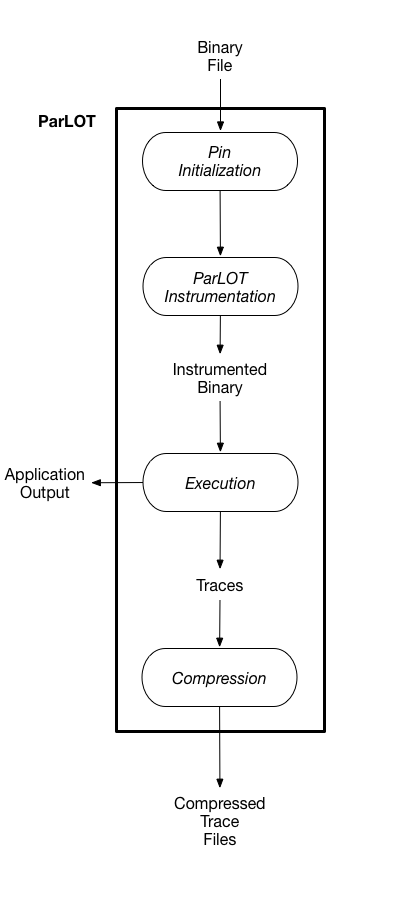
\includegraphics[width=2in]{overview.png}
\caption{Overview of \parlot}
\label{overview}
\end{figure}


\subsection{Evaluation of our Compression Scheme}

We conducted a preliminary evaluation of our compression
scheme by implementing a tracer in PIN that
records a unique 16-bit identifier for every function call and
return. 
%
Tracing just this small amount of information when running the
Mantevo miniapps~\cite{mantevo} on Stampede results in about 2 MB/s of
data per core on average. Extrapolating this value to all 102,400
cores of Stampede (not counting accelerators) yields 205 GB/s of trace
data, which exceeds the Lustre filesystem's write performance of 150
GB/s! 
%
Adding a simple compression algorithm that CRUSHER created 
reduces the emitted trace data by a factor of 100 on average,
a ratio that is very stable w.r.t scaling, making it possible to trace
full-scale programs while leaving over 98\% of the I/O bandwidth to
the application. 
%
This level of compression efficiency is also apparent in the 
results that we will present beginning \S\ref{sec:results}.

%--end



\section{Evaluation Methodology}
\label{sec:evalmeth}
\subsection{Benchmarks and System}

We performed our evaluations on the MPI-based NAS Parallel Benchmarks (NPB)~\cite{nas}.
%
NPB includes four inputs sizes.
%
To keep the runtimes reasonable, we show results for the class \textit{B} (small-medium) and class \textit{C} (medium-large) inputs.
%

We compiled the NPB codes with the mpicc and mpif77 wrappers of MVAPICH 2.2.1, which are based on icc/ifort 14.0.2 using the prescribed -g and -O1 optimization flags.
%
Quick tests showed that higher optimization levels do not significantly improve the performance.
%

We ran all experiments on Comet at the San Diego Supercomputer Center~\cite{comet}, whose filesystem is NSF and Lustre.
%
Comet has 1944 compute nodes, each of which has dual-socket Intel Xeon E5-2680 v3 processors with a total of 28 cores (14 per socket) and 128 GB of main memory.
%
Note that we only used 16 cores per node as many of the NPB programs require a core count that is a power of two.
%
To study the scaling behavior, we ran experiments on 1, 4, 16 and 64 compute nodes, i.e., on up to 1024 cores.


\subsection{Metrics}

We use the following metrics to quantify and compare the performance of the tracing tools.
%
Unless otherwise noted, all results are based on the median of three identical experiments.
%
\begin{itemize}
\item The \textbf{tracing overhead} is the runtime of the target application when it is being traced divided by the runtime of the same application without tracing.
%
This lower-is-better ratio measures by how much the tracing (and the compression when enabled) slows down the target application.
%
\item The \textbf{tracing bandwidth} is the size of the trace information divided by the application runtime.
%
To make the results easier to compare, we generally list the tracing bandwidth per core, i.e., the tracing bandwidth divided by the number of cores used.
%
This lower-is-better metric is expressed in kilobytes per second (kB/s) per core.
%
It specifies the average needed bandwidth to record the trace data.
%
\item The \textbf{compression ratio} is the size of the uncompressed trace divided by the size of the generated (compressed) trace.
%
This higher-is-better ratio measures the factor by which the compression reduces the trace size.
%
In other words, without compression, the tracing bandwidth would be higher by this factor.
\end{itemize}


\subsection{Tracing Tools}
\label{sec:tracing-tools}

We compare our \parlot tool, implemented on top of \pin 3.5, with \callgrind 3.13.
%
\parlot was compiled with gcc 4.9.2 using \pin 's make system and \callgrind with Valgrind's make system.
%
We created the following versions of \parlot to evaluate different aspects of its design.

\begin{itemize}
\item \textbf{\parlotm} is the normal \parlot tool configured to only collect function-call traces from the main image of the application.
\item \textbf{\parlota} is the normal \parlot tool configured to collect function-call traces from all images of the application, including library function calls.
\item \textbf{\pininit} is a crippled version of \parlot from which the tracing code has been removed.
%
The purpose of \pininit is to see how much of the overhead is due to \pin.
\item \textbf{\parlotnc} is the normal \parlot tool but with compression disabled.
%
It writes out the captured data in uncompressed form.
%
The purpose of \parlotnc is to show the performance impact of the compression.
\end{itemize}

It proved surprisingly difficult to find a tool that is similar to \parlot because there appear to be no other tools that generate l{whole program call trace.
%
In the end, we settled on \callgrind as the most similar tool we could find and used it for our comparisons.
%
\callgrind is based on the Valgrind DBI tool.
%
It collects function-call graphs combined with performance data to show the user what portion of the execution time has been spent in each function.

Each \callgrind trace file contains a sequence of function names (or their code) plus numerical data for each function on its caller-callee relationship with other functions.
%
Moreover, it contains cost information for each function in terms of how many machine instructions it read.
%
This information is collected using hardware performance counters.
%
The format of the file is plain ASCII text.
%
Interestingly, all numerical values are expressed relative to previous values, i.e., they are delta (or difference) encoded.
%
This simple form of compression is enabled by default in \callgrind.

%
We believe the information traced by \callgrind is reasonably similar to the information traced by \parlotm.
%
Whereas \callgrind 's traces include performance data that \parlot does not capture, \parlot records the whole-program call trace, which \callgrind does not capture.
%
The full function-call trace is a strict superset of the call-graph information that \callgrind records because the call graph can be extracted from the function-call trace but not vice versa.
%
In particular, \callgrind cannot recreate the order of the function calls a thread made whereas \parlot can.



\section{Results}
\label{sec:results}
%%%%%%%%%%%%%%%%%%%%%%%%%%%%%%%%%%%%%%
% Slowdown vs Callgrind
%%%%%%%%%%%%%%%%%%%%%%%%%%%%%%%%%%%%%




% Original Table

\iffalse

\begin{table*}[]

\caption{Server: \textbf{comet} - 
 Stat: \textbf{sd} - 
 Tools: pinMain , pinAll , callgrind ,  
 Inputs: B , C ,  
 Nodes: 1 , 4 , 16 , 64 ,  
 Desc: Primary --- This table contains Slowdowns of ParLOT and Callgrind (slowdowns are relative to pure run). The input size is \textbf{B}.  NAS benchmark input sizes are as follows : $size(A) < size(B) < size (C) < size(D) $. I grouped the results of experiments with similar input sizes and nodes (group of 3 rows). Each row is in this format \textbf{Tool.Input.Nodes}. Last column of the table (GM) is GeoMean of all values in that row. By comparing the values of GM row, we can see that ParLOT(both main and all) has better performance comparing to Callgrind. However, it seems that Callgrind scales better}
 
\label{comet_sd_pMpAcg_BC_int_p3.5}\begin{center}
\begin{tabular}{|l|rrrrrrrr|r|}
\hline
                &   bt &   cg &    ep &    ft &   is &   lu &   mg &   sp &   GM \\
\hline
 pinMain.B.1    & 1.55 & 1.82 &  2.68 &  2.11 & 2.48 & 1.31 & 2.57 & 1.33 & 1.91 \\
 pinAll.B.1     & 1.85 & 2.73 &  4.21 &  2.85 & 4.52 & 1.74 & 5.57 & 1.73 & 2.87 \\
 callgrind.B.1  & 8.68 & 6.07 &  9.31 & 10.33 & 2.64 & 7.61 & 3.39 & 6.62 & 6.24 \\
\hline
 pinMain.B.4    & 1.76 & 1.85 &  1.92 &  1.74 & 1.79 & 1.77 & 1.83 & 1.76 & 1.80 \\
 pinAll.B.4     & 2.63 & 3.11 &  3.41 &  2.86 & 3.03 & 2.82 & 3.10 & 2.76 & 2.96 \\
 callgrind.B.4  & 6.13 & 3.63 &  2.95 &  3.50 & 1.46 & 5.41 & 1.43 & 5.98 & 3.34 \\
\hline
 pinMain.B.16   & 2.19 & 2.62 &  2.39 &  1.93 & 1.82 & 2.80 & 2.43 & 2.23 & 2.28 \\
 pinAll.B.16    & 3.73 & 4.20 &  4.36 &  2.96 & 2.84 & 4.30 & 4.49 & 3.71 & 3.77 \\
 callgrind.B.16 & 4.31 & 3.26 &  2.39 &  2.20 & 1.73 & 4.70 & 1.92 & 4.65 & 2.93 \\
\hline
 pinMain.B.64   & 2.45 & 2.72 &  2.45 &  1.99 & 4.34 & 4.56 & 2.31 & 2.46 & 2.79 \\
 pinAll.B.64    & 4.22 & 4.19 &  4.55 &  3.13 & 5.46 & 4.73 & 4.17 & 4.23 & 4.29 \\
 callgrind.B.64 & 2.85 & 2.71 &  1.86 &  2.16 & 4.13 & 4.10 & 1.87 & 3.54 & 2.77 \\
\hline
 pinMain.C.1    & 1.41 & 1.29 &  2.51 &  1.90 & 2.34 & 1.12 & 1.76 & 1.11 & 1.61 \\
 pinAll.C.1     & 1.47 & 1.55 &  3.25 &  2.00 & 3.06 & 1.26 & 2.52 & 1.20 & 1.90 \\
 callgrind.C.1  & 8.52 & 4.51 & 13.47 & 13.13 & 3.81 & 7.93 & 6.31 & 5.15 & 7.13 \\
\hline
 pinMain.C.4    & 1.58 & 1.77 &  2.13 &  1.65 & 1.70 & 1.33 & 1.83 & 1.35 & 1.65 \\
 pinAll.C.4     & 1.93 & 2.52 &  3.35 &  2.24 & 2.65 & 1.77 & 3.09 & 1.71 & 2.34 \\
 callgrind.C.4  & 8.83 & 4.55 &  6.52 &  7.04 & 1.74 & 6.83 & 2.89 & 6.48 & 5.03 \\
\hline
 pinMain.C.16   & 1.82 & 2.39 &  2.47 &  1.52 & 1.83 & 2.22 & 2.40 & 1.82 & 2.03 \\
 pinAll.C.16    & 2.70 & 3.47 &  4.27 &  2.15 & 2.80 & 3.21 & 4.30 & 2.75 & 3.13 \\
 callgrind.C.16 & 6.87 & 4.00 &  3.55 &  2.87 & 1.87 & 6.61 & 2.31 & 6.56 & 3.89 \\
\hline
 pinMain.C.64   & 2.32 & 2.74 &  2.48 &  1.61 & 4.49 & 3.52 & 2.68 & 2.28 & 2.65 \\
 pinAll.C.64    & 3.67 & 4.13 &  4.31 &  2.26 & 5.72 & 4.43 & 4.30 & 3.69 & 3.95 \\
 callgrind.C.64 & 4.37 & 3.49 &  2.20 &  2.52 & 4.25 & 5.52 & 2.13 & 4.70 & 3.45 \\
\hline
\end{tabular}
\end{center}
\end{table*}

\fi



%New Table

\iftrue

\begin{table*}[]

\caption{Server: \textbf{comet} - 
 Stat: \textbf{sd} - 
 Tools: pinMain , pinAll , callgrind ,  
 Inputs: B , C ,  
 Nodes: 1 , 4 , 16 , 64 ,  
 Desc: Primary --- This table contains Slowdowns of ParLOT and Callgrind (slowdowns are relative to pure run). The input size is \textbf{B}.  NAS benchmark input sizes are as follows : $size(A) < size(B) < size (C) < size(D) $. I grouped the results of experiments with similar input sizes and nodes (group of 3 rows). Each row is in this format \textbf{Tool.Input.Nodes}. Last column of the table (GM) is GeoMean of all values in that row. By comparing the values of GM row, we can see that ParLOT(both main and all) has better performance comparing to Callgrind. However, it seems that Callgrind scales better}
 
\label{comet_sd_pMpAcg_BC_int_p3.5}
\begin{center}
\begin{tabular}{|c|c|l|rrrrrrrr|r|}
\hline
\multicolumn{1}{|l|}{Input} & \multicolumn{1}{l|}{\# Nodes} & Tool / App & \multicolumn{1}{c}{bt} & \multicolumn{1}{c}{cg} & \multicolumn{1}{c}{ep} & \multicolumn{1}{c}{ft} & \multicolumn{1}{c}{is} & \multicolumn{1}{c}{lu} & \multicolumn{1}{c}{mg} & \multicolumn{1}{c|}{sp} & \multicolumn{1}{c|}{GM} \\ \hline
\multirow{12}{*}{B} & \multirow{3}{*}{1} & ParLOT(main) & 1.55 & 1.82 & 2.68 & 2.11 & 2.48 & 1.31 & 2.57 & 1.33 & 1.91 \\
 &  & ParLOT(all) & 1.85 & 2.73 & 4.21 & 2.85 & 4.52 & 1.74 & 5.57 & 1.73 & 2.87 \\
 &  & Callgrind & 8.68 & 6.07 & 9.31 & 10.33 & 2.64 & 7.61 & 3.39 & 6.62 & 6.24 \\ \cline{2-12} 
 & \multirow{3}{*}{4} & ParLOT(main) & 1.76 & 1.85 & 1.92 & 1.74 & 1.79 & 1.77 & 1.83 & 1.76 & 1.80 \\
 &  & ParLOT(all) & 2.63 & 3.11 & 3.41 & 2.86 & 3.03 & 2.82 & 3.10 & 2.76 & 2.96 \\
 &  & Callgrind & 6.13 & 3.63 & 2.95 & 3.50 & 1.46 & 5.41 & 1.43 & 5.98 & 3.34 \\ \cline{2-12} 
 & \multirow{3}{*}{16} & ParLOT(main) & 2.19 & 2.62 & 2.39 & 1.93 & 1.82 & 2.80 & 2.43 & 2.23 & 2.28 \\
 &  & ParLOT(all) & 3.73 & 4.20 & 4.36 & 2.96 & 2.84 & 4.30 & 4.49 & 3.71 & 3.77 \\
 &  & Callgrind & 4.31 & 3.26 & 2.39 & 2.20 & 1.73 & 4.70 & 1.92 & 4.65 & 2.93 \\ \cline{2-12} 
 & \multirow{3}{*}{64} & ParLOT(main) & 2.45 & 2.72 & 2.45 & 1.99 & 4.34 & 4.56 & 2.31 & 2.46 & 2.79 \\
 &  & ParLOT(all) & 4.22 & 4.19 & 4.55 & 3.13 & 5.46 & 4.73 & 4.17 & 4.23 & 4.29 \\
 &  & Callgrind & 2.85 & 2.71 & 1.86 & 2.16 & 4.13 & 4.10 & 1.87 & 3.54 & 2.77 \\ \hline
\multirow{12}{*}{C} & \multirow{3}{*}{1} & ParLOT(main) & 1.41 & 1.29 & 2.51 & 1.90 & 2.34 & 1.12 & 1.76 & 1.11 & 1.61 \\
 &  & ParLOT(all) & 1.47 & 1.55 & 3.25 & 2.00 & 3.06 & 1.26 & 2.52 & 1.20 & 1.90 \\
 &  & Callgrind & 8.52 & 4.51 & 13.47 & 13.13 & 3.81 & 7.93 & 6.31 & 5.15 & 7.13 \\ \cline{2-12} 
 & \multirow{3}{*}{4} & ParLOT(main) & 1.58 & 1.77 & 2.13 & 1.65 & 1.70 & 1.33 & 1.83 & 1.35 & 1.65 \\
 &  & ParLOT(all) & 1.93 & 2.52 & 3.35 & 2.24 & 2.65 & 1.77 & 3.09 & 1.71 & 2.34 \\
 &  & Callgrind & 8.83 & 4.55 & 6.52 & 7.04 & 1.74 & 6.83 & 2.89 & 6.48 & 5.03 \\ \cline{2-12} 
 & \multirow{3}{*}{16} & ParLOT(main) & 1.82 & 2.39 & 2.47 & 1.52 & 1.83 & 2.22 & 2.40 & 1.82 & 2.03 \\
 &  & ParLOT(all) & 2.70 & 3.47 & 4.27 & 2.15 & 2.80 & 3.21 & 4.30 & 2.75 & 3.13 \\
 &  & Callgrind & 6.87 & 4.00 & 3.55 & 2.87 & 1.87 & 6.61 & 2.31 & 6.56 & 3.89 \\ \cline{2-12} 
 & \multirow{3}{*}{64} & ParLOT(main) & 2.32 & 2.74 & 2.48 & 1.61 & 4.49 & 3.52 & 2.68 & 2.28 & 2.65 \\
 &  & ParLOT(all) & 3.67 & 4.13 & 4.31 & 2.26 & 5.72 & 4.43 & 4.30 & 3.69 & 3.95 \\
 &  & Callgrind & 4.37 & 3.49 & 2.20 & 2.52 & 4.25 & 5.52 & 2.13 & 4.70 & 3.45 \\ \hline
\end{tabular}
\end{center}
\end{table*}

\fi


\begin{table*}[]
\caption{Server: \textbf{comet} - 
 Stat: \textbf{sd} - 
 Tools: pinMain , pinAll , callgrind ,  
 Inputs: B , C ,  
 Nodes: 1 , 4 , 16 , 64 ,  
 Desc: Primary}
\label{comet_sd_pMpAcg_BC_itn_p3.5}\begin{center}
\begin{tabular}{|l|rrrrrrrr|r|}
\hline
                &   bt &   cg &    ep &    ft &   is &   lu &   mg &   sp &   GM \\
\hline
 pinMain.B.1    & 1.55 & 1.82 &  2.68 &  2.11 & 2.48 & 1.31 & 2.57 & 1.33 & 1.91 \\
 pinMain.B.4    & 1.76 & 1.85 &  1.92 &  1.74 & 1.79 & 1.77 & 1.83 & 1.76 & 1.80 \\
 pinMain.B.16   & 2.19 & 2.62 &  2.39 &  1.93 & 1.82 & 2.80 & 2.43 & 2.23 & 2.28 \\
 pinMain.B.64   & 2.45 & 2.72 &  2.45 &  1.99 & 4.34 & 4.56 & 2.31 & 2.46 & 2.79 \\
 \hline
 AVG            & 1.99 & 2.25 &  2.36 &  1.94 & 2.61 & 2.61 & 2.29 & 1.95 & \textbf{2.20} \\
 \hline
 pinAll.B.1     & 1.85 & 2.73 &  4.21 &  2.85 & 4.52 & 1.74 & 5.57 & 1.73 & 2.87 \\
 pinAll.B.4     & 2.63 & 3.11 &  3.41 &  2.86 & 3.03 & 2.82 & 3.10 & 2.76 & 2.96 \\
 pinAll.B.16    & 3.73 & 4.20 &  4.36 &  2.96 & 2.84 & 4.30 & 4.49 & 3.71 & 3.77 \\
 pinAll.B.64    & 4.22 & 4.19 &  4.55 &  3.13 & 5.46 & 4.73 & 4.17 & 4.23 & 4.29 \\
 \hline
 AVG            & 3.11 & 3.56 &  4.13 &  2.95 & 3.96 & 3.40 & 4.33 & 3.11 & \textbf{3.47} \\
 \hline
 callgrind.B.1  & 8.68 & 6.07 &  9.31 & 10.33 & 2.64 & 7.61 & 3.39 & 6.62 & 6.24 \\
 callgrind.B.4  & 6.13 & 3.63 &  2.95 &  3.50 & 1.46 & 5.41 & 1.43 & 5.98 & 3.34 \\
 callgrind.B.16 & 4.31 & 3.26 &  2.39 &  2.20 & 1.73 & 4.70 & 1.92 & 4.65 & 2.93 \\
 callgrind.B.64 & 2.85 & 2.71 &  1.86 &  2.16 & 4.13 & 4.10 & 1.87 & 3.54 & 2.77 \\
 \hline
 AVG            & 5.49 & 3.92 &  4.13 &  4.55 & 2.49 & 5.46 & 2.15 & 5.20 & \textbf{3.82} \\
 \hline
  \hline
 pinMain.C.1    & 1.41 & 1.29 &  2.51 &  1.90 & 2.34 & 1.12 & 1.76 & 1.11 & 1.61 \\
 pinMain.C.4    & 1.58 & 1.77 &  2.13 &  1.65 & 1.70 & 1.33 & 1.83 & 1.35 & 1.65 \\
 pinMain.C.16   & 1.82 & 2.39 &  2.47 &  1.52 & 1.83 & 2.22 & 2.40 & 1.82 & 2.03 \\
 pinMain.C.64   & 2.32 & 2.74 &  2.48 &  1.61 & 4.49 & 3.52 & 2.68 & 2.28 & 2.65 \\
 \hline
 AVG            & 1.78 & 2.05 &  2.40 &  1.67 & 2.59 & 2.05 & 2.17 & 1.64 & \textbf{1.98} \\
 \hline
 pinAll.C.1     & 1.47 & 1.55 &  3.25 &  2.00 & 3.06 & 1.26 & 2.52 & 1.20 & 1.90 \\
 pinAll.C.4     & 1.93 & 2.52 &  3.35 &  2.24 & 2.65 & 1.77 & 3.09 & 1.71 & 2.34 \\
 pinAll.C.16    & 2.70 & 3.47 &  4.27 &  2.15 & 2.80 & 3.21 & 4.30 & 2.75 & 3.13 \\
 pinAll.C.64    & 3.67 & 4.13 &  4.31 &  2.26 & 5.72 & 4.43 & 4.30 & 3.69 & 3.95 \\
 \hline
 AVG            & 2.44 & 2.92 &  3.79 &  2.16 & 3.56 & 2.67 & 3.55 & 2.34 & \textbf{2.83} \\
 \hline
 callgrind.C.1  & 8.52 & 4.51 & 13.47 & 13.13 & 3.81 & 7.93 & 6.31 & 5.15 & 7.13 \\
 callgrind.C.4  & 8.83 & 4.55 &  6.52 &  7.04 & 1.74 & 6.83 & 2.89 & 6.48 & 5.03 \\
 callgrind.C.16 & 6.87 & 4.00 &  3.55 &  2.87 & 1.87 & 6.61 & 2.31 & 6.56 & 3.89 \\
 callgrind.C.64 & 4.37 & 3.49 &  2.20 &  2.52 & 4.25 & 5.52 & 2.13 & 4.70 & 3.45 \\
 \hline
 AVG            & 7.15 & 4.14 &  6.44 &  6.39 & 2.92 & 6.72 & 3.41 & 5.72 & \textbf{4.88} \\
\hline
\end{tabular}
\end{center}
\end{table*}


\subsection{ParLOT vs. Callgrind}

\begin{itemize}
\item \textbf{Slowdown}: Table \ref{comet_sd_pMpAcg_BC_int_p3.5} shows the slowdown of \parlot (pinMain and pinAll) and \callgrind. It shows slowdowns of same configuration (number of nodes/cores and size of input) next to each other so that we can look into it in more detail.
Table \ref{comet_sd_pMpAcg_BC_itn_p3.5} contains same exact numbers but grouped differently. In big picture, as average, by looking at bold numbers of table \ref{comet_sd_pMpAcg_BC_itn_p3.5}, experiments well shows that \parlot has better performance on larger input sizes which means longer runs. But for \callgrind it is opposite. For input size B, the average of geomeans of slowdowns is 3.82 and for input C it is 4.88. The key reason of this better performance is more repetition of target data to collect (which is function calls) on larger input sizes, I believe. Even when \parlot gathers system library function calls (pinAll), it has better performance than \callgrind. Figures \ref{comet_chartAvg_sd_B_p3_5} and \ref{comet_chartAvg_sd_C_p3_5} visualizes table \ref{comet_sd_pMpAcg_BC_itn_p3.5} numbers.
\item \textbf{Bandwidth}: Table \ref{comet_bw_pMpAcg_BC_itn_p3.5} shows the required bandwidth for each tool. In addition to big gap between average slowdown of \parlot(main) and \callgrind, \parlot(main) also beats \callgrind in required bandwidth, especially for smaller inputs.(adapted from Related Tools section) Valgrind is shadow value DBI framework (explained in the background section) that maps and records every register and memory value. It gives developers the capability of instrumenting system calls and instructions. Many error detectors such as \textit{Memcheck} have been built on top of Valgrind. \callgrind is a profiling tool  on Valgrind platform that records the call history among functions in a program's run as a call-graph by measuring the number of instructions executed and their relationship to source lines. 
Intermediate generated traces by \callgrind are some numbered files contain pure ascii text. \callgrind enumerate the name of files and function calls and also, stores those numerical values as relative to previous numbers. These are the only data compression options available on \callgrind which is enabled by default. Each \callgrind trace file contains a sequence of function names (or their code) and a few other numbers for each function showing the that function relationships with other functions (caller-callee). There is a tool \textit{callgrind\_ annotate} which displays different reports from the generated traces. From the generated traces by \callgrind in my experiments, the richest report that \textit{callgrind\_ annotate} can produce is the tree of function calls with caller-callee relationship and cost of each function. Cost of each function is the number of Instruction Read which is collected during tracing by reading hardware counters. Cache simulation and branch prediction information also can be enabled to be collected and then \textit{callgrind\_ annotate} can produce different reports for cache and branch prediction. By default, cache simulation and branch prediction (which are originally from another tool Cachegrind) are disabled by \callgrind.
According to table \ref{comet_cr_pMpA_BC_itn_p3.5}, for example for \parlot(all) where the average compression ratio for input C is 644.38, and the correspondent required bandwidth which is 56.38, it shows that \parlot can collect almost 36 MB worth of data per core per second where it only needs 56.38 KB/S bandwidth.]
\end{itemize}

\begin{figure}[!t]
\centering
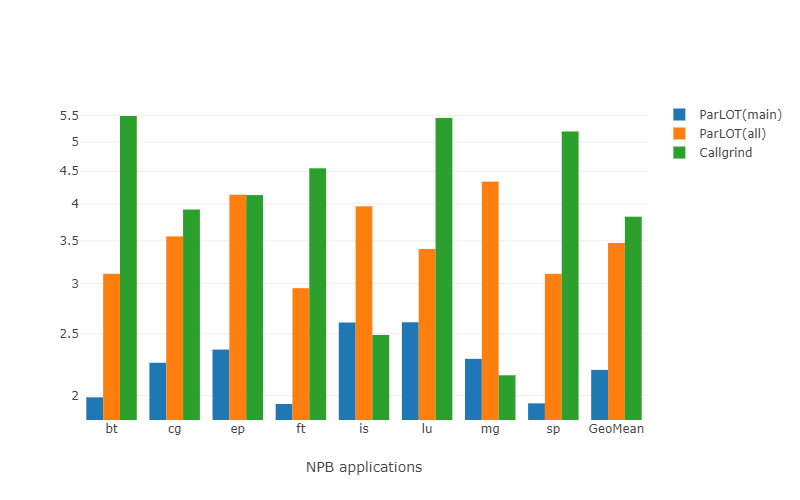
\includegraphics[width=3.9in]{figs.comet/comet_chartAvg_sd_B_p3_5.png}
\caption{ Input: \textbf{B} - Slowdown of \parlot(main,all) and \callgrind. Each bar is the average slowdown of each tool on each application for 1, 4 and 16 nodes (16, 64 and 256 cores). Last group of bars is GeoMean (from bold numbers in table \ref{comet_sd_pMpAcg_BC_itn_p3.5}). 
}
\label{comet_chartAvg_sd_B_p3_5}
\end{figure}


\begin{figure}[!t]
\centering
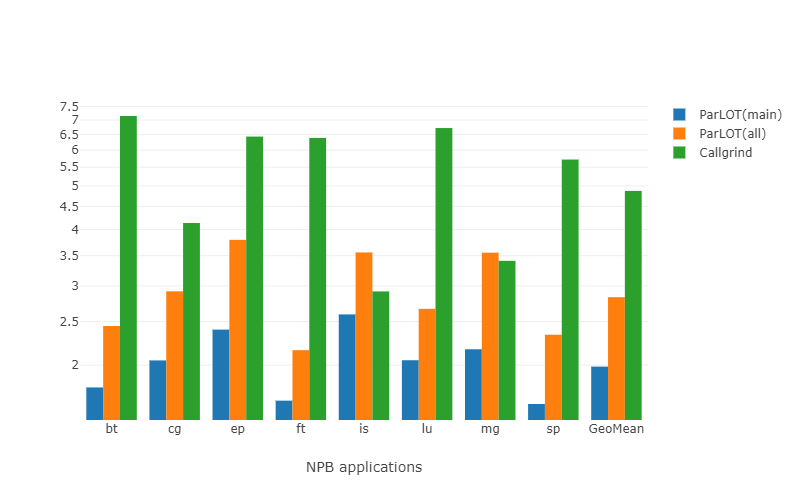
\includegraphics[width=3.9in]{figs.comet/comet_chartAvg_sd_C_p3_5.png}
\caption{ Input: \textbf{C} - Slowdown of \parlot(main,all) and \callgrind. Each bar is the average slowdown of each tool on each application for 1, 4 and 16 nodes (16, 64 and 256 cores). Last group of bars is GeoMean (from bold numbers in table \ref{comet_sd_pMpAcg_BC_itn_p3.5}). 
}
\label{comet_chartAvg_sd_C_p3_5}
\end{figure}




\subsection{\parlot Inner Analysis}
	\begin{itemize}
	\item \textbf{Compression Ratio}: Table \ref{comet_cr_pMpA_BC_itn_p3.5} shows the compression ratios for all configs and inputs. On average, \parlot can store up to more than 1700 MB of collected data in just 1 MB trace files. Compression ratios are higher for larger input sizes (reason: repetition of function calls). Also \parlot has better compression performance when it only collects function calls from main application image.
	\item \textbf{Pure \pin Overhead}: Tables \ref{comet_wo_det_Main_all_B_p3.5}, \ref{comet_wo_det_All_all_B_p3.5}, \ref{comet_wo_det_Main_all_C_p3.5} and  \ref{comet_wo_det_All_all_C_p3.5} show average overhead added to each application by different variations of \parlot. Reason of these experiments is to show the \textbf{impact of our data compression approach} and \textbf{pure overhead added by \pin}. \textbf{npin} is just the slowdown caused by initializing \pin's routines on top of the target application without doing anything else (no instrumentation, tracing, compression). In \textbf{wpin}, all collected data would be stored as is to the disk (tracing without compression) (fig \ref{overviewAll}). Last row of tables shows geometric mean of each of its above values showing how much each phase of ParLOT slows down the native execution. In general, we all expect that the slowdowns of $npin < ParLOT < wpin $. But majority of numbers are not like that. Highlighted cells in tables are the ones which do not follow the above order. Number of highlighted cells for \parlot(main) is larger than \parlot(all). Figures \ref{comet_chartAvg_serr_B_p3_5}, \ref{comet_chartAvg_serr_C_p3_5}, \ref{comet_chartAvg_var_B_p3_5} and  \ref{comet_chartAvg_var_C_p3_5} which are the standard errors and variances of runtimes, explain the reason of these highlighted cells. Variability of runtimes for \parlot(main) is more than other ones (native run, \parlot(all) and \callgrind). Maybe if I put the maximum or average of runtimes in the tables, the number of highlighted cells decreases.\\
	Figures \ref{comet_chartDet_B_wc_byTool_p3_5}, \ref{comet_chartDet_C_wc_byTool_p3_5}, \ref{comet_chartDet_B_woc_byTool_p3_5} and \ref{comet_chartDet_C_woc_byTool_p3_5} clearly show the performance of \parlot and impact of \parlot 's compression mechanism. (more explanations in chart caption of figure \ref{comet_chartDet_B_wc_byTool_p3_5} and \ref{comet_chartDet_B_woc_byTool_p3_5})
	\item \textbf{Impact of Compression} - Figures \ref{comet_chartDet_B_wc_byTool_p3_5}, \ref{comet_chartDet_C_wc_byTool_p3_5}, \ref{comet_chartDet_B_woc_byTool_p3_5} and \ref{comet_chartDet_C_woc_byTool_p3_5}
	\item \textbf{Variability} - Figures \ref{comet_chartAvg_serr_B_p3_5}, \ref{comet_chartAvg_serr_C_p3_5}, \ref{comet_chartAvg_var_B_p3_5} and  \ref{comet_chartAvg_var_C_p3_5}.
	\end{itemize}


\begin{figure}[!t]
\centering
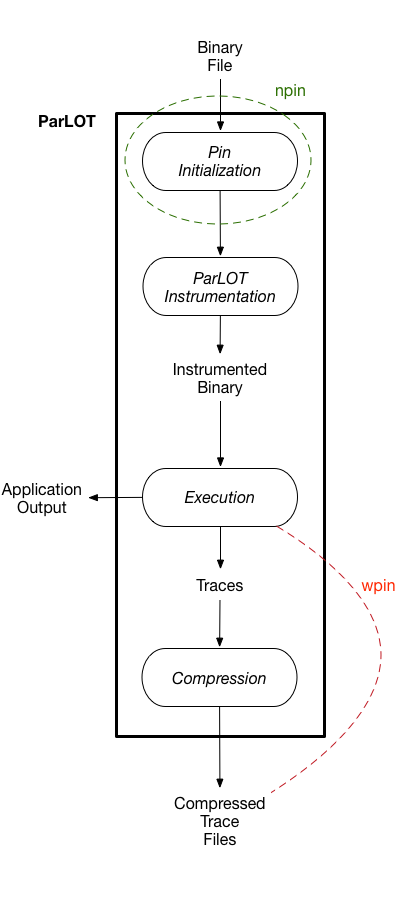
\includegraphics[width=2in]{overview-all.png}
\caption{ Overview of \parlot}
\label{overviewAll}
\end{figure}

%%%%%%%%%%%%%%%%%%%%%%%%%%%%%%%%%%%%%
% Bandwidth
%%%%%%%%%%%%%%%%%%%%%%%%%%%%%%%%%%%%%

%%%%%%%%%%%%%%%%%%%%%%%
% Compression Ratio
%%%%%%%%%%%%%%%%%%%%%%%



\begin{table*}[]
\caption{Server: \textbf{comet} - 
 Stat: \textbf{bw} - 
 Tools: pinMain , pinAll , callgrind ,  
 Inputs: B , C ,  
 Nodes: 1 , 4 , 16 , 64 ,  
 Desc: Primary
This table is showing the required bandwidth for each application (KiloBytes per core per second). $ReqBW_x = TraceSize_x (KB) / (\# of cores)_x / Runtime_x (S)$
. Clearly ParLOT(main) is beating Callgrind while they both generate the same information. ParLOT(all) bandwidth is the highest but with capturing all of the function calls within a single execution, there is no surprise. Figures \ref{comet_chartAvg_bw_B_p3_5} and \ref{comet_chartAvg_bw_C_p3_5} visualize these numbers (Average values) 
 }
\label{comet_bw_pMpAcg_BC_itn_p3.5}\begin{center}
\begin{tabular}{|l|rrrrrrrr|r|}
\hline
                &    bt &     cg &    ep &    ft &    is &     lu &    mg &     sp &    GM \\
\hline
 pinMain.B.1    &  4.72 &  21.86 &  3.83 &  1.52 &  0.79 &   2.39 &  5.62 &   5.36 &  3.69 \\
 pinMain.B.4    & 14.28 &  41.08 &  1.89 &  3.48 &  2.24 &  21.48 &  6.45 &  15.85 &  8.12 \\
 pinMain.B.16   & 14.31 &  46.59 &  1.45 &  4.86 &  3.40 &  31.79 &  6.53 &  18.55 &  9.41 \\
 pinMain.B.64   & 18.56 &  43.59 &  1.25 &  4.56 &  4.49 &  27.07 &  5.63 &  29.62 &  9.92 \\
 \hline
 AVG            & 12.97 &  38.28 &  2.10 &  3.60 &  2.73 &  20.68 &  6.06 &  17.35 &  \textbf{7.79} \\
 \hline
 pinAll.B.1     & 48.71 &  89.39 & 47.23 & 45.63 & 59.98 &  53.62 & 60.81 &  54.33 & 56.21 \\
 pinAll.B.4     & 61.84 & 101.23 & 45.21 & 55.12 & 53.20 &  71.09 & 54.85 &  73.62 & 62.68 \\
 pinAll.B.16    & 73.95 & 116.87 & 47.37 & 48.88 & 47.79 & 100.91 & 55.80 &  84.61 & 67.97 \\
 pinAll.B.64    & 81.80 & 110.15 & 44.16 & 47.98 & 37.84 & 100.26 & 52.67 &  99.90 & 66.47 \\
 \hline
 AVG            & 66.58 & 104.41 & 45.99 & 49.40 & 49.70 &  81.47 & 56.03 &  78.12 & \textbf{63.33} \\
 \hline
 callgrind.B.1  &  1.57 &   7.69 &  7.39 &  4.56 & 39.49 &   2.61 & 34.41 &   2.71 &  6.67 \\
 callgrind.B.4  &  6.51 &  16.01 & 22.10 & 15.65 & 45.46 &   8.63 & 45.47 &   7.78 & 16.31 \\
 callgrind.B.16 & 17.20 &  24.62 & 37.42 & 23.84 & 29.87 &  16.23 & 51.49 &  15.81 & 24.93 \\
 callgrind.B.64 & 26.82 &  27.65 & 45.93 & 25.14 & 11.04 &  17.75 & 45.27 &  20.20 & 25.02 \\
 \hline
 AVG            & 13.03 &  18.99 & 28.21 & 17.30 & 31.47 &  11.30 & 44.16 &  11.62 & \textbf{18.23} \\
 \hline
 \hline
 pinMain.C.1    &  1.82 &  16.96 &  5.15 &  1.16 &  0.69 &   0.77 &  3.56 &   1.40 &  2.17 \\
 pinMain.C.4    &  7.53 &  44.87 &  3.00 &  2.50 &  2.12 &  20.13 &  7.08 &  13.74 &  7.55 \\
 pinMain.C.16   & 16.30 &  55.04 &  1.84 &  6.10 &  3.35 &  34.09 &  7.24 &  20.68 & 10.70 \\
 pinMain.C.64   & 17.45 &  61.43 &  1.30 &  5.93 &  4.42 &  38.28 &  5.62 &  26.09 & 10.94 \\
 \hline
 AVG            & 10.77 &  44.58 &  2.82 &  3.92 &  2.65 &  23.32 &  5.88 &  15.48 &  \textbf{7.84} \\
 \hline
 pinAll.C.1     & 17.80 &  53.37 & 26.34 & 20.89 & 48.31 &  25.31 & 52.61 &  19.46 & 29.99 \\
 pinAll.C.4     & 51.78 &  95.84 & 36.80 & 43.82 & 51.40 &  58.39 & 54.18 &  65.77 & 55.15 \\
 pinAll.C.16    & 75.38 & 121.03 & 44.29 & 61.39 & 46.90 & 101.05 & 56.49 & 101.32 & 71.37 \\
 pinAll.C.64    & 80.63 & 135.19 & 43.49 & 46.28 & 37.09 & 117.87 & 54.05 &  99.02 & 68.99 \\
 \hline
 AVG            & 56.40 & 101.36 & 37.73 & 43.09 & 45.93 &  75.66 & 54.33 &  71.39 & \textbf{56.38} \\
 \hline
 callgrind.C.1  &  0.40 &   3.09 &  1.96 &  1.05 & 14.60 &   0.70 &  6.96 &   0.75 &  1.85 \\
 callgrind.C.4  &  1.78 &   8.87 &  7.74 &  4.48 & 31.74 &   2.82 & 21.03 &   2.78 &  6.41 \\
 callgrind.C.16 &  6.01 &  15.82 & 22.86 & 10.75 & 26.50 &   7.45 & 39.05 &   6.96 & 13.72 \\
 callgrind.C.64 & 14.32 &  19.56 & 35.75 & 12.17 & 11.07 &  11.86 & 40.69 &  12.83 & 17.39 \\
 \hline
 AVG            &  5.63 &  11.84 & 17.08 &  7.11 & 20.98 &   5.71 & 26.93 &   5.83 &  \textbf{9.84} \\
\hline
\end{tabular}
\end{center}
\end{table*}


\begin{figure}[!t]
\centering
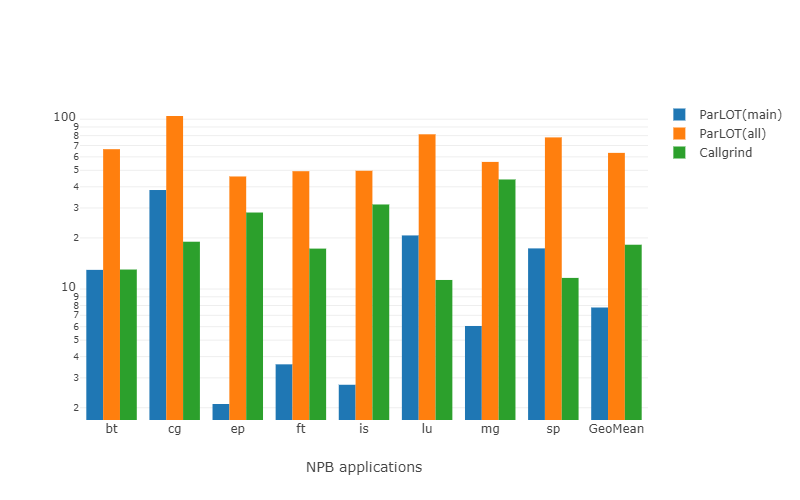
\includegraphics[width=3.5in]{figs.comet/comet_chartAvg_bw_B_p3_5.png}
\caption{ Input: \textbf{B} - Required Bandwidth per core (KB/s)
}
\label{comet_chartAvg_bw_B_p3_5}
\end{figure}

\begin{figure}[!t]
\centering
\includegraphics[width=3.5in]{figs.comet/comet_chartAvg_bw_C_p3_5.png}
\caption{ Input: \textbf{C}  - Required Bandwidth per core (KB/s)
}
\label{comet_chartAvg_bw_C_p3_5}
\end{figure}



%%%%%%%%%%%%%%%%%%%%%%%
% Detail runtimes
%%%%%%%%%%%%%%%%%%%%%%%

\begin{table*}[]
\caption{Server: \textbf{comet} - 
 Stat: \textbf{cr} - 
 Tools: pinMain , pinAll ,  
 Inputs: B , C ,  
 Nodes: 1 , 4 , 16 , 64 ,  
 Desc: Primary}
\label{comet_cr_pMpA_BC_itn_p3.5}\begin{center}
\begin{tabular}{|l|rrrrrrrr|r|}
\hline
              &      bt &     cg &       ep &       ft &       is &     lu &     mg &      sp &      GM \\
\hline
 pinMain.B.1  & 3035.93 &  94.35 & 12456.18 & 12173.49 &  9718.38 & 167.72 &  99.08 &  878.27 & 1255.17 \\
 pinMain.B.4  &  586.64 &  82.48 & 10368.41 &  1737.09 &   909.20 & 140.29 & 254.95 &  338.16 &  559.36 \\
 pinMain.B.16 &  346.66 & 113.28 &  8563.85 &  1077.35 &  1200.57 & 178.98 & 387.63 &  123.02 &  496.83 \\
 pinMain.B.64 &  252.24 & 147.78 &  7611.04 &  1122.62 &  1907.95 & 366.80 & 437.31 &  152.91 &  591.11 \\
 \hline
 AVG          & 1055.37 & 109.47 &  9749.87 &  4027.64 &  3434.03 & 213.45 & 294.74 &  373.09 &  \textbf{725.62} \\
 \hline
 pinAll.B.1   &  514.51 & 137.41 &  3335.77 &  1226.74 &   543.18 & 314.63 & 260.87 &  303.88 &  500.21 \\
 pinAll.B.4   &  315.71 & 137.21 &  1266.92 &   436.15 &   316.16 & 287.25 & 329.57 &  199.66 &  330.70 \\
 pinAll.B.16  &  226.86 & 181.58 &  1246.66 &  1026.53 &   927.09 & 299.30 & 469.29 &  171.52 &  430.39 \\
 pinAll.B.64  &  329.23 & 247.30 &  1394.07 &  1043.94 &  1984.62 & 410.32 & 548.47 &  307.16 &  597.55 \\
 \hline
 AVG          &  346.58 & 175.88 &  1810.86 &   933.34 &   942.76 & 327.88 & 402.05 &  245.56 &  \textbf{464.71} \\
 \hline
 \hline
 pinMain.C.1  & 8618.95 & 111.16 & 13067.96 & 21335.57 & 21856.49 & 350.03 & 247.44 & 1977.43 & 2371.35 \\
 pinMain.C.4  & 1910.64 & 110.45 & 12418.66 &  6520.34 &  2256.56 & 112.77 & 267.98 &  472.68 &  928.16 \\
 pinMain.C.16 &  580.79 & 133.24 & 11017.36 &  1239.31 &  1347.88 & 164.47 & 396.86 &  143.13 &  582.78 \\
 pinMain.C.64 &  322.83 & 131.92 &  9154.99 &  1065.12 &  1896.25 & 223.69 & 465.74 &  168.89 &  585.74 \\
 \hline
 AVG          & 2858.30 & 121.69 & 11414.74 &  7540.09 &  6839.30 & 212.74 & 344.50 &  690.53 & \textbf{1117.01} \\
 \hline
 pinAll.C.1   & 2579.37 & 181.76 &  7376.96 &  5143.08 &  1520.42 & 408.21 & 314.77 &  650.73 & 1107.37 \\
 pinAll.C.4   &  448.61 & 161.32 &  3194.58 &  1062.94 &   527.34 & 274.70 & 319.35 &  237.43 &  477.42 \\
 pinAll.C.16  &  285.05 & 185.74 &  1765.49 &   588.86 &  1106.34 & 273.63 & 467.35 &  141.69 &  426.92 \\
 pinAll.C.64  &  290.00 & 214.68 &  1512.89 &  1237.30 &  2038.72 & 329.04 & 496.21 &  270.83 &  565.82 \\
 \hline
 AVG          &  900.76 & 185.88 &  3462.48 &  2008.05 &  1298.21 & 321.39 & 399.42 &  325.17 &  \textbf{644.38} \\
\hline
\end{tabular}
\end{center}
\end{table*}




\begin{table*}[]
\caption{Server: \textbf{comet} - 
 Stat: \textbf{sd} - 
 Tools:  
 Inputs: B ,  
 Nodes: 1 , 4 , 16 , 64 ,  
 Desc: Detail Report}
\begin{center}
\label{comet_wo_det_Main_all_B_p3.5}
\scalebox{0.95}{
\begin{tabular}{|c|c|rrr|rrr|rrr|rrr|} 
\hline 
\multicolumn{1}{|l|}{\multirow{2}{*}{\textbf{Input: B}}} & \multicolumn{1}{r|}{Nodes :}    & \multicolumn{3}{c|}{1}  & \multicolumn{3}{c|}{4} & \multicolumn{3}{c|}{16}  & \multicolumn{3}{c|}{64} \\ \cline{2-14} 
\multicolumn{1}{|l|}{} & \multicolumn{1}{r|}{Detail Tools:} & \multicolumn{1}{c}{npin} & \multicolumn{1}{c}{ParLOT} & \multicolumn{1}{c|}{wpin} & \multicolumn{1}{c}{npin} & \multicolumn{1}{c}{ParLOT} & \multicolumn{1}{c|}{wpin} & \multicolumn{1}{c}{npin} & \multicolumn{1}{c}{ParLOT} & \multicolumn{1}{c|}{wpin} & \multicolumn{1}{c}{npin} & \multicolumn{1}{c}{ParLOT} & \multicolumn{1}{c|}{wpin} \\
\hline
\multirow{9}{*}{Main} &  bt  &  1.50  &  1.55  &   5.66  &  1.74  &  1.76  &  5.19  &  2.21  & \cellcolor{blue!25} 2.19  &  5.98  &  2.29  &  2.45  &  5.42 \\
 &  cg  &  1.75  &  1.82  &   2.39  &  1.95  & \cellcolor{blue!25} 1.85  &  2.64  &  2.72  & \cellcolor{blue!25} 2.62  &  5.06  &  2.67  &  2.72  &  7.01 \\
 &  ep  &  2.97  & \cellcolor{blue!25} 2.68  &  21.44  &  2.07  & \cellcolor{blue!25} 1.92  &  5.82  &  2.58  & \cellcolor{blue!25} 2.39  &  3.76  &  2.81  & \cellcolor{blue!25} 2.45  &  2.85 \\
 &  ft  &  1.87  &  2.11  &   6.29  &  1.76  & \cellcolor{blue!25} 1.74  &  2.85  &  2.13  & \cellcolor{blue!25} 1.93  &  2.25  &  2.23  & \cellcolor{blue!25} 1.99  &  2.22 \\
 &  is  &  2.51  & \cellcolor{blue!25} 2.48  &   4.87  &  1.80  & \cellcolor{blue!25} 1.79  &  2.08  &  2.11  & \cellcolor{blue!25} 1.82  &  1.90  &  4.76  & \cellcolor{blue!25} 4.34  &  5.75 \\
 &  lu  &  1.32  & \cellcolor{blue!25} 1.31  &   1.44  &  1.77  &  1.77  &  2.27  &  2.74  &  2.80  &  3.63  &  3.05  &  4.56  &  6.64 \\
 &  mg  &  2.64  & \cellcolor{blue!25} 2.57  &   2.80  &  1.75  &  1.83  &  1.79  &  2.64  & \cellcolor{blue!25} 2.43  &  2.73  &  2.37  & \cellcolor{blue!25} 2.31  &  2.49 \\
 &  sp  &  1.35  & \cellcolor{blue!25} 1.33  &   2.47  &  1.74  &  1.76  &  3.72  &  2.15  &  2.23  &  2.52  &  2.29  &  2.46  &  3.65 \\
 &  GM  &  1.90  &  1.91  &   4.15  &  1.82  & \cellcolor{blue!25} 1.80  &  3.03  &  2.40  & \cellcolor{blue!25} 2.28  &  3.24  &  2.72  &  2.79  &  4.12 \\
\hline 
\end{tabular} }

\end{center}
\end{table*}


\begin{table*}[]
\caption{Server: \textbf{comet} - 
 Stat: \textbf{sd} - 
 Tools:  
 Inputs: B ,  
 Nodes: 1 , 4 , 16 , 64 ,  
 Desc: Detail Report}
\begin{center}
\label{comet_wo_det_All_all_B_p3.5}
\scalebox{0.95}{
\begin{tabular}{|c|c|rrr|rrr|rrr|rrr|} 
\hline 
\multicolumn{1}{|l|}{\multirow{2}{*}{\textbf{Input: B}}} & \multicolumn{1}{r|}{Nodes :}    & \multicolumn{3}{c|}{1}  & \multicolumn{3}{c|}{4} & \multicolumn{3}{c|}{16}  & \multicolumn{3}{c|}{64} \\ \cline{2-14} 
\multicolumn{1}{|l|}{} & \multicolumn{1}{r|}{Detail Tools:} & \multicolumn{1}{c}{npin} & \multicolumn{1}{c}{ParLOT} & \multicolumn{1}{c|}{wpin} & \multicolumn{1}{c}{npin} & \multicolumn{1}{c}{ParLOT} & \multicolumn{1}{c|}{wpin} & \multicolumn{1}{c}{npin} & \multicolumn{1}{c}{ParLOT} & \multicolumn{1}{c|}{wpin} & \multicolumn{1}{c}{npin} & \multicolumn{1}{c}{ParLOT} & \multicolumn{1}{c|}{wpin} \\
\hline
\multirow{9}{*}{All} &  bt  &  1.76  &  1.85  &   6.23  &  2.39  &  2.63  &  6.39  &  3.40  &  3.73  &  10.64  &  3.74  &  4.22  &   9.47 \\
 &  cg  &  2.72  &  2.73  &   3.80  &  2.88  &  3.11  &  4.64  &  4.08  &  4.20  &  16.45  &  4.10  &  4.19  &  14.32 \\
 &  ep  &  4.42  & \cellcolor{blue!25} 4.21  &  23.24  &  3.25  &  3.41  &  7.16  &  4.27  &  4.36  &   5.67  &  4.43  &  4.55  &   5.13 \\
 &  ft  &  2.82  &  2.85  &   6.98  &  2.65  &  2.86  &  3.85  &  2.96  &  2.96  &   4.66  &  3.60  & \cellcolor{blue!25} 3.13  &   3.91 \\
 &  is  &  4.67  & \cellcolor{blue!25} 4.52  &   7.14  &  2.89  &  3.03  &  3.45  &  3.02  & \cellcolor{blue!25} 2.84  &   3.46  &  5.43  &  5.46  &  11.41 \\
 &  lu  &  1.71  &  1.74  &   2.41  &  2.54  &  2.82  &  4.91  &  4.09  &  4.30  &  11.60  &  4.48  &  4.73  &  25.53 \\
 &  mg  &  4.93  &  5.57  &   5.66  &  2.80  &  3.10  &  3.17  &  4.35  &  4.49  &   5.34  &  3.98  &  4.17  &   5.31 \\
 &  sp  &  1.70  &  1.73  &   3.13  &  2.54  &  2.76  &  5.32  &  3.43  &  3.71  &   7.39  &  3.66  &  4.23  &  22.13 \\
 &  GM  &  2.82  &  2.87  &   5.74  &  2.73  &  2.96  &  4.69  &  3.66  &  3.77  &   7.21  &  4.14  &  4.29  &   9.91 \\
\hline 
\end{tabular} }

\end{center}
\end{table*}



\begin{table*}[]
\caption{Server: \textbf{comet} - 
 Stat: \textbf{sd} - 
 Tools:  
 Inputs: C ,  
 Nodes: 1 , 4 , 16 , 64 ,  
 Desc: Detail Report}
\begin{center}
\label{comet_wo_det_Main_all_C_p3.5}
\scalebox{0.95}{
\begin{tabular}{|c|c|rrr|rrr|rrr|rrr|} 
\hline 
\multicolumn{1}{|l|}{\multirow{2}{*}{\textbf{Input: C}}} & \multicolumn{1}{r|}{Nodes :}    & \multicolumn{3}{c|}{1}  & \multicolumn{3}{c|}{4} & \multicolumn{3}{c|}{16}  & \multicolumn{3}{c|}{64} \\ \cline{2-14} 
\multicolumn{1}{|l|}{} & \multicolumn{1}{r|}{Detail Tools:} & \multicolumn{1}{c}{npin} & \multicolumn{1}{c}{ParLOT} & \multicolumn{1}{c|}{wpin} & \multicolumn{1}{c}{npin} & \multicolumn{1}{c}{ParLOT} & \multicolumn{1}{c|}{wpin} & \multicolumn{1}{c}{npin} & \multicolumn{1}{c}{ParLOT} & \multicolumn{1}{c|}{wpin} & \multicolumn{1}{c}{npin} & \multicolumn{1}{c}{ParLOT} & \multicolumn{1}{c|}{wpin} \\
\hline
\multirow{9}{*}{Main} &  bt  &  1.36  &  1.41  &   5.36  &  1.53  &  1.58  &   5.86  &  2.09  & \cellcolor{blue!25} 1.82  &   6.05  &  2.10  &  2.32  &   5.76 \\
 &  cg  &  1.27  &  1.29  &   1.75  &  1.68  &  1.77  &   3.02  &  2.82  & \cellcolor{blue!25} 2.39  &   6.19  &  2.83  & \cellcolor{blue!25} 2.74  &  15.57 \\
 &  ep  &  2.95  & \cellcolor{blue!25} 2.51  &  30.50  &  2.27  & \cellcolor{blue!25} 2.13  &  14.23  &  2.83  & \cellcolor{blue!25} 2.47  &  10.32  &  2.58  & \cellcolor{blue!25} 2.48  &   3.84 \\
 &  ft  &  1.50  &  1.90  &   9.21  &  1.56  &  1.65  &   5.23  &  1.70  & \cellcolor{blue!25} 1.52  &   3.27  &  1.75  & \cellcolor{blue!25} 1.61  &   2.23 \\
 &  is  &  2.26  &  2.34  &   7.28  &  1.72  & \cellcolor{blue!25} 1.70  &   2.75  &  2.05  & \cellcolor{blue!25} 1.83  &   2.34  &  4.73  & \cellcolor{blue!25} 4.49  &   6.66 \\
 &  lu  &  1.12  &  1.12  &   1.19  &  1.32  &  1.33  &   1.59  &  2.16  &  2.22  &   3.95  &  2.95  &  3.52  &   9.77 \\
 &  mg  &  1.75  &  1.76  &   2.02  &  1.84  & \cellcolor{blue!25} 1.83  &   2.03  &  2.47  & \cellcolor{blue!25} 2.40  &   2.86  &  2.47  &  2.68  &   3.28 \\
 &  sp  &  1.10  &  1.11  &   1.63  &  1.36  & \cellcolor{blue!25} 1.35  &   2.88  &  1.78  &  1.82  &   2.38  &  2.11  &  2.28  &   5.58 \\
 &  GM  &  1.57  &  1.61  &   4.07  &  1.64  &  1.65  &   3.68  &  2.20  & \cellcolor{blue!25} 2.03  &   4.10  &  2.58  &  2.65  &   5.56 \\
\hline 
\end{tabular} }

\end{center}
\end{table*}


\begin{table*}[]
\caption{Server: \textbf{comet} - 
 Stat: \textbf{sd} - 
 Tools:  
 Inputs: C ,  
 Nodes: 1 , 4 , 16 , 64 ,  
 Desc: Detail Report}
\begin{center}
\label{comet_wo_det_All_all_C_p3.5}
\scalebox{0.95}{
\begin{tabular}{|c|c|rrr|rrr|rrr|rrr|} 
\hline 
\multicolumn{1}{|l|}{\multirow{2}{*}{\textbf{Input: C}}} & \multicolumn{1}{r|}{Nodes :}    & \multicolumn{3}{c|}{1}  & \multicolumn{3}{c|}{4} & \multicolumn{3}{c|}{16}  & \multicolumn{3}{c|}{64} \\ \cline{2-14} 
\multicolumn{1}{|l|}{} & \multicolumn{1}{r|}{Detail Tools:} & \multicolumn{1}{c}{npin} & \multicolumn{1}{c}{ParLOT} & \multicolumn{1}{c|}{wpin} & \multicolumn{1}{c}{npin} & \multicolumn{1}{c}{ParLOT} & \multicolumn{1}{c|}{wpin} & \multicolumn{1}{c}{npin} & \multicolumn{1}{c}{ParLOT} & \multicolumn{1}{c|}{wpin} & \multicolumn{1}{c}{npin} & \multicolumn{1}{c}{ParLOT} & \multicolumn{1}{c|}{wpin} \\
\hline
\multirow{9}{*}{All} &  bt  &  1.43  &  1.47  &   5.31  &  1.79  &  1.93  &   6.32  &  2.51  &  2.70  &   8.84  &  3.20  &  3.67  &   9.67 \\
 &  cg  &  1.57  & \cellcolor{blue!25} 1.55  &   2.08  &  2.44  &  2.52  &   4.35  &  3.74  & \cellcolor{blue!25} 3.47  &  11.74  &  4.13  &  4.13  &  17.15 \\
 &  ep  &  3.56  & \cellcolor{blue!25} 3.25  &  30.05  &  3.16  &  3.35  &  14.92  &  4.15  &  4.27  &   9.10  &  4.25  &  4.31  &   5.40 \\
 &  ft  &  1.78  &  2.00  &   9.55  &  2.15  &  2.24  &   5.60  &  2.09  &  2.15  &   4.40  &  2.29  & \cellcolor{blue!25} 2.26  &   3.35 \\
 &  is  &  3.35  & \cellcolor{blue!25} 3.06  &   8.20  &  2.65  &  2.65  &   3.86  &  2.95  & \cellcolor{blue!25} 2.80  &   3.53  &  5.59  &  5.72  &   8.98 \\
 &  lu  &  1.23  &  1.26  &   1.52  &  1.70  &  1.77  &   2.94  &  3.09  &  3.21  &   8.28  &  4.22  &  4.43  &  19.13 \\
 &  mg  &  2.67  & \cellcolor{blue!25} 2.52  &   2.96  &  2.92  &  3.09  &   3.32  &  4.04  &  4.30  &   4.81  &  4.04  &  4.30  &   5.25 \\
 &  sp  &  1.17  &  1.20  &   1.67  &  1.65  &  1.71  &   3.57  &  2.56  &  2.75  &   5.38  &  3.16  &  3.69  &  10.48 \\
 &  GM  &  1.92  & \cellcolor{blue!25} 1.90  &   4.58  &  2.24  &  2.34  &   4.86  &  3.06  &  3.13  &   6.49  &  3.75  &  3.95  &   8.54 \\
\hline 
\end{tabular} }

\end{center}
\end{table*}





\begin{table*}[]
\caption{Server: \textbf{comet} - 
 Stat: \textbf{sd} - 
 Tools:  
 Inputs: B ,  
 Nodes: 1 , 4 , 16 , 64 ,  
 Desc: Detail Report}
\begin{center}
\label{comet_wa_det_Main_all_B_p3.5}
\scalebox{0.95}{
\begin{tabular}{|c|c|rrrr|rrrr|rrrr|rrrr|} 
\hline 
\multicolumn{1}{|l|}{\multirow{2}{*}{\textbf{Input: B}}} & \multicolumn{1}{r|}{Nodes :}    & \multicolumn{4}{c|}{1}  & \multicolumn{4}{c|}{4} & \multicolumn{4}{c|}{16}  & \multicolumn{4}{c|}{64} \\ \cline{2-18} 
\multicolumn{1}{|l|}{} & \multicolumn{1}{r|}{Detail Tools:} & \multicolumn{1}{c}{npin} & \multicolumn{1}{c}{apin} & \multicolumn{1}{c}{ParLOT} & \multicolumn{1}{c|}{wpin} & \multicolumn{1}{c}{npin} & \multicolumn{1}{c}{apin} & \multicolumn{1}{c}{ParLOT} & \multicolumn{1}{c|}{wpin} & \multicolumn{1}{c}{npin} & \multicolumn{1}{c}{apin} & \multicolumn{1}{c}{ParLOT} & \multicolumn{1}{c|}{wpin} & \multicolumn{1}{c}{npin} & \multicolumn{1}{c}{apin} & \multicolumn{1}{c}{ParLOT} & \multicolumn{1}{c|}{wpin} \\
\hline
\multirow{9}{*}{Main} &  bt  &  1.50  &  1.56  & \cellcolor{blue!25} 1.55  &   5.66  &  1.74  &  1.78  & \cellcolor{blue!25} 1.76  &  5.19  &  2.21  &  2.25  & \cellcolor{blue!25} 2.19  &  5.98  &  2.29  &  2.50  & \cellcolor{blue!25} 2.45  &  5.42 \\
 &  cg  &  1.75  &  1.81  &  1.82  &   2.39  &  1.95  & \cellcolor{blue!25} 1.84  &  1.85  &  2.64  &  2.72  &  2.72  & \cellcolor{blue!25} 2.62  &  5.06  &  2.67  & \cellcolor{blue!25} 2.53  &  2.72  &  7.01 \\
 &  ep  &  2.97  & \cellcolor{blue!25} 2.69  & \cellcolor{blue!25} 2.68  &  21.44  &  2.07  & \cellcolor{blue!25} 1.91  &  1.92  &  5.82  &  2.58  & \cellcolor{blue!25} 2.38  &  2.39  &  3.76  &  2.81  & \cellcolor{blue!25} 2.50  & \cellcolor{blue!25} 2.45  &  2.85 \\
 &  ft  &  1.87  &  2.11  &  2.11  &   6.29  &  1.76  & \cellcolor{blue!25} 1.74  &  1.74  &  2.85  &  2.13  & \cellcolor{blue!25} 1.85  &  1.93  &  2.25  &  2.23  & \cellcolor{blue!25} 1.96  &  1.99  &  2.22 \\
 &  is  &  2.51  & \cellcolor{blue!25} 2.47  &  2.48  &   4.87  &  1.80  &  1.81  & \cellcolor{blue!25} 1.79  &  2.08  &  2.11  & \cellcolor{blue!25} 1.86  & \cellcolor{blue!25} 1.82  &  1.90  &  4.76  & \cellcolor{blue!25} 4.31  &  4.34  &  5.75 \\
 &  lu  &  1.32  & \cellcolor{blue!25} 1.31  &  1.31  &   1.44  &  1.77  & \cellcolor{blue!25} 1.76  &  1.77  &  2.27  &  2.74  & \cellcolor{blue!25} 2.65  &  2.80  &  3.63  &  3.05  & \cellcolor{blue!25} 2.90  &  4.56  &  6.64 \\
 &  mg  &  2.64  & \cellcolor{blue!25} 2.59  & \cellcolor{blue!25} 2.57  &   2.80  &  1.75  & \cellcolor{blue!25} 1.72  &  1.83  &  1.79  &  2.64  & \cellcolor{blue!25} 2.41  &  2.43  &  2.73  &  2.37  &  2.44  & \cellcolor{blue!25} 2.31  &  2.49 \\
 &  sp  &  1.35  & \cellcolor{blue!25} 1.34  & \cellcolor{blue!25} 1.33  &   2.47  &  1.74  &  1.78  & \cellcolor{blue!25} 1.76  &  3.72  &  2.15  & \cellcolor{blue!25} 2.07  &  2.23  &  2.52  &  2.29  &  2.46  &  2.46  &  3.65 \\
 &  GM  &  1.90  &  1.91  &  1.91  &   4.15  &  1.82  & \cellcolor{blue!25} 1.79  &  1.80  &  3.03  &  2.40  & \cellcolor{blue!25} 2.25  &  2.28  &  3.24  &  2.72  & \cellcolor{blue!25} 2.64  &  2.79  &  4.12 \\
\hline 
\end{tabular} }

\end{center}
\end{table*}


\begin{table*}[]
\caption{(Temporary) Server: \textbf{comet} - 
 Stat: \textbf{sd} - 
 Tools:  
 Inputs: B ,  
 Nodes: 1 , 4 , 16 , 64 ,  
 Desc: Detail Report}
\begin{center}
\label{comet_wa_det_All_all_B_p3.5}
\scalebox{0.95}{
\begin{tabular}{|c|c|rrrr|rrrr|rrrr|rrrr|} 
\hline 
\multicolumn{1}{|l|}{\multirow{2}{*}{\textbf{Input: B}}} & \multicolumn{1}{r|}{Nodes :}    & \multicolumn{4}{c|}{1}  & \multicolumn{4}{c|}{4} & \multicolumn{4}{c|}{16}  & \multicolumn{4}{c|}{64} \\ \cline{2-18} 
\multicolumn{1}{|l|}{} & \multicolumn{1}{r|}{Detail Tools:} & \multicolumn{1}{c}{npin} & \multicolumn{1}{c}{apin} & \multicolumn{1}{c}{ParLOT} & \multicolumn{1}{c|}{wpin} & \multicolumn{1}{c}{npin} & \multicolumn{1}{c}{apin} & \multicolumn{1}{c}{ParLOT} & \multicolumn{1}{c|}{wpin} & \multicolumn{1}{c}{npin} & \multicolumn{1}{c}{apin} & \multicolumn{1}{c}{ParLOT} & \multicolumn{1}{c|}{wpin} & \multicolumn{1}{c}{npin} & \multicolumn{1}{c}{apin} & \multicolumn{1}{c}{ParLOT} & \multicolumn{1}{c|}{wpin} \\
\hline
\multirow{9}{*}{All} &  bt  &  1.76  &  1.86  & \cellcolor{blue!25} 1.85  &   6.23  &  2.39  &  2.59  &  2.63  &  6.39  &  3.40  &  3.69  &  3.73  &  10.64  &  3.74  &  3.98  &  4.22  &   9.47 \\
 &  cg  &  2.72  &  2.72  &  2.73  &   3.80  &  2.88  &  2.96  &  3.11  &  4.64  &  4.08  & \cellcolor{blue!25} 4.02  &  4.20  &  16.45  &  4.10  &  4.11  &  4.19  &  14.32 \\
 &  ep  &  4.42  & \cellcolor{blue!25} 4.22  & \cellcolor{blue!25} 4.21  &  23.24  &  3.25  &  3.34  &  3.41  &  7.16  &  4.27  &  4.28  &  4.36  &   5.67  &  4.43  & \cellcolor{blue!25} 4.39  &  4.55  &   5.13 \\
 &  ft  &  2.82  &  2.97  & \cellcolor{blue!25} 2.85  &   6.98  &  2.65  &  2.73  &  2.86  &  3.85  &  2.96  & \cellcolor{blue!25} 2.94  &  2.96  &   4.66  &  3.60  & \cellcolor{blue!25} 3.07  &  3.13  &   3.91 \\
 &  is  &  4.67  & \cellcolor{blue!25} 4.48  &  4.52  &   7.14  &  2.89  &  3.06  & \cellcolor{blue!25} 3.03  &  3.45  &  3.02  & \cellcolor{blue!25} 2.84  &  2.84  &   3.46  &  5.43  & \cellcolor{blue!25} 5.34  &  5.46  &  11.41 \\
 &  lu  &  1.71  &  1.73  &  1.74  &   2.41  &  2.54  &  2.80  &  2.82  &  4.91  &  4.09  &  4.21  &  4.30  &  11.60  &  4.48  & \cellcolor{blue!25} 4.33  &  4.73  &  25.53 \\
 &  mg  &  4.93  &  5.27  &  5.57  &   5.66  &  2.80  &  3.06  &  3.10  &  3.17  &  4.35  &  4.40  &  4.49  &   5.34  &  3.98  &  4.38  & \cellcolor{blue!25} 4.17  &   5.31 \\
 &  sp  &  1.70  &  1.71  &  1.73  &   3.13  &  2.54  &  2.68  &  2.76  &  5.32  &  3.43  &  3.59  &  3.71  &   7.39  &  3.66  &  3.79  &  4.23  &  22.13 \\
 &  GM  &  2.82  &  2.86  &  2.87  &   5.74  &  2.73  &  2.89  &  2.96  &  4.69  &  3.66  &  3.70  &  3.77  &   7.21  &  4.14  & \cellcolor{blue!25} 4.13  &  4.29  &   9.91 \\
\hline 
\end{tabular} }

\end{center}
\end{table*}



\begin{table*}[]
\caption{Server: \textbf{comet} - 
 Stat: \textbf{sd} - 
 Tools:  
 Inputs: C ,  
 Nodes: 1 , 4 , 16 , 64 ,  
 Desc: Detail Report}
\begin{center}
\label{comet_wa_det_Main_all_C_p3.5}
\scalebox{0.95}{
\begin{tabular}{|c|c|rrrr|rrrr|rrrr|rrrr|} 
\hline 
\multicolumn{1}{|l|}{\multirow{2}{*}{\textbf{Input: C}}} & \multicolumn{1}{r|}{Nodes :}    & \multicolumn{4}{c|}{1}  & \multicolumn{4}{c|}{4} & \multicolumn{4}{c|}{16}  & \multicolumn{4}{c|}{64} \\ \cline{2-18} 
\multicolumn{1}{|l|}{} & \multicolumn{1}{r|}{Detail Tools:} & \multicolumn{1}{c}{npin} & \multicolumn{1}{c}{apin} & \multicolumn{1}{c}{ParLOT} & \multicolumn{1}{c|}{wpin} & \multicolumn{1}{c}{npin} & \multicolumn{1}{c}{apin} & \multicolumn{1}{c}{ParLOT} & \multicolumn{1}{c|}{wpin} & \multicolumn{1}{c}{npin} & \multicolumn{1}{c}{apin} & \multicolumn{1}{c}{ParLOT} & \multicolumn{1}{c|}{wpin} & \multicolumn{1}{c}{npin} & \multicolumn{1}{c}{apin} & \multicolumn{1}{c}{ParLOT} & \multicolumn{1}{c|}{wpin} \\
\hline
\multirow{9}{*}{Main} &  bt  &  1.36  &  1.42  & \cellcolor{blue!25} 1.41  &   5.36  &  1.53  &  1.58  &  1.58  &   5.86  &  2.09  &  2.35  & \cellcolor{blue!25} 1.82  &   6.05  &  2.10  &  2.11  &  2.32  &   5.76 \\
 &  cg  &  1.27  &  1.29  &  1.29  &   1.75  &  1.68  & \cellcolor{blue!25} 1.67  &  1.77  &   3.02  &  2.82  & \cellcolor{blue!25} 2.36  &  2.39  &   6.19  &  2.83  & \cellcolor{blue!25} 2.61  &  2.74  &  15.57 \\
 &  ep  &  2.95  & \cellcolor{blue!25} 2.57  & \cellcolor{blue!25} 2.51  &  30.50  &  2.27  & \cellcolor{blue!25} 2.11  &  2.13  &  14.23  &  2.83  & \cellcolor{blue!25} 2.35  &  2.47  &  10.32  &  2.58  & \cellcolor{blue!25} 2.36  &  2.48  &   3.84 \\
 &  ft  &  1.50  &  1.90  &  1.90  &   9.21  &  1.56  &  1.72  & \cellcolor{blue!25} 1.65  &   5.23  &  1.70  & \cellcolor{blue!25} 1.53  & \cellcolor{blue!25} 1.52  &   3.27  &  1.75  &  1.87  & \cellcolor{blue!25} 1.61  &   2.23 \\
 &  is  &  2.26  &  2.34  &  2.34  &   7.28  &  1.72  & \cellcolor{blue!25} 1.68  &  1.70  &   2.75  &  2.05  & \cellcolor{blue!25} 1.79  &  1.83  &   2.34  &  4.73  & \cellcolor{blue!25} 4.59  & \cellcolor{blue!25} 4.49  &   6.66 \\
 &  lu  &  1.12  &  1.13  & \cellcolor{blue!25} 1.12  &   1.19  &  1.32  &  1.33  &  1.33  &   1.59  &  2.16  & \cellcolor{blue!25} 2.12  &  2.22  &   3.95  &  2.95  & \cellcolor{blue!25} 2.81  &  3.52  &   9.77 \\
 &  mg  &  1.75  &  1.75  &  1.76  &   2.02  &  1.84  &  2.14  & \cellcolor{blue!25} 1.83  &   2.03  &  2.47  & \cellcolor{blue!25} 2.33  &  2.40  &   2.86  &  2.47  & \cellcolor{blue!25} 2.34  &  2.68  &   3.28 \\
 &  sp  &  1.10  &  1.11  &  1.11  &   1.63  &  1.36  & \cellcolor{blue!25} 1.34  &  1.35  &   2.88  &  1.78  & \cellcolor{blue!25} 1.72  &  1.82  &   2.38  &  2.11  & \cellcolor{blue!25} 2.10  &  2.28  &   5.58 \\
 &  GM  &  1.57  &  1.61  &  1.61  &   4.07  &  1.64  &  1.67  & \cellcolor{blue!25} 1.65  &   3.68  &  2.20  & \cellcolor{blue!25} 2.04  & \cellcolor{blue!25} 2.03  &   4.10  &  2.58  & \cellcolor{blue!25} 2.50  &  2.65  &   5.56 \\
\hline 
\end{tabular} }

\end{center}
\end{table*}


\begin{table*}[]
\caption{(Temporary) Server: \textbf{comet} - 
 Stat: \textbf{sd} - 
 Tools:  
 Inputs: C ,  
 Nodes: 1 , 4 , 16 , 64 ,  
 Desc: Detail Report}
\begin{center}
\label{comet_wa_det_All_all_C_p3.5}
\scalebox{0.95}{
\begin{tabular}{|c|c|rrrr|rrrr|rrrr|rrrr|} 
\hline 
\multicolumn{1}{|l|}{\multirow{2}{*}{\textbf{Input: C}}} & \multicolumn{1}{r|}{Nodes :}    & \multicolumn{4}{c|}{1}  & \multicolumn{4}{c|}{4} & \multicolumn{4}{c|}{16}  & \multicolumn{4}{c|}{64} \\ \cline{2-18} 
\multicolumn{1}{|l|}{} & \multicolumn{1}{r|}{Detail Tools:} & \multicolumn{1}{c}{npin} & \multicolumn{1}{c}{apin} & \multicolumn{1}{c}{ParLOT} & \multicolumn{1}{c|}{wpin} & \multicolumn{1}{c}{npin} & \multicolumn{1}{c}{apin} & \multicolumn{1}{c}{ParLOT} & \multicolumn{1}{c|}{wpin} & \multicolumn{1}{c}{npin} & \multicolumn{1}{c}{apin} & \multicolumn{1}{c}{ParLOT} & \multicolumn{1}{c|}{wpin} & \multicolumn{1}{c}{npin} & \multicolumn{1}{c}{apin} & \multicolumn{1}{c}{ParLOT} & \multicolumn{1}{c|}{wpin} \\
\hline
\multirow{9}{*}{All} &  bt  &  1.43  &  1.49  & \cellcolor{blue!25} 1.47  &   5.31  &  1.79  &  1.90  &  1.93  &   6.32  &  2.51  &  2.65  &  2.70  &   8.84  &  3.20  &  3.39  &  3.67  &   9.67 \\
 &  cg  &  1.57  & \cellcolor{blue!25} 1.55  &  1.55  &   2.08  &  2.44  & \cellcolor{blue!25} 2.40  &  2.52  &   4.35  &  3.74  &  3.99  & \cellcolor{blue!25} 3.47  &  11.74  &  4.13  & \cellcolor{blue!25} 3.97  &  4.13  &  17.15 \\
 &  ep  &  3.56  & \cellcolor{blue!25} 3.16  &  3.25  &  30.05  &  3.16  &  3.19  &  3.35  &  14.92  &  4.15  & \cellcolor{blue!25} 4.11  &  4.27  &   9.10  &  4.25  & \cellcolor{blue!25} 4.11  &  4.31  &   5.40 \\
 &  ft  &  1.78  &  1.86  &  2.00  &   9.55  &  2.15  &  2.15  &  2.24  &   5.60  &  2.09  &  2.11  &  2.15  &   4.40  &  2.29  & \cellcolor{blue!25} 2.21  &  2.26  &   3.35 \\
 &  is  &  3.35  & \cellcolor{blue!25} 3.22  & \cellcolor{blue!25} 3.06  &   8.20  &  2.65  &  2.68  & \cellcolor{blue!25} 2.65  &   3.86  &  2.95  & \cellcolor{blue!25} 2.76  &  2.80  &   3.53  &  5.59  & \cellcolor{blue!25} 5.40  &  5.72  &   8.98 \\
 &  lu  &  1.23  &  1.26  &  1.26  &   1.52  &  1.70  &  1.75  &  1.77  &   2.94  &  3.09  &  3.17  &  3.21  &   8.28  &  4.22  & \cellcolor{blue!25} 4.20  &  4.43  &  19.13 \\
 &  mg  &  2.67  & \cellcolor{blue!25} 2.62  & \cellcolor{blue!25} 2.52  &   2.96  &  2.92  &  3.10  & \cellcolor{blue!25} 3.09  &   3.32  &  4.04  &  4.12  &  4.30  &   4.81  &  4.04  &  4.12  &  4.30  &   5.25 \\
 &  sp  &  1.17  &  1.19  &  1.20  &   1.67  &  1.65  &  1.74  & \cellcolor{blue!25} 1.71  &   3.57  &  2.56  &  2.68  &  2.75  &   5.38  &  3.16  &  3.41  &  3.69  &  10.48 \\
 &  GM  &  1.92  & \cellcolor{blue!25} 1.90  &  1.90  &   4.58  &  2.24  &  2.30  &  2.34  &   4.86  &  3.06  &  3.11  &  3.13  &   6.49  &  3.75  &  3.75  &  3.95  &   8.54 \\
\hline 
\end{tabular} }

\end{center}
\end{table*}





\begin{figure}[!t]
\centering
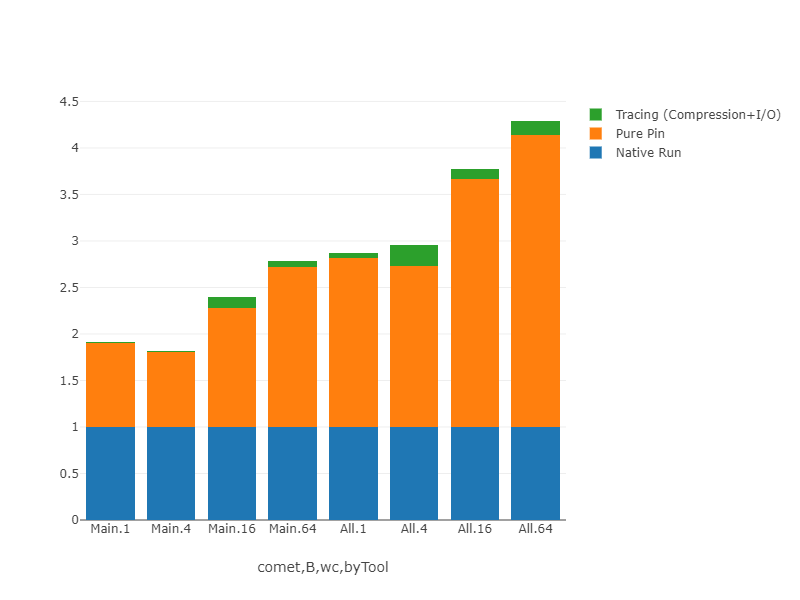
\includegraphics[width=4in]{figs.comet/comet_chartDet_B_wc_byTool_p3_5.png}
\caption{ Input: \textbf{B} - This figure and figure \ref{comet_chartDet_C_wc_byTool_p3_5} shows how much of the overhead of \parlot is caused by \pin and its initialization and how much by that section of \parlot that collects traces and compress them. It seems that overhead added by pure \pin does not scale well and increases with growing number of cores.
}
\label{comet_chartDet_B_wc_byTool_p3_5}
\end{figure}


%Figure c wc
\begin{figure}[!t]
\centering
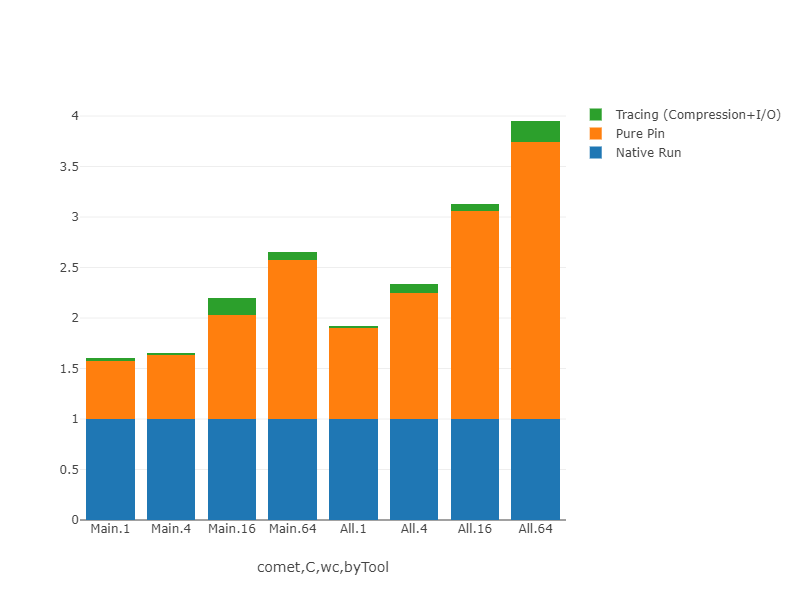
\includegraphics[width=4in]{figs.comet/comet_chartDet_C_wc_byTool_p3_5.png}
\caption{ Input: \textbf{C}
}
\label{comet_chartDet_C_wc_byTool_p3_5}
\end{figure}





\begin{figure}[!t]
\centering
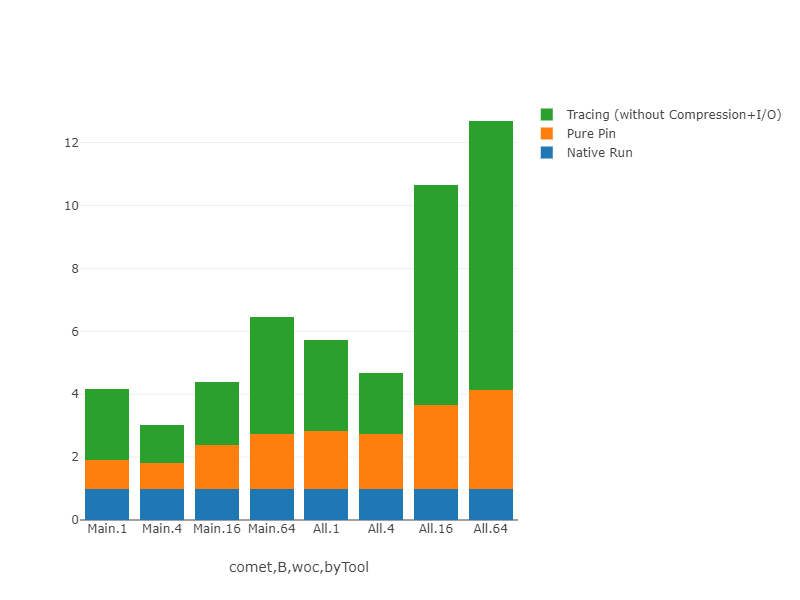
\includegraphics[width=4in]{figs.comet/comet_chartDet_B_woc_byTool_p3_5.png}
\caption{ Input: \textbf{B}- This figure and figure \ref{comet_chartDet_C_woc_byTool_p3_5} shows the impact of \parlot 's data compression. By looking at and comparing green bars of figure \ref{comet_chartDet_B_wc_byTool_p3_5} and \ref{comet_chartDet_B_woc_byTool_p3_5}, clearly it is obvious that how much compressing data improves the performance.
}
\label{comet_chartDet_B_woc_byTool_p3_5}
\end{figure}

\begin{figure}[!t]
\centering
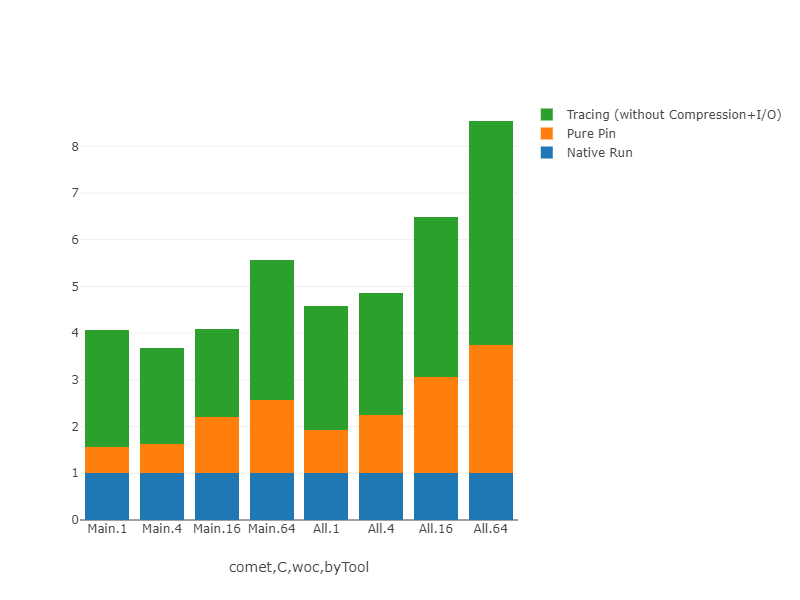
\includegraphics[width=4in]{figs.comet/comet_chartDet_C_woc_byTool_p3_5.png}
\caption{ Input: \textbf{C}
}
\label{comet_chartDet_C_woc_byTool_p3_5}
\end{figure}








\begin{figure}[!t]
\centering
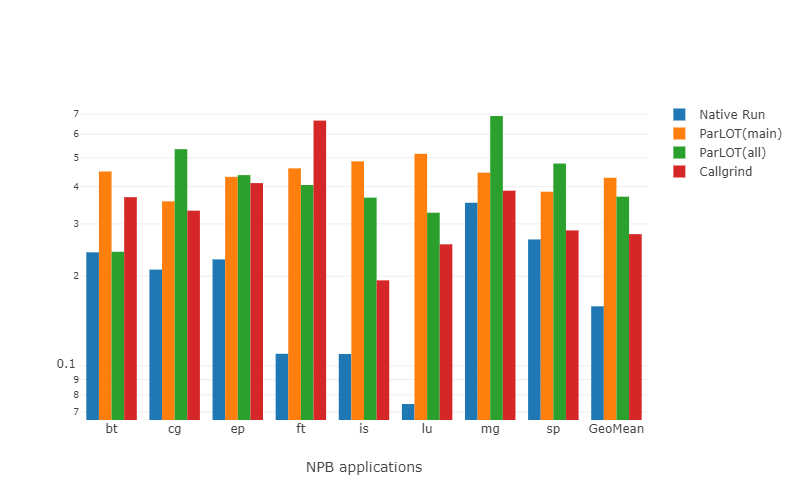
\includegraphics[width=4in]{figs.comet/comet_chartAvg_serr_B_p3_5.png}
\caption{ Input: \textbf{B}  - Standard Error of 3 Runtimes
}
\label{comet_chartAvg_serr_B_p3_5}
\end{figure}




\begin{figure}[!t]
\centering
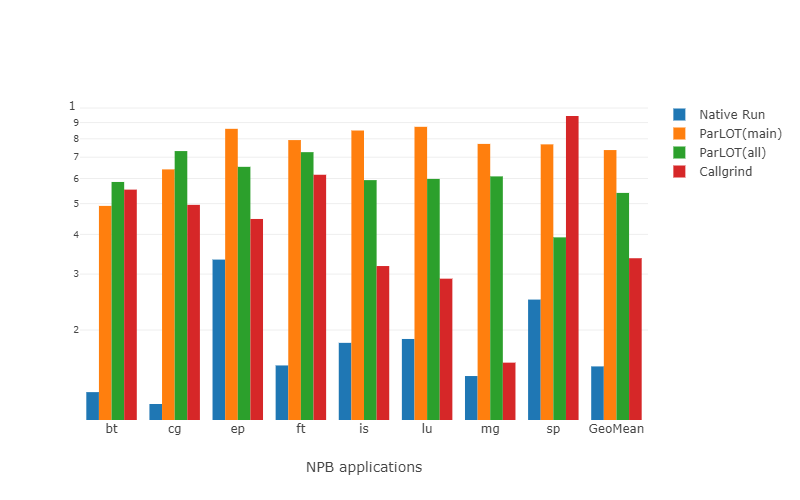
\includegraphics[width=4in]{figs.comet/comet_chartAvg_serr_C_p3_5.png}
\caption{ Input: \textbf{C}  - Standard Error of 3 Runtimes
}
\label{comet_chartAvg_serr_C_p3_5}
\end{figure}





\begin{figure}[!t]
\centering
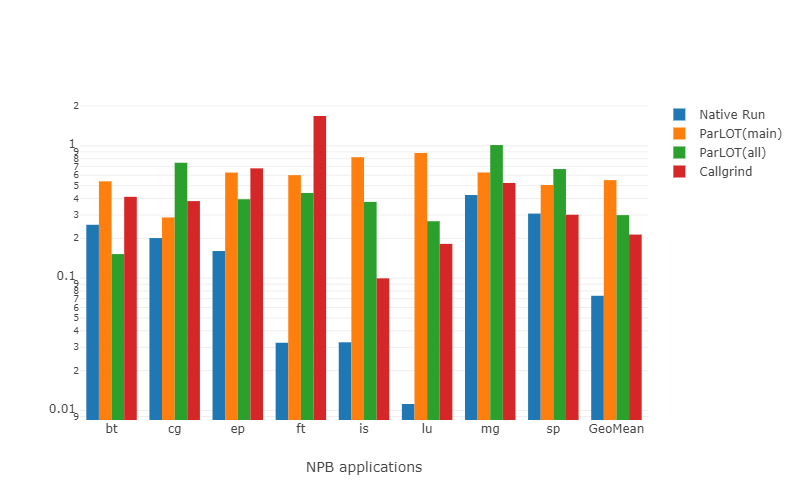
\includegraphics[width=4in]{figs.comet/comet_chartAvg_var_B_p3_5.png}
\caption{ Input: \textbf{B}  - Variance of 3 Runtimes
}
\label{comet_chartAvg_var_B_p3_5}
\end{figure}


\begin{figure}[!t]
\centering
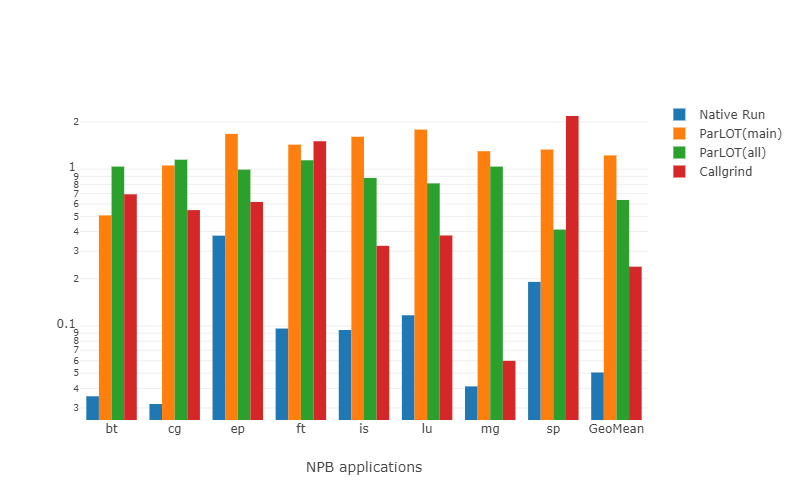
\includegraphics[width=4in]{figs.comet/comet_chartAvg_var_C_p3_5.png}
\caption{ Input: \textbf{C}  - Variance of 3 Runtimes
}
\label{comet_chartAvg_var_C_p3_5}
\end{figure}

%%%%%%%%%%%%%%%%%%%%%%%%%%%%%%%%%%%%%
% Tracing Overhead
%%%%%%%%%%%%%%%%%%%%%%%%%%%%%%%%%%%%%

\subsection{Tracing Overhead}
\label{subsec:lowtoh}
\iffalse

\begin{table*}[]
\caption{Req BW}
\label{comet_bw_pMpAcg_BC_itn_p3.5}\begin{center}
\begin{tabular}{lrrrrrrrrr}
\hline
                &    bt &     cg &    ep &    ft &    is &     lu &    mg &     sp &    GM \\
\hline
 pinMain.B.1    &  4.72 &  21.86 &  3.83 &  1.52 &  0.79 &   2.39 &  5.62 &   5.36 &  3.69 \\
 pinMain.B.4    & 14.28 &  41.08 &  1.89 &  3.48 &  2.24 &  21.48 &  6.45 &  15.85 &  8.12 \\
 pinMain.B.16   & 14.31 &  46.59 &  1.45 &  4.86 &  3.40 &  31.79 &  6.53 &  18.55 &  9.41 \\
 pinMain.B.64   & 18.56 &  43.59 &  1.25 &  4.56 &  4.49 &  27.07 &  5.63 &  29.62 &  9.92 \\
 AVG            & 12.97 &  38.28 &  2.10 &  3.60 &  2.73 &  20.68 &  6.06 &  17.35 &  7.79 \\
 pinAll.B.1     & 48.71 &  89.39 & 47.23 & 45.63 & 59.98 &  53.62 & 60.81 &  54.33 & 56.21 \\
 pinAll.B.4     & 61.84 & 101.23 & 45.21 & 55.12 & 53.20 &  71.09 & 54.85 &  73.62 & 62.68 \\
 pinAll.B.16    & 73.95 & 116.87 & 47.37 & 48.88 & 47.79 & 100.91 & 55.80 &  84.61 & 67.97 \\
 pinAll.B.64    & 81.80 & 110.15 & 44.16 & 47.98 & 37.84 & 100.26 & 52.67 &  99.90 & 66.47 \\
 AVG            & 66.58 & 104.41 & 45.99 & 49.40 & 49.70 &  81.47 & 56.03 &  78.12 & 63.33 \\
 callgrind.B.1  &  1.57 &   7.69 &  7.39 &  4.56 & 39.49 &   2.61 & 34.41 &   2.71 &  6.67 \\
 callgrind.B.4  &  6.51 &  16.01 & 22.10 & 15.65 & 45.46 &   8.63 & 45.47 &   7.78 & 16.31 \\
 callgrind.B.16 & 17.20 &  24.62 & 37.42 & 23.84 & 29.87 &  16.23 & 51.49 &  15.81 & 24.93 \\
 callgrind.B.64 & 26.82 &  27.65 & 45.93 & 25.14 & 11.04 &  17.75 & 45.27 &  20.20 & 25.02 \\
 AVG            & 13.03 &  18.99 & 28.21 & 17.30 & 31.47 &  11.30 & 44.16 &  11.62 & 18.23 \\
 pinMain.C.1    &  1.82 &  16.96 &  5.15 &  1.16 &  0.69 &   0.77 &  3.56 &   1.40 &  2.17 \\
 pinMain.C.4    &  7.53 &  44.87 &  3.00 &  2.50 &  2.12 &  20.13 &  7.08 &  13.74 &  7.55 \\
 pinMain.C.16   & 16.30 &  55.04 &  1.84 &  6.10 &  3.35 &  34.09 &  7.24 &  20.68 & 10.70 \\
 pinMain.C.64   & 17.45 &  61.43 &  1.30 &  5.93 &  4.42 &  38.28 &  5.62 &  26.09 & 10.94 \\
 AVG            & 10.77 &  44.58 &  2.82 &  3.92 &  2.65 &  23.32 &  5.88 &  15.48 &  7.84 \\
 pinAll.C.1     & 17.80 &  53.37 & 26.34 & 20.89 & 48.31 &  25.31 & 52.61 &  19.46 & 29.99 \\
 pinAll.C.4     & 51.78 &  95.84 & 36.80 & 43.82 & 51.40 &  58.39 & 54.18 &  65.77 & 55.15 \\
 pinAll.C.16    & 75.38 & 121.03 & 44.29 & 61.39 & 46.90 & 101.05 & 56.49 & 101.32 & 71.37 \\
 pinAll.C.64    & 80.63 & 135.19 & 43.49 & 46.28 & 37.09 & 117.87 & 54.05 &  99.02 & 68.99 \\
 AVG            & 56.40 & 101.36 & 37.73 & 43.09 & 45.93 &  75.66 & 54.33 &  71.39 & 56.38 \\
 callgrind.C.1  &  0.40 &   3.09 &  1.96 &  1.05 & 14.60 &   0.70 &  6.96 &   0.75 &  1.85 \\
 callgrind.C.4  &  1.78 &   8.87 &  7.74 &  4.48 & 31.74 &   2.82 & 21.03 &   2.78 &  6.41 \\
 callgrind.C.16 &  6.01 &  15.82 & 22.86 & 10.75 & 26.50 &   7.45 & 39.05 &   6.96 & 13.72 \\
 callgrind.C.64 & 14.32 &  19.56 & 35.75 & 12.17 & 11.07 &  11.86 & 40.69 &  12.83 & 17.39 \\
 AVG            &  5.63 &  11.84 & 17.08 &  7.11 & 20.98 &   5.71 & 26.93 &   5.83 &  9.84 \\
\hline
\end{tabular}
\end{center}
\end{table*}

\fi


\iftrue

\begin{table*}[]
\caption{ Required Bandwidth per core (kB/s) }
\label{comet_bw_pMpAcg_BC_itn_p3.5}\begin{center}
\npdecimalsign{.}
\nprounddigits{1}

\begin{tabular}{|c|c|c|n{3}{1}n{3}{1}n{3}{1}n{3}{1}n{3}{1}n{3}{1}n{3}{1}n{3}{1}|n{3}{1}|}
\hline
Input & Tool & \# Nodes  & \multicolumn{1}{c}{bt} & \multicolumn{1}{c}{cg} & \multicolumn{1}{c}{ep} & \multicolumn{1}{c}{ft} & \multicolumn{1}{c}{is} & \multicolumn{1}{c}{lu} & \multicolumn{1}{c}{mg} & \multicolumn{1}{c|}{sp} & \multicolumn{1}{c|}{GM} \\ \hline
\multirow{15}{*}{B} & \multirow{5}{*}{ParLOT(m)} & 1 &  4.72 &  21.86 &  3.83 &  1.52 &  0.79 &   2.39 &  5.62 &   5.36 &  3.69 \\
 & & 4                                               & 14.28 &  41.08 &  1.89 &  3.48 &  2.24 &  21.48 &  6.45 &  15.85 &  8.12 \\
 & & 16                                              & 14.31 &  46.59 &  1.45 &  4.86 &  3.40 &  31.79 &  6.53 &  18.55 &  9.41 \\
 & & 64                                              & 18.56 &  43.59 &  1.25 &  4.56 &  4.49 &  27.07 &  5.63 &  29.62 &  9.92 \\ \cline{3-12} 
 & & AVG                                             & 12.97 &  38.28 &  2.10 &  3.60 &  2.73 &  20.68 &  6.06 &  17.35 &  {\boldmath}7.79  \\ \cline{2-12} 
 & \multirow{5}{*}{ParLOT(a)} & 1 & 48.71 &  89.39 & 47.23 & 45.63 & 59.98 &  53.62 & 60.81 &  54.33 & 56.21 \\
 & & 4                            & 61.84 & 101.23 & 45.21 & 55.12 & 53.20 &  71.09 & 54.85 &  73.62 & 62.68 \\
 & & 16                           & 73.95 & 116.87 & 47.37 & 48.88 & 47.79 & 100.91 & 55.80 &  84.61 & 67.97 \\
 & & 64                           & 81.80 & 110.15 & 44.16 & 47.98 & 37.84 & 100.26 & 52.67 &  99.90 & 66.47 \\ \cline{3-12} 
 & & AVG                          & 66.58 & 104.41 & 45.99 & 49.40 & 49.70 &  81.47 & 56.03 &  78.12 & {\boldmath}63.33 \\ \cline{2-12} 
 & \multirow{5}{*}{Callgrind}  & 1  &  1.57 &   7.69 &  7.39 &  4.56 & 39.49 &   2.61 & 34.41 &   2.71 &  6.67  \\
 & & 4                              &  6.51 &  16.01 & 22.10 & 15.65 & 45.46 &   8.63 & 45.47 &   7.78 & 16.31  \\
 & & 16                             & 17.20 &  24.62 & 37.42 & 23.84 & 29.87 &  16.23 & 51.49 &  15.81 & 24.93  \\
 & & 64                             & 26.82 &  27.65 & 45.93 & 25.14 & 11.04 &  17.75 & 45.27 &  20.20 & 25.02  \\ \cline{3-12} 
 & & AVG                            & 13.03 &  18.99 & 28.21 & 17.30 & 31.47 &  11.30 & 44.16 &  11.62 & {\boldmath}18.23  \\ \hline
 \multirow{15}{*}{C} & \multirow{5}{*}{ParLOT(m)} & 1  &  1.82 &  16.96 &  5.15 &  1.16 &  0.69 &   0.77 &  3.56 &   1.40 &  2.17  \\
 & & 4                                                 &  7.53 &  44.87 &  3.00 &  2.50 &  2.12 &  20.13 &  7.08 &  13.74 &  7.55  \\
 & & 16                                                & 16.30 &  55.04 &  1.84 &  6.10 &  3.35 &  34.09 &  7.24 &  20.68 & 10.70  \\
 & & 64                                                & 17.45 &  61.43 &  1.30 &  5.93 &  4.42 &  38.28 &  5.62 &  26.09 & 10.94  \\ \cline{3-12} 
 & & AVG                                               & 10.77 &  44.58 &  2.82 &  3.92 &  2.65 &  23.32 &  5.88 &  15.48 &  {\boldmath}7.84  \\ \cline{2-12} 
 & \multirow{5}{*}{ParLOT(a)} & 1 & 17.80 &  53.37 & 26.34 & 20.89 & 48.31 &  25.31 & 52.61 &  19.46 & 29.99 \\
 & & 4                            & 51.78 &  95.84 & 36.80 & 43.82 & 51.40 &  58.39 & 54.18 &  65.77 & 55.15 \\
 & & 16                           & 75.38 & 121.03 & 44.29 & 61.39 & 46.90 & 101.05 & 56.49 & 101.32 & 71.37 \\
 & & 64                           & 80.63 & 135.19 & 43.49 & 46.28 & 37.09 & 117.87 & 54.05 &  99.02 & 68.99 \\ \cline{3-12}
 & & AVG                          & 56.40 & 101.36 & 37.73 & 43.09 & 45.93 &  75.66 & 54.33 &  71.39 & {\boldmath}56.38  \\ \cline{2-12} 
 & \multirow{5}{*}{Callgrind} & 1 &  0.40 &   3.09 &  1.96 &  1.05 & 14.60 &   0.70 &  6.96 &   0.75 &  1.85  \\
 & & 4                            &  1.78 &   8.87 &  7.74 &  4.48 & 31.74 &   2.82 & 21.03 &   2.78 &  6.41  \\
 & & 16                           &  6.01 &  15.82 & 22.86 & 10.75 & 26.50 &   7.45 & 39.05 &   6.96 & 13.72  \\
 & & 64                           & 14.32 &  19.56 & 35.75 & 12.17 & 11.07 &  11.86 & 40.69 &  12.83 & 17.39  \\ \cline{3-12}
 & & AVG                          &  5.63 &  11.84 & 17.08 &  7.11 & 20.98 &   5.71 & 26.93 &   5.83 &  {\boldmath}9.84  \\ \hline
\end{tabular}
\end{center}
\end{table*}

\fi


%%%%%%%%%%%%%%%%%%%%%%%%%%%%%%%%%
% FROM RESULTS - average bandwidth
%%%%%%%%%%%%%%%%%%%%%%%%%%%%%%%%%
\begin{figure}[t]
\centering
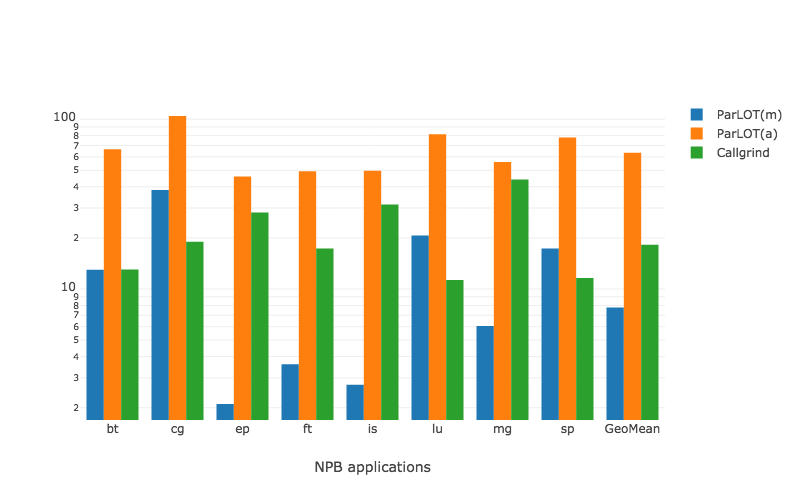
\includegraphics[width=3.4in,height=1.9in]{figs.comet.newMed/comet_chartAvg_bw_B_p3_5.png}
\caption{  Average required bandwidth per core (kB/s) on the NPB applications - Input B}
\label{comet_chartAvg_bw_B_p3_5}
\end{figure}

\begin{figure}[t]
\centering
\includegraphics[width=3.4in,height=1.9in]{figs.comet.newMed/comet_chartAvg_bw_C_p3_5.png}
\caption{ Average required bandwidth per core (kB/s) on the NPB applications - Input C}
\label{comet_chartAvg_bw_C_p3_5}
\end{figure}

%%%%%%%%%%%%%%%%%%%%%%%%%%%%%%%%%
% ENDDDD
%%%%%%%%%%%%%%%%%%%%%%%%%%%%%%%%%

Table \ref{comet_sd_pMpAcg_BC_itn_p3.5} shows the tracing overhead of \parlotm, \parlota, and \callgrind on each application of the NPB benchmark suite for different node counts. The last column of the table lists the geometric mean over all eight programs. The AVG rows show the average over the four node counts.


On average, both \parlotm and \parlota outperform \callgrind. The bolded numbers in Table \ref{comet_sd_pMpAcg_BC_itn_p3.5} for input C show that the average overhead is 1.94 for \parlotm, 2.73 for \parlota, and 4.63 for \callgrind. Figures \ref{comet_chartAvg_sd_B_p3_5} and \ref{comet_chartAvg_sd_C_p3_5} show these results in visual form.


The key takeaway point is that the overhead of \parlot is roughly a factor of two to three, which we believe users may be willing to accept, for example, if it helps them debug their applications. This is very promising especially when considering how detailed the collected trace information is and that most of the overhead is due to \pin (see \S\ref{subsec:pinit}. Note that \parlot 's overhead is typically lower than that of \callgrind, which collects less information.

The overhead of \parlot increases as we scale the applications to more compute nodes. However, the increase is quite small. Going from 16 to 1024 cores, a 64-fold increase in parallelism, only increases the average overhead by between 1.3- and 2.1-fold. In contrast, \callgrind 's overhead decreases with increasing node count, making it more scalable. Having said that, \callgrind 's overhead is larger for the C inputs whereas \parlot 's overhead is larger for the smaller B inputs. In other words, \parlot scales better to larger inputs than \callgrind.

\parlot 's scaling behavior can be explained by correlating it with the expected function-call frequency. When distributing a fixed problem size over more cores, each core receives less work. As a consequence, less time is spent in the functions that process the work, resulting in more function calls per time unit, which causes more work for \parlot. In contrast, when distributing a larger problem size over the same number of cores, each core receives more work. Hence, more time is spent in the functions that process the work, resulting in fewer function calls per time unit, which causes less work for \parlot and therefore less tracing overhead. Hence, we believe \parlot 's overhead to be even lower on long-running inputs, which is where our tracing technique is needed the most.


In summary, \parlot 's overhead is in the single digits for all evaluated applications and configurations, including for 1024-core runs. It appears to scale reasonably to larger node counts and well to larger problem sizes.
  
\subsection{Required Bandwidth}
\label{subsec:lowbw}

Table \ref{comet_bw_pMpAcg_BC_itn_p3.5}, Fig.  \ref{comet_chartAvg_bw_B_p3_5} and Fig. \ref{comet_chartAvg_bw_C_p3_5} show how much trace bandwidth each tool 
requires
during the application execution. 
%
On average, \parlotm requires less bandwidth than
\callgrind, especially for smaller inputs. 
%
\parlota's bandwidth is much higher as it collects call info from all
images, and not just the main image than that of \parlotm.

We see that the required bandwidth for different input sizes of the NPB applications are almost equal in \parlot. According to NPB documentation, number of iterations in both input B and C are the same for all applications and their difference is the number of elements or the grid size. It is clear that the required bandwidth of \parlot is independent of the problem size, unlike \callgrind, where the input size has linear impact on results.

%
%%%%%%%%%%%%%%%%%%%%%%%%%%%%%%%%%
% FROM RESULTS - average compression ratio
%%%%%%%%%%%%%%%%%%%%%%%%%%%%%%%%%
\begin{figure}[t]
\centering
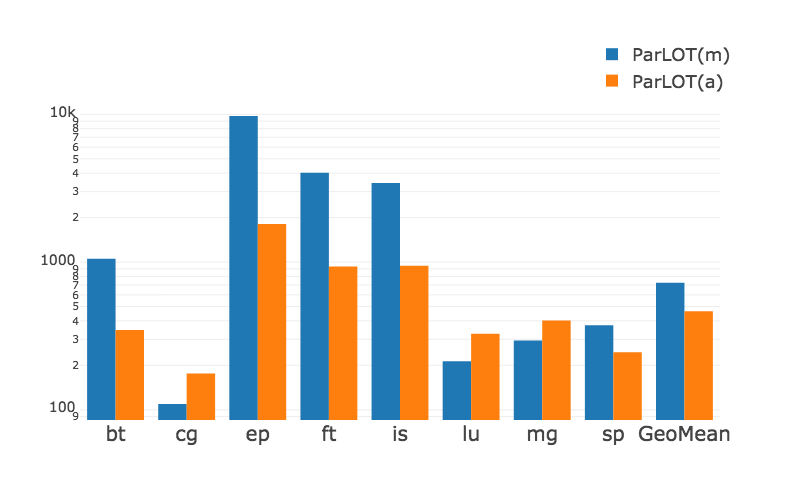
\includegraphics[width=3.2in,height=1.9in]{figs.comet.newMed/comet_chartAvg_cr_B_p3_5.png}
\caption{ Average compression ratio of \parlot on the NPB applications - Input B}
\label{comet_chartAvg_cr_B_p3_5}
\end{figure}

\begin{figure}[t]
\centering
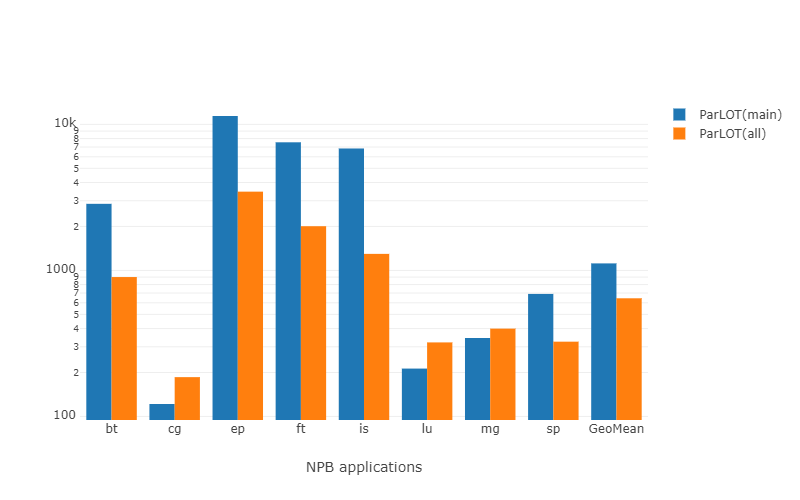
\includegraphics[width=3.2in,height=1.9in]{figs.comet.newMed/comet_chartAvg_cr_C_p3_5.png}
\caption{ Average compression ratio of \parlot on the NPB applications - Input C}
\label{comet_chartAvg_cr_C_p3_5}
\end{figure}
%%%%%%%%%%%%%%%%%%%%%%%%%%%%%%%%%
% ENDDDD
%%%%%%%%%%%%%%%%%%%%%%%%%%%%%%%%%



\iffalse
\begin{table*}[]
\caption{Compression Ratio}
\label{comet_cr_pMpA_BC_itn_p3.5}\begin{center}
\begin{tabular}{lrrrrrrrrr}
\hline
              &      bt &     cg &       ep &       ft &       is &     lu &     mg &      sp &      GM \\
\hline
 pinMain.B.1  & 3035.93 &  94.35 & 12456.18 & 12173.49 &  9718.38 & 167.72 &  99.08 &  878.27 & 1255.17 \\
 pinMain.B.4  &  586.64 &  82.48 & 10368.41 &  1737.09 &   909.20 & 140.29 & 254.95 &  338.16 &  559.36 \\
 pinMain.B.16 &  346.66 & 113.28 &  8563.85 &  1077.35 &  1200.57 & 178.98 & 387.63 &  123.02 &  496.83 \\
 pinMain.B.64 &  252.24 & 147.78 &  7611.04 &  1122.62 &  1907.95 & 366.80 & 437.31 &  152.91 &  591.11 \\
 AVG          & 1055.37 & 109.47 &  9749.87 &  4027.64 &  3434.03 & 213.45 & 294.74 &  373.09 &  725.62 \\
 pinAll.B.1   &  514.51 & 137.41 &  3335.77 &  1226.74 &   543.18 & 314.63 & 260.87 &  303.88 &  500.21 \\
 pinAll.B.4   &  315.71 & 137.21 &  1266.92 &   436.15 &   316.16 & 287.25 & 329.57 &  199.66 &  330.70 \\
 pinAll.B.16  &  226.86 & 181.58 &  1246.66 &  1026.53 &   927.09 & 299.30 & 469.29 &  171.52 &  430.39 \\
 pinAll.B.64  &  329.23 & 247.30 &  1394.07 &  1043.94 &  1984.62 & 410.32 & 548.47 &  307.16 &  597.55 \\
 AVG          &  346.58 & 175.88 &  1810.86 &   933.34 &   942.76 & 327.88 & 402.05 &  245.56 &  464.71 \\
 pinMain.C.1  & 8618.95 & 111.16 & 13067.96 & 21335.57 & 21856.49 & 350.03 & 247.44 & 1977.43 & 2371.35 \\
 pinMain.C.4  & 1910.64 & 110.45 & 12418.66 &  6520.34 &  2256.56 & 112.77 & 267.98 &  472.68 &  928.16 \\
 pinMain.C.16 &  580.79 & 133.24 & 11017.36 &  1239.31 &  1347.88 & 164.47 & 396.86 &  143.13 &  582.78 \\
 pinMain.C.64 &  322.83 & 131.92 &  9154.99 &  1065.12 &  1896.25 & 223.69 & 465.74 &  168.89 &  585.74 \\
 AVG          & 2858.30 & 121.69 & 11414.74 &  7540.09 &  6839.30 & 212.74 & 344.50 &  690.53 & 1117.01 \\
 pinAll.C.1   & 2579.37 & 181.76 &  7376.96 &  5143.08 &  1520.42 & 408.21 & 314.77 &  650.73 & 1107.37 \\
 pinAll.C.4   &  448.61 & 161.32 &  3194.58 &  1062.94 &   527.34 & 274.70 & 319.35 &  237.43 &  477.42 \\
 pinAll.C.16  &  285.05 & 185.74 &  1765.49 &   588.86 &  1106.34 & 273.63 & 467.35 &  141.69 &  426.92 \\
 pinAll.C.64  &  290.00 & 214.68 &  1512.89 &  1237.30 &  2038.72 & 329.04 & 496.21 &  270.83 &  565.82 \\
 AVG          &  900.76 & 185.88 &  3462.48 &  2008.05 &  1298.21 & 321.39 & 399.42 &  325.17 &  644.38 \\
\hline
\end{tabular}
\end{center}
\end{table*}

\fi


\iftrue

\begin{table*}[]
\caption{ Compression ratio }
\label{comet_cr_pMpA_BC_itn_p3.5}\begin{center}
\npdecimalsign{.}
\nprounddigits{1}
\begin{tabular}{|c|c|c|N{5}{1}N{5}{1}N{5}{1}N{5}{1}N{5}{1}N{5}{1}n{5}{1}n{5}{1}|n{5}{1}|}
\hline
Input & Tool & \# Nodes  & \multicolumn{1}{c}{bt} & \multicolumn{1}{c}{cg} & \multicolumn{1}{c}{ep} & \multicolumn{1}{c}{ft} & \multicolumn{1}{c}{is} & \multicolumn{1}{c}{lu} & \multicolumn{1}{c}{mg} & \multicolumn{1}{c|}{sp} & \multicolumn{1}{c|}{GM} \\ \hline
\multirow{10}{*}{B} & \multirow{5}{*}{ParLOT(m)} & 1 & 3035.93 &  94.35 & 12456.18 & 12173.49 &  9718.38 & 167.72 &  99.08 &  878.27 & 1255.17 \\
 & & 4                                               &  586.64 &  82.48 & 10368.41 &  1737.09 &   909.20 & 140.29 & 254.95 &  338.16 &  559.36 \\
 & & 16                                              &  346.66 & 113.28 &  8563.85 &  1077.35 &  1200.57 & 178.98 & 387.63 &  123.02 &  496.83 \\
 & & 64                                              &  252.24 & 147.78 &  7611.04 &  1122.62 &  1907.95 & 366.80 & 437.31 &  152.91 &  591.11 \\ \cline{3-12} 
 & & AVG                                             & 1055.37 & 109.47 &  9749.87 &  4027.64 &  3434.03 & 213.45 & 294.74 &  373.09 &  {\boldmath}725.62  \\ \cline{2-12} 
 & \multirow{5}{*}{ParLOT(a)} & 1 &  514.51 & 137.41 &  3335.77 &  1226.74 &   543.18 & 314.63 & 260.87 &  303.88 &  500.21 \\
 & & 4                            &  315.71 & 137.21 &  1266.92 &   436.15 &   316.16 & 287.25 & 329.57 &  199.66 &  330.70 \\
 & & 16                           &  226.86 & 181.58 &  1246.66 &  1026.53 &   927.09 & 299.30 & 469.29 &  171.52 &  430.39 \\
 & & 64                           &  329.23 & 247.30 &  1394.07 &  1043.94 &  1984.62 & 410.32 & 548.47 &  307.16 &  597.55 \\ \cline{3-12} 
 & & AVG                          &  346.58 & 175.88 &  1810.86 &   933.34 &   942.76 & 327.88 & 402.05 &  245.56 &  {\boldmath}464.71 \\ \hline 
 \multirow{10}{*}{C} & \multirow{5}{*}{ParLOT(m)} & 1  & 8618.95 & 111.16 & 13067.96 & 21335.57 & 21856.49 & 350.03 & 247.44 & 1977.43 & 2371.35  \\
 & & 4                                                 & 1910.64 & 110.45 & 12418.66 &  6520.34 &  2256.56 & 112.77 & 267.98 &  472.68 &  928.16  \\
 & & 16                                                &  580.79 & 133.24 & 11017.36 &  1239.31 &  1347.88 & 164.47 & 396.86 &  143.13 &  582.78  \\
 & & 64                                                &  322.83 & 131.92 &  9154.99 &  1065.12 &  1896.25 & 223.69 & 465.74 &  168.89 &  585.74  \\ \cline{3-12} 
 & & AVG                                               & 2858.30 & 121.69 & 11414.74 &  7540.09 &  6839.30 & 212.74 & 344.50 &  690.53 & {\boldmath}1117.01  \\ \cline{2-12} 
 & \multirow{5}{*}{ParLOT(a)} & 1 & 2579.37 & 181.76 &  7376.96 &  5143.08 &  1520.42 & 408.21 & 314.77 &  650.73 & 1107.37 \\
 & & 4                            &  448.61 & 161.32 &  3194.58 &  1062.94 &   527.34 & 274.70 & 319.35 &  237.43 &  477.42 \\
 & & 16                           &  285.05 & 185.74 &  1765.49 &   588.86 &  1106.34 & 273.63 & 467.35 &  141.69 &  426.92 \\
 & & 64                           &  290.00 & 214.68 &  1512.89 &  1237.30 &  2038.72 & 329.04 & 496.21 &  270.83 &  565.82 \\ \cline{3-12}
 & & AVG                          &  900.76 & 185.88 &  3462.48 &  2008.05 &  1298.21 & 321.39 & 399.42 &  325.17 &  {\boldmath}644.38 \\ \cline{2-12} \hline
\end{tabular}
\npnoround
\end{center}
\end{table*}

\fi





\begin{figure}[t]
\centering
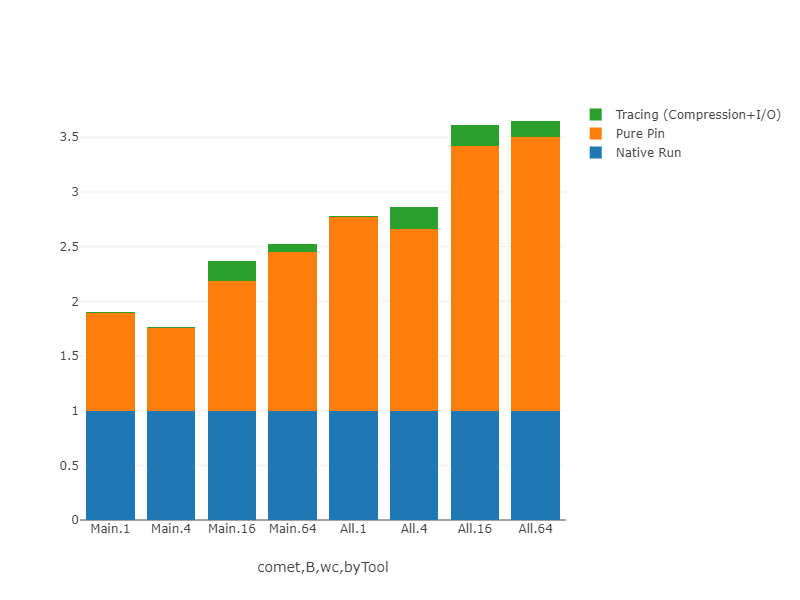
\includegraphics[width=3.1in,height=1.9in]{figs.comet.newMed/comet_chartDet_B_wc_byTool_p3_5.png}
\caption{ Tracing overhead breakdown - Input B}
\label{comet_chartDet_B_wc_byTool_p3_5}
\end{figure}


\begin{figure}[t]
\centering
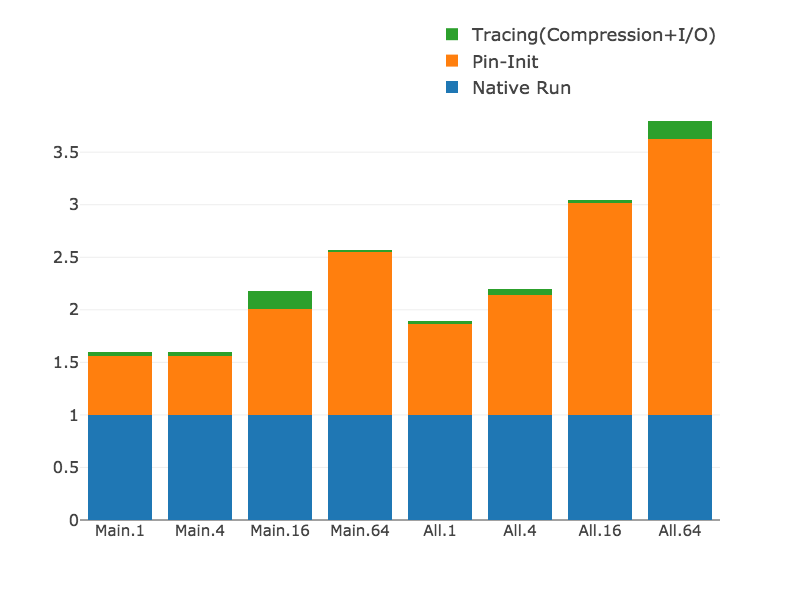
\includegraphics[width=3.1in,height=1.9in]{figs.comet.newMed/comet_chartDet_C_wc_byTool_p3_5.png}
\caption{ Tracing overhead breakdown - Input C}
\label{comet_chartDet_C_wc_byTool_p3_5}
\end{figure}



\begin{figure}[t]
\centering
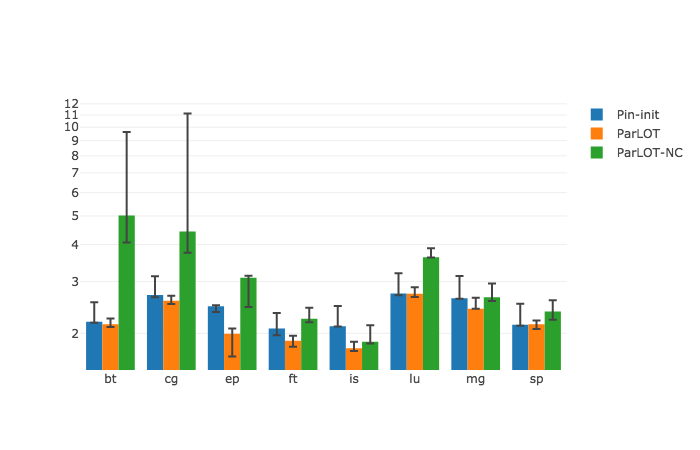
\includegraphics[width=3.2in,height=1.9in]{figs.comet.newMed/comet_BX2_Main_16_B_p3_5.png}
\caption{ Variability of \parlotm overhead on 16 nodes - Input B}
\label{comet_BX2_Main_16_B_p3_5}
\end{figure}


%%%%%%%%%%%%%%%%%%%%%%%%%%%%%%%%%%%%%%%%%%%%%%%%%%%%%%%%%%%%%%%%%%%%%%%%%%%%%%%%%%
  
\subsection{Compression Ratio}
\label{subsec:cr}
Table \ref{comet_cr_pMpA_BC_itn_p3.5} shows the compression ratios for all configurations and inputs.
%
On average, \parlot stores between half a kilobyte and a kilobyte of trace info in a single byte. 
%
We observe that the
average compression ratio for \parlota input C is 644.3, and its
corresponding required bandwidth from Table
\ref{comet_bw_pMpAcg_BC_itn_p3.5} is 56.3.
%
This means \parlot can
collect \textbf{more than 36 MB} worth of data per core per second
while only needing 56 kB/s of the system bandwidth, {\em leaving the rest of the available bandwidth for application.}
%
In comparison, \callgrind only
collects \textbf{less than 100 kB} of data but still adds more
overhead compared to either \parlota or \parlotm . 
%
The average amount of trace data that can be collected by \parlota is
\textbf{360x} (85x for \parlotm) larger than that for \callgrind.
%
In the best observed case, the compression ratio of
\parlot exceeds 21000.
%
This is particularly impressive because it was achieved with relatively low overhead and incremental  
on-the-fly compression.
%
Generally, the compression ratios of \parlotm are higher than those of \parlota because the variety of distinct function calls on the main image is smaller than when tracing all images, thus compression performs better on \parlotm. 
Also by looking at Fig. \ref{comet_chartAvg_bw_B_p3_5}, Fig. \ref{comet_chartAvg_bw_C_p3_5}, Fig. \ref{comet_chartAvg_cr_B_p3_5} and Fig. \ref{comet_chartAvg_cr_C_p3_5}, we find EP to have the maximum compression ratio among the NPB applications. At the same time, it has the minimum required bandwidth. The opposite is true for CG, which exhibits the minimum compression ratio and the maximum required bandwidth. CG is a conjugate gradient method with irregular memory accesses and communications whereas EP is an embarrassingly parallel random number generator. CG's whole-program trace contains a larger number of distinct calls and more complex patterns than that of EP, thus resulting in a higher bandwidth and smaller compression ratio.
%

\parlot's ompression mechanism works better on larger input sizes because larger inputs tend to result in longer streams of similar function calls (e.g., a call that is made for every processed element)
  

  
\subsection{Overheads} 
\label{subsec:pinit}
Tables \ref{comet_wo_det_Main_all_B_p3.5} and
\ref{comet_wo_det_All_all_B_p3.5} present the average overhead added on each
application for different versions of \parlot. 
%
The last row of these two tables
presents the geometric mean.
%
This information captures how much each
phase of \parlot slows down the native execution. 

\begin{table*}[]
\caption{Tracing overhead added by each version of \parlot - Input: B}
\begin{center}
\label{comet_wo_det_Main_all_B_p3.5}
\scalebox{0.80}{
\begin{tabular}{|c|c|rrr|rrr|rrr|rrr|} 
\hline 
\multicolumn{1}{|l|}{\multirow{2}{*}{\textbf{Input: B}}} & \multicolumn{1}{r|}{Nodes :}    & \multicolumn{3}{c|}{1}  & \multicolumn{3}{c|}{4} & \multicolumn{3}{c|}{16}  & \multicolumn{3}{c|}{64} \\ \cline{2-14} 
\multicolumn{1}{|l|}{} & \multicolumn{1}{r|}{Detail Tools:} & \multicolumn{1}{c}{\pininit} & \multicolumn{1}{c}{\parlot} & \multicolumn{1}{c|}{\parlotnc} & \multicolumn{1}{c}{\pininit} & \multicolumn{1}{c}{\parlot} & \multicolumn{1}{c|}{\parlotnc} & \multicolumn{1}{c}{\pininit} & \multicolumn{1}{c}{\parlot} & \multicolumn{1}{c|}{\parlotnc} & \multicolumn{1}{c}{\pininit} & \multicolumn{1}{c}{\parlot} & \multicolumn{1}{c|}{\parlotnc} \\
\hline
\multirow{9}{*}{Main} &  bt  &  1.50  &  1.55  &   5.62  &  1.74  &  1.76  &  5.06  &  2.19  & \cellcolor{blue!25} 2.15  &  5.02  &  1.83  &  2.10  &  3.52 \\
 &  cg  &  1.75  &  1.82  &   2.38  &  1.84  &  1.85  &  2.64  &  2.70  & \cellcolor{blue!25} 2.58  &  4.43  &  2.32  & \cellcolor{blue!25} 2.17  &  4.64 \\
 &  ep  &  2.96  & \cellcolor{blue!25} 2.62  &  20.48  &  1.99  & \cellcolor{blue!25} 1.89  &  5.38  &  2.47  & \cellcolor{blue!25} 1.99  &  3.09  &  2.68  & \cellcolor{blue!25} 2.39  &  2.66 \\
 &  ft  &  1.87  &  2.11  &   6.17  &  1.75  & \cellcolor{blue!25} 1.74  &  2.79  &  2.08  & \cellcolor{blue!25} 1.89  &  2.24  &  2.18  & \cellcolor{blue!25} 1.96  &  2.14 \\
 &  is  &  2.47  &  2.47  &   4.82  &  1.79  & \cellcolor{blue!25} 1.78  &  2.07  &  2.11  & \cellcolor{blue!25} 1.78  &  1.87  &  4.51  & \cellcolor{blue!25} 4.31  &  5.71 \\
 &  lu  &  1.32  & \cellcolor{blue!25} 1.31  &   1.44  &  1.75  &  1.77  &  2.25  &  2.73  &  2.73  &  3.62  &  3.05  &  4.39  &  6.13 \\
 &  mg  &  2.56  & \cellcolor{blue!25} 2.53  &   2.79  &  1.56  & \cellcolor{blue!25} 1.52  &  1.59  &  2.63  & \cellcolor{blue!25} 2.43  &  2.65  &  1.95  &  1.97  &  1.85 \\
 &  sp  &  1.34  & \cellcolor{blue!25} 1.33  &   2.43  &  1.73  &  1.73  &  3.58  &  2.14  &  2.15  &  2.37  &  1.95  &  2.07  &  2.54 \\
\cline{2-14}
 &  GM  &  1.89  &  1.90  &   4.10  &  1.77  & \cellcolor{blue!25} 1.75  &  2.92  &  2.37  & \cellcolor{blue!25} 2.19  &  3.00  &  2.45  &  2.52  &  3.33 \\
\hline 
\end{tabular} }

\end{center}
\end{table*}


\begin{table*}[]
\caption{Tracing overhead added by each version of \parlot - Input: B}
\begin{center}
\label{comet_wo_det_All_all_B_p3.5}
\scalebox{0.8}{
\begin{tabular}{|c|c|rrr|rrr|rrr|rrr|} 
\hline 
\multicolumn{1}{|l|}{\multirow{2}{*}{\textbf{Input: B}}} & \multicolumn{1}{r|}{Nodes :}    & \multicolumn{3}{c|}{1}  & \multicolumn{3}{c|}{4} & \multicolumn{3}{c|}{16}  & \multicolumn{3}{c|}{64} \\ \cline{2-14} 
\multicolumn{1}{|l|}{} & \multicolumn{1}{r|}{Detail Tools:} & \multicolumn{1}{c}{\pininit} & \multicolumn{1}{c}{\parlot} & \multicolumn{1}{c|}{\parlotnc} & \multicolumn{1}{c}{\pininit} & \multicolumn{1}{c}{\parlot} & \multicolumn{1}{c|}{\parlotnc} & \multicolumn{1}{c}{\pininit} & \multicolumn{1}{c}{\parlot} & \multicolumn{1}{c|}{\parlotnc} & \multicolumn{1}{c}{\pininit} & \multicolumn{1}{c}{\parlot} & \multicolumn{1}{c|}{\parlotnc} \\
\hline
\multirow{9}{*}{All} &  bt  &  1.76  &  1.84  &   6.11  &  2.39  &  2.57  &  6.11  &  3.22  &  3.52  &   9.02  &  2.87  &  3.14  &   7.55 \\
 &  cg  &  2.69  &  2.73  &   3.80  &  2.86  &  3.06  &  4.48  &  4.07  &  4.20  &  11.38  &  3.33  & \cellcolor{blue!25} 3.26  &  10.39 \\
 &  ep  &  4.36  & \cellcolor{blue!25} 4.18  &  22.20  &  3.14  &  3.41  &  7.16  &  3.12  &  3.39  &   4.55  &  4.18  & \cellcolor{blue!25} 3.83  &   4.16 \\
 &  ft  &  2.80  & \cellcolor{blue!25} 2.78  &   6.85  &  2.65  &  2.77  &  3.82  &  2.82  &  2.94  &   3.66  &  3.15  & \cellcolor{blue!25} 3.02  &   3.57 \\
 &  is  &  4.40  & \cellcolor{blue!25} 4.22  &   7.04  &  2.85  &  2.96  &  3.42  &  2.91  & \cellcolor{blue!25} 2.83  &   3.24  &  5.38  &  5.44  &   8.81 \\
 &  lu  &  1.70  &  1.73  &   2.39  &  2.54  &  2.76  &  4.88  &  3.96  &  4.30  &  10.47  &  4.45  &  4.65  &  23.41 \\
 &  mg  &  4.83  & \cellcolor{blue!25} 4.75  &   5.37  &  2.51  &  2.79  &  3.07  &  4.32  &  4.46  &   5.22  &  2.73  &  3.17  &   3.26 \\
 &  sp  &  1.70  &  1.72  &   3.01  &  2.46  &  2.66  &  5.06  &  3.27  &  3.65  &   5.67  &  2.77  &  3.31  &  11.65 \\
\cline{2-14}
 &  GM  &  2.78  & \cellcolor{blue!25} 2.77  &   5.59  &  2.66  &  2.86  &  4.58  &  3.42  &  3.62  &   6.02  &  3.51  &  3.65  &   7.41 \\
\hline 
\end{tabular} }

\end{center}
\end{table*}



%%%%%%%%%%%%%%%%%%%%%%%%%%%%%%%%%%%%%%%%%%%%%%%%%%%%%%%%%%%%%  

\begin{figure}[t]
\centering
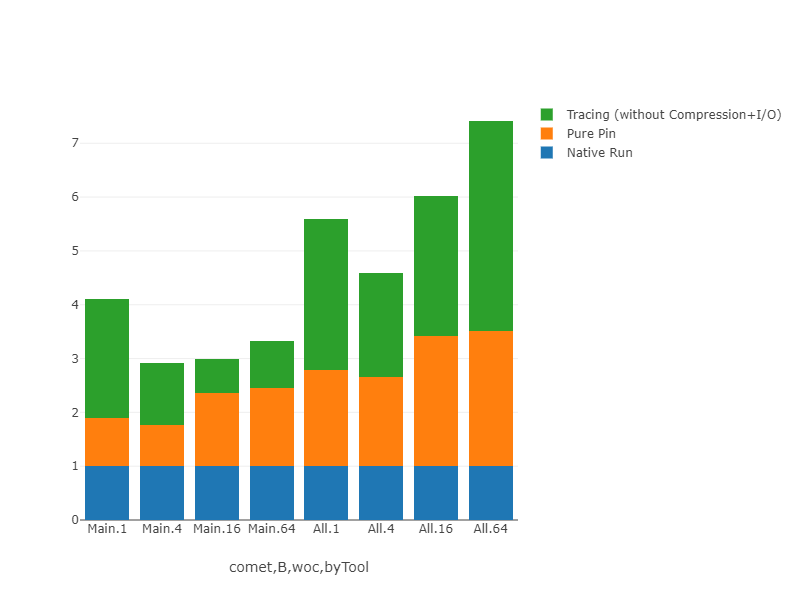
\includegraphics[width=3in,height=1.95in]{figs.comet.newMed/comet_chartDet_B_woc_byTool_p3_5.png}
\caption{\parlotnc tracing overhead breakdown - Input B}
\label{comet_chartDet_B_woc_byTool_p3_5}
\end{figure}

\begin{figure}[t]
\centering
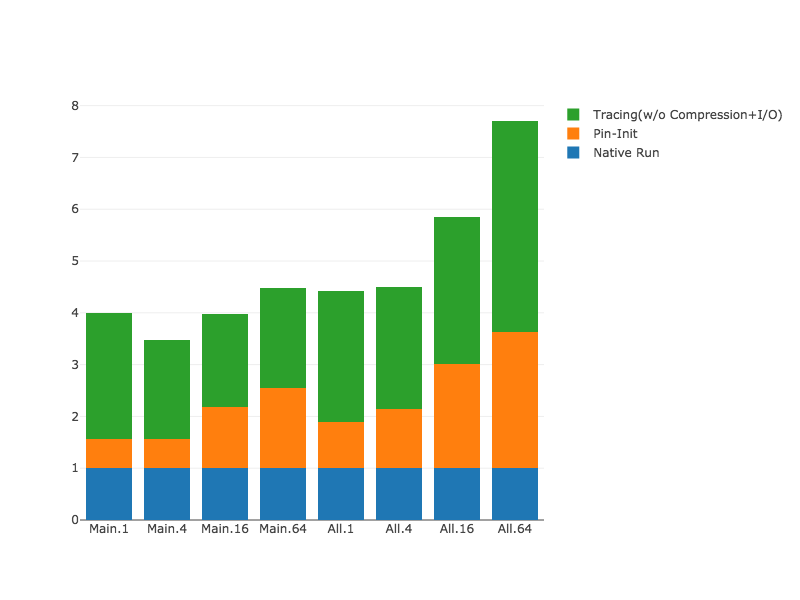
\includegraphics[width=3in,height=1.95in]{figs.comet.newMed/comet_chartDet_C_woc_byTool_p3_5.png}
\caption{ \parlotnc tracing overhead breakdown - Input C}
\label{comet_chartDet_C_woc_byTool_p3_5}
\end{figure}

In general, one 
expects the following inequality to hold:
 the overhead of \pininit should be less than that of \parlot
, which should be less than that of \parlotnc. 
%
This is not always the case because of the non-deterministic runtimes of the applications.
%
In fact, the variability across three runs of each experiment
is shown in Fig. \ref{comet_BX2_Main_16_B_p3_5}
where we present the minimum, maximum and median overheads.
%
These
overheads are for input size B and 16 nodes. 
%
This variability explains the seeming inconsistencies in  Tables
\ref{comet_wo_det_Main_all_B_p3.5} and
\ref{comet_wo_det_All_all_B_p3.5}.


On average, \pininit adds
an overhead of 3.28  and \parlota adds an overhead of 3.42. 
%
This means that \textbf{almost 96\%
of \parlota's overhead is due to \pin}. 
%
The results of \parlotm and
other inputs follow the same pattern
(as Fig. \ref{comet_chartDet_B_wc_byTool_p3_5} and \ref{comet_chartDet_C_wc_byTool_p3_5} show). 
%
The overhead that \parlot (excluding the overhead of \pininit) {\em adds}
to the applications is very small.
%
If we were to switch to a different
instrumentation tool that is not as general as \pin but more
lightweight, the overhead would potentially reduce drastically. \\


\subsection{Compression Impact} 
\label{subsec:compact}

Fig. \ref{comet_chartDet_B_woc_byTool_p3_5} and Fig. \ref{comet_chartDet_C_woc_byTool_p3_5} show the breakdown overhead by \parlotnc which illustrate the impact of compression; they also highlight the importance of incorporating compression directly in the tracing tool. 
%
On average, \parlotnc slows down the application execution almost \textbf{2x} more than \parlota. 
%
The average overhead 
across Table \ref{comet_wo_det_All_all_B_p3.5} for \parlota is \textbf{3.4}.
%
The  corresponding factor for \parlotnc is \textbf{6.6}. 
%
The numbers of \parlotm and input C  follow the same pattern. For example, \parlotnc slows down the application execution almost \textbf{1.66x} more than \parlotm.
%

Clearly, compression not only lowers the storage requirement but also the overhead. This is important as it shows that the extra computation to perform the compression is more than amortized by the reduction in the amount of data that need to be written out.
%

This result validates our approach and highlights that incremental, on-the-fly compression is likely essential to make whole-program tracing possible at low overhead.
%\begin{table*}[]
%\caption{Stat: sd 
 %Tools: pinMain , pinAll , callgrind ,  
 %Inputs: B ,  
 %Nodes: 1 , 4 , 16 ,  
 %Desc: Primary}
 \caption{This table contains Slowdowns of ParLOT and Callgrind (slowdowns are relative to pure run). The input size is \textbf{B}.  NAS benchmark input sizes are as follows : $size(A) < size(B) < size (C) < size(D) $. In later tables and charts I show that ParLOT has better performance on larger inputs (like C and D). I was not able to run Callgrind with input size of C and D since it was time consuming, crashing and wasting SUs. Also I only included the results for up to 16 nodes (256 cores) in this table. Almost all of the experiments with Callgrind on 64 nodes (1024 cores) crashed [I documented all sort of crashing reasons of Callgrind on 1024 cores]. ParLOT results of 64 nodes will appear in later tables. I grouped the results of experiments with similar input sizes and nodes (group of 3 rows). Each row is in this format \textbf{Tool.Input.Nodes}. Last column of the table (GM) is GeoMean of all values in that row. By comparing the values of GM row, we can see that ParLOT(both main and all) has better performance comparing to Callgrind. However, it seems that Callgrind scales better (more about this in next table). ( Fig \ref{chartAvg_sd_B_p3_5})}
 \label{sd_pMpAcg_B_int_p3.5}
\begin{center}
\begin{tabular}{|l|rrrrrrrr|r|}
\hline
                &    bt &    cg &    ep &    ft &    is &    lu &    mg &    sp &    GM \\
\hline
 pinMain.B.1    &  1.60 &  1.81 &  3.93 &  1.53 &  3.05 &  1.21 &  3.61 &  1.53 &  2.08 \\
 pinAll.B.1     &  2.01 &  3.03 &  4.63 &  2.43 &  6.86 &  1.66 &  9.10 &  1.56 &  3.20 \\
 callgrind.B.1  & 12.47 & 19.56 & 17.07 &  9.67 &  7.82 & 11.32 & 15.66 & 10.50 & 12.47 \\
 \hline
 pinMain.B.4    &  1.67 &  3.78 &  2.43 &  2.91 &  4.04 &  2.83 &  3.54 &  2.93 &  2.92 \\
 pinAll.B.4     &  3.95 &  8.96 &  3.52 &  7.67 & 10.25 &  5.83 &  6.18 &  3.70 &  5.81 \\
 callgrind.B.4  &  7.83 & 12.64 &  6.07 &  6.18 &  2.89 & 20.14 &  4.70 & 12.04 &  7.69 \\
 \hline
 pinMain.B.16   &  3.68 &  7.80 &  9.90 &  5.45 &  4.41 &  3.81 &  3.51 &  2.41 &  4.65 \\
 pinAll.B.16    &  6.55 & 12.53 &  6.47 & 10.40 &  5.45 &  4.01 &  6.35 &  4.73 &  6.61 \\
 callgrind.B.16 & 10.95 & 28.44 &  9.23 &  7.90 &  4.04 &  8.89 &  8.55 &  6.16 &  9.00 \\
\hline
\end{tabular}
\end{center}
\end{table*}

\begin{table*}[]
\caption{Server: \textbf{Comet} - 
 Stat: \textbf{Detail Slowdown} -
 Tools: pinMain , pinAll , callgrind - 
 Inputs: B - 
 Nodes: 1 , 4 , 16 , 64 - 
 Desc: Primary - Similar to table \ref{sd_pMpAcg_B_int_p3.5} but numbers are from Comet}
\label{comet_sd_pMpAcg_B_int_p3.5}\begin{center}
\begin{tabular}{|l|rrrrrrrr|r|}
\hline
                &   bt &   cg &   ep &    ft &   is &   lu &   mg &   sp &   GM \\
\hline
 pinMain.B.1    & 1.55 & 1.82 & 2.68 &  2.11 & 2.48 & 1.31 & 2.57 & 1.33 & 1.91 \\
 pinAll.B.1     & 1.85 & 2.73 & 4.21 &  2.85 & 4.52 & 1.74 & 5.57 & 1.73 & 2.87 \\
 callgrind.B.1  & 8.68 & 6.07 & 9.31 & 10.33 & 2.64 & 7.61 & 3.39 & 6.62 & 6.24 \\
  \hline
 pinMain.B.4    & 1.76 & 1.85 & 1.92 &  1.74 & 1.79 & 1.77 & 1.83 & 1.76 & 1.80 \\
 pinAll.B.4     & 2.63 & 3.11 & 3.41 &  2.86 & 3.03 & 2.82 & 3.10 & 2.76 & 2.96 \\
 callgrind.B.4  & 6.13 & 3.63 & 2.95 &  3.50 & 1.46 & 5.41 & 1.43 & 5.98 & 3.34 \\
  \hline
 pinMain.B.16   & 2.19 & 2.62 & 2.39 &  1.93 & 1.82 & 2.80 & 2.43 & 2.23 & 2.28 \\
 pinAll.B.16    & 3.73 & 4.20 & 4.36 &  2.96 & 2.84 & 4.30 & 4.49 & 3.71 & 3.77 \\
 callgrind.B.16 & 4.31 & 3.26 & 2.39 &  2.20 & 1.73 & 4.70 & 1.92 & 4.65 & 2.93 \\
 \hline
 pinMain.B.64   & 2.45 & 2.72 & 2.45 &  1.99 & 4.34 & 4.56 & 2.31 & 2.46 & 2.79 \\
 pinAll.B.64    & 4.22 & 4.19 & 4.55 &  3.13 & 5.46 & 4.73 & 4.17 & 4.23 & 4.29 \\
 callgrind.B.64 & 2.85 & 2.71 & 1.86 &  2.16 & 4.13 & 4.10 & 1.87 & 3.54 & 2.77 \\
\hline
\end{tabular}
\end{center}
\end{table*}



\begin{table*}[]
%\caption{Stat: sd 
 %Tools: pinMain , pinAll , callgrind ,  
 %Inputs: B ,  
 %Nodes: 1 , 4 , 16 ,  
 %Desc: Primary} 

\caption{The values in this table is identical to table \ref{sd_pMpAcg_B_int_p3.5} but grouped differently to show the scalability of each tool. The slowdown of Callgrind drops drastically with increasing cores from 16 to 64. For ParLOT (for both main and all), slowdowns are higher for larger number of cores. However, the average GeoMean of all slowdowns (numbers in bold) show that ParLOT has better overall performance. The \textbf{AVG} rows contain the average of its above 3 values.( Fig \ref{chartAvg_sd_B_p3_5})}

\label{sd_pMpAcg_B_itn_p3.5}
\begin{center}
\begin{tabular}{|l|rrrrrrrr|r|}
\hline
                &    bt &    cg &    ep &    ft &    is &    lu &    mg &    sp &    GM \\
\hline
 pinMain.B.1    &  1.60 &  1.81 &  3.93 &  1.53 &  3.05 &  1.21 &  3.61 &  1.53 &  2.08 \\
 pinMain.B.4    &  1.67 &  3.78 &  2.43 &  2.91 &  4.04 &  2.83 &  3.54 &  2.93 &  2.92 \\
 pinMain.B.16   &  3.68 &  7.80 &  9.90 &  5.45 &  4.41 &  3.81 &  3.51 &  2.41 &  4.65 \\
 \hline
 AVG            &  2.32 &  4.46 &  5.42 &  3.30 &  3.83 &  2.62 &  3.55 &  2.29 &  \textbf{3.22} \\
 \hline
 pinAll.B.1     &  2.01 &  3.03 &  4.63 &  2.43 &  6.86 &  1.66 &  9.10 &  1.56 &  3.20 \\
 pinAll.B.4     &  3.95 &  8.96 &  3.52 &  7.67 & 10.25 &  5.83 &  6.18 &  3.70 &  5.81 \\
 pinAll.B.16    &  6.55 & 12.53 &  6.47 & 10.40 &  5.45 &  4.01 &  6.35 &  4.73 &  6.61 \\
 \hline
 AVG            &  4.17 &  8.17 &  4.87 &  6.83 &  7.52 &  3.83 &  7.21 &  3.33 &  \textbf{5.21} \\
 \hline
 callgrind.B.1  & 12.47 & 19.56 & 17.07 &  9.67 &  7.82 & 11.32 & 15.66 & 10.50 & 12.47 \\
 callgrind.B.4  &  7.83 & 12.64 &  6.07 &  6.18 &  2.89 & 20.14 &  4.70 & 12.04 &  7.69 \\
 callgrind.B.16 & 10.95 & 28.44 &  9.23 &  7.90 &  4.04 &  8.89 &  8.55 &  6.16 &  9.00 \\
 \hline
 AVG            & 10.42 & 20.21 & 10.79 &  7.92 &  4.92 & 13.45 &  9.64 &  9.57 &  \textbf{9.72} \\
 
\hline
\end{tabular}
\end{center}
\end{table*}



\begin{figure*}[!t]
\centering
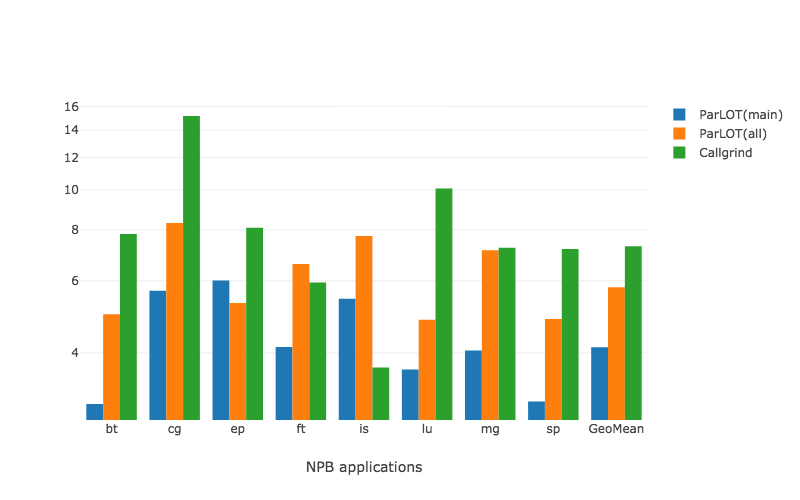
\includegraphics[width=5in]{figs.psc/chartAvg_sd_B_p3_5.png}
\caption{ Slowdown of ParLOT(main,all) and Callgrind. Each bar is the average slowdown of each tool on each application for 1, 4 and 16 nodes (16, 64 and 256 cores). Last group of bars is GeoMean (from bold numbers in table \ref{sd_pMpAcg_B_itn_p3.5}). 
}
\label{chartAvg_sd_B_p3_5}
\end{figure*}

\begin{table*}[]
\caption{Server: \textbf{Comet} - 
 Stat: \textbf{Detail Slowdown} -
 Tools: pinMain , pinAll , callgrind -  
 Inputs: B -
 Nodes: 1 , 4 , 16 , 64 -
 Desc: Primary  - Similar to table \ref{sd_pMpAcg_B_itn_p3.5} but numbers are from Comet}
\label{comet_sd_pMpAcg_B_itn_p3.5}
\begin{center}
\begin{tabular}{|l|rrrrrrrr|r|}
\hline
                &   bt &   cg &   ep &    ft &   is &   lu &   mg &   sp &   GM \\
\hline
 pinMain.B.1    & 1.55 & 1.82 & 2.68 &  2.11 & 2.48 & 1.31 & 2.57 & 1.33 & 1.91 \\
 pinMain.B.4    & 1.76 & 1.85 & 1.92 &  1.74 & 1.79 & 1.77 & 1.83 & 1.76 & 1.80 \\
 pinMain.B.16   & 2.19 & 2.62 & 2.39 &  1.93 & 1.82 & 2.80 & 2.43 & 2.23 & 2.28 \\
 pinMain.B.64   & 2.45 & 2.72 & 2.45 &  1.99 & 4.34 & 4.56 & 2.31 & 2.46 & 2.79 \\
 \hline
 AVG            & 1.99 & 2.25 & 2.36 &  1.94 & 2.61 & 2.61 & 2.29 & 1.95 & \textbf{2.20} \\
 \hline
 pinAll.B.1     & 1.85 & 2.73 & 4.21 &  2.85 & 4.52 & 1.74 & 5.57 & 1.73 & 2.87 \\
 pinAll.B.4     & 2.63 & 3.11 & 3.41 &  2.86 & 3.03 & 2.82 & 3.10 & 2.76 & 2.96 \\
 pinAll.B.16    & 3.73 & 4.20 & 4.36 &  2.96 & 2.84 & 4.30 & 4.49 & 3.71 & 3.77 \\
 pinAll.B.64    & 4.22 & 4.19 & 4.55 &  3.13 & 5.46 & 4.73 & 4.17 & 4.23 & 4.29 \\
 \hline
 AVG            & 3.11 & 3.56 & 4.13 &  2.95 & 3.96 & 3.40 & 4.33 & 3.11 & \textbf{3.47} \\
 \hline
 callgrind.B.1  & 8.68 & 6.07 & 9.31 & 10.33 & 2.64 & 7.61 & 3.39 & 6.62 & 6.24 \\
 callgrind.B.4  & 6.13 & 3.63 & 2.95 &  3.50 & 1.46 & 5.41 & 1.43 & 5.98 & 3.34 \\
 callgrind.B.16 & 4.31 & 3.26 & 2.39 &  2.20 & 1.73 & 4.70 & 1.92 & 4.65 & 2.93 \\
 callgrind.B.64 & 2.85 & 2.71 & 1.86 &  2.16 & 4.13 & 4.10 & 1.87 & 3.54 & 2.77 \\
 \hline
 AVG            & 5.49 & 3.92 & 4.13 &  4.55 & 2.49 & 5.46 & 2.15 & 5.20 & \textbf{3.82} \\
\hline
\end{tabular}
\end{center}
\end{table*}




\begin{table*}[]
%\caption{Stat: bw 
% Tools: pinMain , pinAll , callgrind ,  
% Inputs: B ,  
% Nodes: 1 , 4 , 16 ,  
% Desc: Primary}


\caption{This table is showing the required bandwidth for each application (KiloBytes per core per second). $ReqBW_x = TraceSize_x (KB) / (\# of cores)_x / Runtime_x (S)$
Because of the crashing problems of Callgrind on \textit{C} input and 64 nodes, I only include \textit{B} input and 1, 4, and 16 nodes results. Clearly ParLOT(main) is beating Callgrind while they both generate the same information (I still believe ParLOT(main) generated traces are more informative and rich). ParLOT(all) bandwidth is the highest but with capturing all of the function calls within a single execution, there is no surprise. Another interesting fact from this table is, for ParLOT(main), bandwidth drops from \textbf{0.62} for 16 cores to \textbf{0.27} for 256 cores (good scalability). It is the opposite for Callgrind where the required bandwidth jumps from \textbf{3.28} (KB/s) for 16 cores to \textbf{33.06} (KB/S) for 256 cores. I also have the results of required bandwidth of ParLOT for 64 nodes(1024 cores) and Input C but I did not include them here because I did not have them for Callgrind (explained above).  Fig \ref{chartAvg_bw_B_p3_5} visualize these numbers (Average values)}
\label{bw_pMpAcg_B_itn_p3.5}
\begin{center}
\begin{tabular}{|l|rrrrrrrr|r|}
\hline
                &    bt &    cg &    ep &    ft &    is &    lu &    mg &    sp &    GM \\
\hline
 pinMain.B.1    &  2.54 & 22.73 &  0.99 &  0.33 &  0.46 &  0.10 &  0.43 &  0.06 &  0.62 \\
 pinMain.B.4    &  3.20 & 18.31 &  0.52 &  0.20 &  0.12 &  0.11 &  0.23 &  0.10 &  0.46 \\
 pinMain.B.16   &  2.20 &  9.66 &  0.09 &  0.14 &  0.06 &  0.08 &  0.19 &  0.13 &  0.27 \\
 \hline
 AVG            &  2.65 & 16.90 &  0.53 &  0.22 &  0.21 &  0.10 &  0.28 &  0.10 &  \textbf{0.45} \\
 \hline
 pinAll.B.1     & 20.80 & 39.89 & 14.75 & 21.05 & 31.00 & 19.55 & 34.37 & 12.37 & 22.53 \\
 pinAll.B.4     & 21.85 & 33.10 & 22.15 & 17.05 & 16.19 & 35.84 & 34.53 & 35.99 & 25.81 \\
 pinAll.B.16    & 25.31 & 29.33 & 23.31 & 20.07 & 23.78 & 56.58 & 29.09 & 42.96 & 29.57 \\
 \hline
 AVG            & 22.65 & 34.11 & 20.07 & 19.39 & 23.66 & 37.32 & 32.66 & 30.44 & \textbf{25.97} \\
 \hline
 callgrind.B.1  &  0.90 &  2.40 &  2.53 &  4.02 & 24.33 &  1.39 & 14.64 &  1.22 &  3.28 \\
 callgrind.B.4  &  4.27 &  9.11 & 12.02 & 16.78 & 59.03 &  2.97 & 35.78 &  5.20 & 11.25 \\
 callgrind.B.16 & 17.48 & 12.87 & 46.08 & 51.94 & 87.05 & 19.13 & 48.00 & 33.18 & 33.06 \\
 \hline
 AVG            &  7.55 &  8.13 & 20.21 & 24.25 & 56.80 &  7.83 & 32.81 & 13.20 & \textbf{15.86} \\
\hline
\end{tabular}
\end{center}
\end{table*}


\begin{figure*}[!t]
\centering
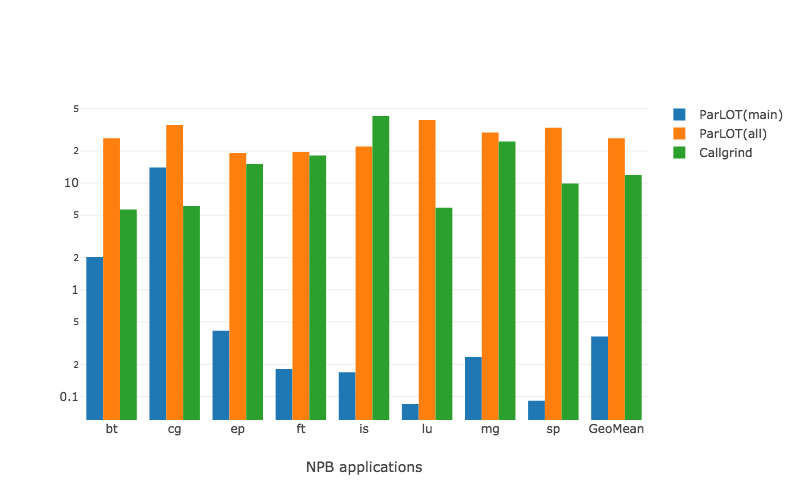
\includegraphics[width=5in]{figs.psc/chartAvg_bw_B_p3_5.png}
\caption{ Required Bandwidth (KB) per core per second for ParLOT and Callgrind.  
(Input: B)}
\label{chartAvg_bw_B_p3_5}
\end{figure*}

\begin{table*}[]
\caption{Server: \textbf{Comet} -
 Stat: \textbf{Bandwidth} -
 Tools: pinMain , pinAll , callgrind - 
 Inputs: B -
 Nodes: 1 , 4 , 16 , 64 -
 Desc: Primary}
\label{comet_bw_pMpAcg_B_itn_p3.5}\begin{center}
\begin{tabular}{|l|rrrrrrrr|r|}
\hline
                &    bt &     cg &    ep &    ft &    is &     lu &    mg &    sp &    GM \\
\hline
 pinMain.B.1    &  4.72 &  21.86 &  3.83 &  1.52 &  0.79 &   2.39 &  5.62 &  5.36 &  3.69 \\
 pinMain.B.4    & 14.28 &  41.08 &  1.89 &  3.48 &  2.24 &  21.48 &  6.45 & 15.85 &  8.12 \\
 pinMain.B.16   & 14.31 &  46.59 &  1.45 &  4.86 &  3.40 &  31.79 &  6.53 & 18.55 &  9.41 \\
 pinMain.B.64   & 18.56 &  43.59 &  1.25 &  4.56 &  4.49 &  27.07 &  5.63 & 29.62 &  9.92 \\
 \hline
 AVG            & 12.97 &  38.28 &  2.10 &  3.60 &  2.73 &  20.68 &  6.06 & 17.35 &  7.79 \\
 \hline
 pinAll.B.1     & 48.71 &  89.39 & 47.23 & 45.63 & 59.98 &  53.62 & 60.81 & 54.33 & 56.21 \\
 pinAll.B.4     & 61.84 & 101.23 & 45.21 & 55.12 & 53.20 &  71.09 & 54.85 & 73.62 & 62.68 \\
 pinAll.B.16    & 73.95 & 116.87 & 47.37 & 48.88 & 47.79 & 100.91 & 55.80 & 84.61 & 67.97 \\
 pinAll.B.64    & 81.80 & 110.15 & 44.16 & 47.98 & 37.84 & 100.26 & 52.67 & 99.90 & 66.47 \\
 \hline
 AVG            & 66.58 & 104.41 & 45.99 & 49.40 & 49.70 &  81.47 & 56.03 & 78.12 & 63.33 \\
 \hline
 callgrind.B.1  &  1.57 &   7.69 &  7.39 &  4.56 & 39.49 &   2.61 & 34.41 &  2.71 &  6.67 \\
 callgrind.B.4  &  6.51 &  16.01 & 22.10 & 15.65 & 45.46 &   8.63 & 45.47 &  7.78 & 16.31 \\
 callgrind.B.16 & 17.20 &  24.62 & 37.42 & 23.84 & 29.87 &  16.23 & 51.49 & 15.81 & 24.93 \\
 callgrind.B.64 & 26.82 &  27.65 & 45.93 & 25.14 & 11.04 &  17.75 & 45.27 & 20.20 & 25.02 \\
 \hline
 AVG            & 13.03 &  18.99 & 28.21 & 17.30 & 31.47 &  11.30 & 44.16 & 11.62 & 18.23 \\
\hline
\end{tabular}
\end{center}
\end{table*}




\begin{table*}[]
%\caption{Stat: cr 
% Tools: pinMain , pinAll ,  
% Inputs: C , B ,  
% Nodes: 1 , 4 , 16 , 64 ,  
% Desc: Primary}
\caption{COMPRESSION RATIOS FOR B AND C INPUTS AND 1, 4, 16 AND 64 NODES.}
\label{cr_pMpA_BC_itn_p3.5}
\begin{center}
\begin{tabular}{|l|rrrrrrrr|r|}
\hline
              &       bt &      cg &       ep &       ft &       is &       lu &      mg &       sp &      GM \\
\hline
 pinMain.C.1  & 14051.90 &   85.18 & 12104.15 & 31406.62 & 36422.85 & 20423.90 & 1169.56 & 22561.69 & 7393.79 \\
 pinMain.C.4  &  8249.54 &   85.36 & 12067.24 & 24222.90 & 33655.89 & 11191.63 &  650.18 & 10441.99 & 5189.93 \\
 pinMain.C.16 &  1985.31 &   85.55 & 11921.80 & 11426.88 & 25812.61 &  7353.92 &  353.38 &  4810.38 & 3048.85 \\
 pinMain.C.64 &   709.30 &   85.74 & 11374.25 &  6738.89 & 13360.80 &  6916.77 &  250.95 &  4624.28 & 2174.51 \\
 \hline
 AVG          &  6249.01 &   85.46 & 11866.86 & 18448.82 & 27313.04 & 11471.56 &  606.02 & 10609.58 & 4451.77 \\
 \hline
 pinAll.C.1   &  2579.37 &   89.08 & 21213.12 &  6818.31 &  7698.78 &   135.16 &   89.48 &   272.48 &  978.90 \\
 pinAll.C.4   &  1441.93 &  301.17 & 13242.06 &  1412.63 &  1122.81 &   709.17 &  857.56 &   773.11 & 1199.60 \\
 pinAll.C.16  &  1954.84 &  413.29 &  6721.88 &  1531.17 &  1793.81 &   430.15 & 1317.55 &   820.22 & 1273.86 \\
 pinAll.C.64  &  1195.58 &  891.83 &  5537.37 &  3191.36 &  2461.46 &   676.34 & 2412.46 &   967.72 & 1710.36 \\
 \hline
 AVG          &  1792.93 &  423.84 & 11678.61 &  3238.37 &  3269.22 &   487.71 & 1169.26 &   708.38 & 1290.68 \\
 \hline
 pinMain.B.1  &  5403.04 &   74.95 & 12067.06 & 12704.90 & 33655.87 &  8750.65 &  541.98 & 10426.05 & 4234.22 \\
 pinMain.B.4  &  2129.01 &   75.33 & 11922.18 & 10745.40 & 25812.57 &  5128.06 &  364.22 &  4042.15 & 2820.40 \\
 pinMain.B.16 &   729.64 &   75.70 & 11374.86 &  3508.41 & 13360.75 &  4371.76 &  205.67 &  3265.36 & 1746.25 \\
 pinMain.B.64 &  3551.97 &   76.08 &  9608.18 &  2790.59 &  4563.29 &  4031.59 &  164.19 &  4030.09 & 1750.60 \\
 \hline
 AVG          &  2953.41 &   75.52 & 11243.07 &  7437.32 & 19348.12 &  5570.52 &  319.02 &  5440.91 & 2637.87 \\
 \hline
 pinAll.B.1   &   750.27 &   68.40 & 16927.14 &  2584.15 &  2304.36 &   101.34 &   69.80 &   119.94 &  507.33 \\
 pinAll.B.4   &  1693.37 &  649.30 &  6797.11 &  2165.42 &  2402.91 &   727.52 &  836.96 &   672.73 & 1413.43 \\
 pinAll.B.16  &  1265.26 & 1138.20 &  4140.31 &  1794.78 &  1993.44 &   620.41 & 1477.61 &   883.86 & 1427.94 \\
 pinAll.B.64  &  1294.03 & 1218.33 &  5187.85 &  3086.80 &  3266.69 &  1044.65 & 2520.99 &  1167.23 & 1997.57 \\
 \hline
 AVG          &  1250.73 &  768.56 &  8263.10 &  2407.79 &  2491.85 &   623.48 & 1226.34 &   710.94 & 1336.57 \\

\hline
\end{tabular}
\end{center}
\end{table*}

\begin{table*}[]
\caption{Server: \textbf{Comet} - \textbf{COMPRESSION RATIOS} FOR B INPUTS AND 1, 4, 16 AND 64 NODES - C input experiments are cooking}
\label{comet_cr_pMpA_B_itn_p3.5}\begin{center}
\begin{tabular}{|l|rrrrrrrr|r|}
\hline
              &      bt &     cg &       ep &       ft &      is &     lu &     mg &     sp &      GM \\
\hline
 pinMain.B.1  & 3035.93 &  94.35 & 12456.18 & 12173.49 & 9718.38 & 167.72 &  99.08 & 878.27 & 1255.17 \\
 pinMain.B.4  &  586.64 &  82.48 & 10368.41 &  1737.09 &  909.20 & 140.29 & 254.95 & 338.16 &  559.36 \\
 pinMain.B.16 &  346.66 & 113.28 &  8563.85 &  1077.35 & 1200.57 & 178.98 & 387.63 & 123.02 &  496.83 \\
 pinMain.B.64 &  252.24 & 147.78 &  7611.04 &  1122.62 & 1907.95 & 366.80 & 437.31 & 152.91 &  591.11 \\
 \hline
 AVG          & 1055.37 & 109.47 &  9749.87 &  4027.64 & 3434.03 & 213.45 & 294.74 & 373.09 &  725.62 \\
 \hline
 pinAll.B.1   &  514.51 & 137.41 &  3335.77 &  1226.74 &  543.18 & 314.63 & 260.87 & 303.88 &  500.21 \\
 pinAll.B.4   &  315.71 & 137.21 &  1266.92 &   436.15 &  316.16 & 287.25 & 329.57 & 199.66 &  330.70 \\
 pinAll.B.16  &  226.86 & 181.58 &  1246.66 &  1026.53 &  927.09 & 299.30 & 469.29 & 171.52 &  430.39 \\
 pinAll.B.64  &  329.23 & 247.30 &  1394.07 &  1043.94 & 1984.62 & 410.32 & 548.47 & 307.16 &  597.55 \\
 \hline
 AVG          &  346.58 & 175.88 &  1810.86 &   933.34 &  942.76 & 327.88 & 402.05 & 245.56 &  464.71 \\
\hline
\end{tabular}
\end{center}
\end{table*}



\begin{table*}[]
%\caption{Stat: sd 
% Tools:  
% Inputs: B ,  
% Nodes: 1 , 4 , 16 , 64 ,  
% Desc: Detail Report}

\caption{Server: \textbf{PSC} - Tables \ref{det_Main_all_B_p3.5}, \ref{comet_det_Main_all_B_p3.5}, \ref{ls5_det_Main_all_B_p3.5}, \ref{det_All_all_B_p3.5}, \ref{comet_det_All_all_B_p3.5} and \ref{ls5_det_All_all_B_p3.5}  are showing the detail slowdowns added to the code by each phase of ParLOT(main and all) for input size \textit{B} on \textbf{PSC}, \textbf{Comet} and \textbf{Lonestar5}. I put my observations of all four tables over here. \textbf{npin} is just the slowdown caused by initializing Pin's routines on top of the target application without doing anything else (no instrumentation, tracing, compression and I/O.  \textbf{dpin} is almost identical to ParLOT except it stores the generated compressed traces to "/dev/null". The purpose of \textit{dpin} is to see how much of the overall overhead is because of I/O and data-related slowdowns. In \textbf{wpin}, and all collected data would be stored as is to the disk. The results of this tools shows how much efficiency our compression approach adds to ParLOT. Last row of tables shows geometric mean of each of its above values showing how much each phase of ParLOT slows down the native execution. In general, we all expect that the slowdowns of $npin < dpin < ParLOT < wpin $. But majority of numbers are not like that. I double checked the results of CHPC and Stampede and the patterns are kind of identical.  In most of the table entries (in particular for smaller number of cores), the differences between the average slowdown of \textit{dpin} and \textit{ParLOT} is very insignificant which shows that ParLOT is not an I/O-bounded tool. Figures \ref{chartDet_B_wc_byTool_p3_5} and \ref{chartDet_B_woc_byTool_p3_5} visualize numbers from these tables.} 
\label{det_Main_all_B_p3.5}

\begin{center}
\scalebox{0.95}{
\begin{tabular}{|c|c|rrrr|rrrr|rrrr|rrrr|} 
\hline 
\multicolumn{1}{|l|}{\multirow{2}{*}{\textbf{Input: B}}} & \multicolumn{1}{r|}{Nodes :}    & \multicolumn{4}{c|}{1}  & \multicolumn{4}{c|}{4} & \multicolumn{4}{c|}{16}  & \multicolumn{4}{c|}{64} \\ \cline{2-18} 
\multicolumn{1}{|l|}{} & \multicolumn{1}{r|}{Detail Tools:} & \multicolumn{1}{c}{npin} & \multicolumn{1}{c}{dpin} & \multicolumn{1}{c}{ParLOT} & \multicolumn{1}{c|}{wpin} & \multicolumn{1}{c}{npin} & \multicolumn{1}{c}{dpin} & \multicolumn{1}{c}{ParLOT} & \multicolumn{1}{c|}{wpin} & \multicolumn{1}{c}{npin} & \multicolumn{1}{c}{dpin} & \multicolumn{1}{c}{ParLOT} & \multicolumn{1}{c|}{wpin} & \multicolumn{1}{c}{npin} & \multicolumn{1}{c}{dpin} & \multicolumn{1}{c}{ParLOT} & \multicolumn{1}{c|}{wpin} \\
\hline
\multirow{9}{*}{Main} &  bt  &  1.49  &  1.52  &  1.60  &  11.63  &  1.17  &  1.58  &  1.67  &  8.53  &  1.86  &  2.99  &  3.68  &   8.81  &  4.22  &  4.51  &   5.07  &  13.64 \\
 &  cg  &  1.78  & \cellcolor{blue!25} 1.76  &  1.81  &   3.19  &  2.64  &  5.02  & \cellcolor{blue!25} 3.78  &  6.76  &  4.86  &  6.27  &  7.80  &  12.38  &  3.92  &  8.43  &   9.31  &  12.96 \\
 &  ep  &  3.82  & \cellcolor{blue!25} 3.37  &  3.93  &  22.47  &  1.84  &  2.26  &  2.43  &  7.94  &  4.97  &  5.02  &  9.90  & \cellcolor{blue!25}  9.09  &  3.27  &  7.22  &   7.78  &   7.67 \\
 &  ft  &  1.60  & \cellcolor{blue!25} 1.51  &  1.53  &   3.23  &  2.43  &  4.36  & \cellcolor{blue!25} 2.91  &  4.31  &  3.52  &  5.90  & \cellcolor{blue!25} 5.45  &   5.87  &  3.24  &  6.87  & \cellcolor{blue!25}  6.67  &   6.69 \\
 &  is  &  3.61  & \cellcolor{blue!25} 3.55  & \cellcolor{blue!25} 3.05  &  14.60  &  3.20  &  3.68  &  4.04  &  5.88  &  3.85  &  4.82  & \cellcolor{blue!25} 4.41  &   4.67  &  4.80  &  9.99  &  10.19  &  10.46 \\
 &  lu  &  1.39  & \cellcolor{blue!25} 1.20  &  1.21  &   1.58  &  1.85  &  2.07  &  2.83  &  3.52  &  1.64  &  3.00  &  3.81  &   5.53  &  3.17  &  6.77  & \cellcolor{blue!25}  6.73  &  13.70 \\
 &  mg  &  3.91  & \cellcolor{blue!25} 3.51  &  3.61  &   3.84  &  3.19  &  3.34  &  3.54  &  3.96  &  2.95  &  3.36  &  3.51  &   3.82  &  3.70  &  5.57  & \cellcolor{blue!25}  5.56  &   5.70 \\
 &  sp  &  1.25  &  1.43  &  1.53  &   1.65  &  2.13  &  4.38  & \cellcolor{blue!25} 2.93  &  3.63  &  2.98  &  3.48  & \cellcolor{blue!25} 2.41  &   3.86  &  4.28  &  5.78  & \cellcolor{blue!25}  5.30  &   8.56 \\ \cline{2-18}
 &  GM  &  2.11  & \cellcolor{blue!25} 2.03  &  2.08  &   5.00  &  2.20  &  3.11  & \cellcolor{blue!25} 2.92  &  5.26  &  3.11  &  4.18  &  4.65  &   6.21  &  3.79  &  6.71  &   6.87  &   9.45 \\
\hline 
\end{tabular} }

\end{center}
\end{table*}









\begin{table*}[]
\caption{Server: \textbf{Comet} - 
 Stat: \textbf{Detail Slowdown} -
 Inputs: B -
 Nodes: 1 , 4 , 16 , 64 -
 Desc: Detail Report}
\begin{center}
\label{comet_det_Main_all_B_p3.5}
\scalebox{0.95}{
\begin{tabular}{|c|c|rrrr|rrrr|rrrr|rrrr|} 
\hline 
\multicolumn{1}{|l|}{\multirow{2}{*}{\textbf{Input: B}}} & \multicolumn{1}{r|}{Nodes :}    & \multicolumn{4}{c|}{1}  & \multicolumn{4}{c|}{4} & \multicolumn{4}{c|}{16}  & \multicolumn{4}{c|}{64} \\ \cline{2-18} 
\multicolumn{1}{|l|}{} & \multicolumn{1}{r|}{Detail Tools:} & \multicolumn{1}{c}{npin} & \multicolumn{1}{c}{dpin} & \multicolumn{1}{c}{ParLOT} & \multicolumn{1}{c|}{wpin} & \multicolumn{1}{c}{npin} & \multicolumn{1}{c}{dpin} & \multicolumn{1}{c}{ParLOT} & \multicolumn{1}{c|}{wpin} & \multicolumn{1}{c}{npin} & \multicolumn{1}{c}{dpin} & \multicolumn{1}{c}{ParLOT} & \multicolumn{1}{c|}{wpin} & \multicolumn{1}{c}{npin} & \multicolumn{1}{c}{dpin} & \multicolumn{1}{c}{ParLOT} & \multicolumn{1}{c|}{wpin} \\
\hline
\multirow{9}{*}{Main} &  bt  &  1.50  &  1.56  & \cellcolor{blue!25} 1.55  &   5.66  &  1.74  &  1.79  & \cellcolor{blue!25} 1.76  &  5.19  &  2.21  & \cellcolor{blue!25} 2.13  &  2.19  &  11.49  &  2.29  &  2.48  & \cellcolor{blue!25} 2.45  &  17.89 \\
 &  cg  &  1.75  &  1.87  & \cellcolor{blue!25} 1.82  &   2.39  &  1.95  & \cellcolor{blue!25} 1.84  &  1.85  &  2.64  &  2.72  & \cellcolor{blue!25} 2.52  &  2.62  &  12.39  &  2.67  & \cellcolor{blue!25} 2.35  &  2.72  &  22.61 \\
 &  ep  &  2.97  & \cellcolor{blue!25} 2.74  & \cellcolor{blue!25} 2.68  &  21.44  &  2.07  & \cellcolor{blue!25} 1.90  &  1.92  &  5.82  &  2.58  & \cellcolor{blue!25} 2.34  &  2.39  &   4.22  &  2.81  & \cellcolor{blue!25} 2.52  & \cellcolor{blue!25} 2.45  &   3.28 \\
 &  ft  &  1.87  &  2.10  &  2.11  &   6.29  &  1.76  &  1.76  & \cellcolor{blue!25} 1.74  &  2.85  &  2.13  & \cellcolor{blue!25} 1.88  &  1.93  &   2.59  &  2.23  & \cellcolor{blue!25} 1.89  &  1.99  &   2.34 \\
 &  is  &  2.51  &  2.54  & \cellcolor{blue!25} 2.48  &   4.87  &  1.80  & \cellcolor{blue!25} 1.78  &  1.79  &  2.08  &  2.11  & \cellcolor{blue!25} 1.76  &  1.82  &   2.24  &  4.76  & \cellcolor{blue!25} 4.31  &  4.34  &   6.29 \\
 &  lu  &  1.32  & \cellcolor{blue!25} 1.31  &  1.31  &   1.44  &  1.77  &  1.78  & \cellcolor{blue!25} 1.77  &  2.27  &  2.74  & \cellcolor{blue!25} 2.66  &  2.80  &   4.06  &  3.05  & \cellcolor{blue!25} 2.81  &  4.56  &   7.94 \\
 &  mg  &  2.64  & \cellcolor{blue!25} 2.62  & \cellcolor{blue!25} 2.57  &   2.80  &  1.75  & \cellcolor{blue!25} 1.69  &  1.83  &  1.79  &  2.64  & \cellcolor{blue!25} 2.36  &  2.43  &   3.23  &  2.37  & \cellcolor{blue!25} 2.15  &  2.31  &   2.81 \\
 &  sp  &  1.35  &  1.35  & \cellcolor{blue!25} 1.33  &   2.47  &  1.74  &  1.76  &  1.76  &  3.72  &  2.15  & \cellcolor{blue!25} 2.03  &  2.23  &   2.94  &  2.29  & \cellcolor{blue!25} 2.18  &  2.46  &   6.84 \\ \cline{2-18}
 &  GM  &  1.90  &  1.94  & \cellcolor{blue!25} 1.91  &   4.15  &  1.82  & \cellcolor{blue!25} 1.79  &  1.80  &  3.03  &  2.40  & \cellcolor{blue!25} 2.19  &  2.28  &   4.38  &  2.72  & \cellcolor{blue!25} 2.51  &  2.79  &   6.45 \\
\hline 
\end{tabular} }

\end{center}
\end{table*}



\begin{table*}[]
\caption{Input: B ,  All}
\label{det_All_all_B_p3.5}
\begin{center}
\scalebox{0.95}{
\begin{tabular}{|c|c|rrrr|rrrr|rrrr|rrrr|} 
\hline 
\multicolumn{1}{|l|}{\multirow{2}{*}{\textbf{Input: B}}} & \multicolumn{1}{r|}{Nodes :}    & \multicolumn{4}{c|}{1}  & \multicolumn{4}{c|}{4} & \multicolumn{4}{c|}{16}  & \multicolumn{4}{c|}{64} \\ \cline{2-18} 
\multicolumn{1}{|l|}{} & \multicolumn{1}{r|}{Detail Tools:} & \multicolumn{1}{c}{npin} & \multicolumn{1}{c}{dpin} & \multicolumn{1}{c}{ParLOT} & \multicolumn{1}{c|}{wpin} & \multicolumn{1}{c}{npin} & \multicolumn{1}{c}{dpin} & \multicolumn{1}{c}{ParLOT} & \multicolumn{1}{c|}{wpin} & \multicolumn{1}{c}{npin} & \multicolumn{1}{c}{dpin} & \multicolumn{1}{c}{ParLOT} & \multicolumn{1}{c|}{wpin} & \multicolumn{1}{c}{npin} & \multicolumn{1}{c}{dpin} & \multicolumn{1}{c}{ParLOT} & \multicolumn{1}{c|}{wpin} \\
\hline
\multirow{9}{*}{All} &  bt  &  1.79  & \cellcolor{blue!25} 1.74  &  2.01  &   9.85  &  1.65  &   1.80  &   3.95  &  11.66  &   2.82  &   4.91  &   6.55  &  19.22  &  5.53  &  7.54  & \cellcolor{blue!25} 7.38  &  35.77 \\
 &  cg  &  3.41  & \cellcolor{blue!25} 2.76  &  3.03  &   5.50  &  4.47  &   4.54  &   8.96  &  15.72  &   6.74  &  10.29  &  12.53  &  26.52  &  5.35  &  7.62  &  8.72  &  28.50 \\
 &  ep  &  4.85  & \cellcolor{blue!25} 4.46  &  4.63  &  71.39  &  3.06  &   3.27  &   3.52  &  23.90  &  10.03  &  10.18  & \cellcolor{blue!25}  6.47  &  19.03  &  4.96  &  5.46  &  6.58  &  11.81 \\
 &  ft  &  2.40  & \cellcolor{blue!25} 2.31  &  2.43  &   7.40  &  4.09  & \cellcolor{blue!25}  4.08  &   7.67  &  10.68  &   5.63  &   6.23  &  10.40  &  15.70  &  5.97  & \cellcolor{blue!25} 5.42  &  5.88  &  17.76 \\
 &  is  &  7.07  & \cellcolor{blue!25} 6.35  &  6.86  &  21.77  &  5.50  & \cellcolor{blue!25}  5.40  &  10.25  & \cellcolor{blue!25} 10.21  &   7.04  & \cellcolor{blue!25}  4.25  &   5.45  &   8.92  &  8.73  & \cellcolor{blue!25} 6.01  &  8.31  &  19.58 \\
 &  lu  &  1.73  & \cellcolor{blue!25} 1.55  &  1.66  &   2.75  &  2.76  &   5.27  &   5.83  &  14.45  &   4.34  & \cellcolor{blue!25}  2.55  &   4.01  &  26.05  &  6.39  & \cellcolor{blue!25} 4.49  &  7.78  &  83.68 \\
 &  mg  &  8.60  & \cellcolor{blue!25} 8.32  &  9.10  &  11.11  &  5.80  &  10.41  & \cellcolor{blue!25}  6.18  &  10.42  &   5.22  & \cellcolor{blue!25}  5.05  &   6.35  &  14.75  &  7.95  & \cellcolor{blue!25} 5.97  &  6.88  &  21.89 \\
 &  sp  &  1.50  &  1.50  &  1.56  &   3.09  &  3.07  &   5.66  & \cellcolor{blue!25}  3.70  &   8.43  &   5.38  & \cellcolor{blue!25}  3.06  &   4.73  &  17.85  &  5.29  &  6.31  &  9.37  &  57.42 \\ \cline{2-18}
 &  GM  &  3.21  & \cellcolor{blue!25} 2.97  &  3.20  &   9.36  &  3.55  &   4.55  &   5.81  &  12.53  &   5.57  & \cellcolor{blue!25}  5.20  &   6.61  &  17.63  &  6.15  & \cellcolor{blue!25} 6.02  &  7.53  &  28.54 \\
\hline 
\end{tabular} }

\end{center}
\end{table*}

\begin{table*}[]
\caption{Server: \textbf{Comet} - 
 Stat: \textbf{Detail Slowdown} -
 Inputs: B -
 Nodes: 1 , 4 , 16 , 64 -
 Desc: Detail Report}
\begin{center}
\label{comet_det_All_all_B_p3.5}
\scalebox{0.95}{
\begin{tabular}{|c|c|rrrr|rrrr|rrrr|rrrr|} 
\hline 
\multicolumn{1}{|l|}{\multirow{2}{*}{\textbf{Input: B}}} & \multicolumn{1}{r|}{Nodes :}    & \multicolumn{4}{c|}{1}  & \multicolumn{4}{c|}{4} & \multicolumn{4}{c|}{16}  & \multicolumn{4}{c|}{64} \\ \cline{2-18} 
\multicolumn{1}{|l|}{} & \multicolumn{1}{r|}{Detail Tools:} & \multicolumn{1}{c}{npin} & \multicolumn{1}{c}{dpin} & \multicolumn{1}{c}{ParLOT} & \multicolumn{1}{c|}{wpin} & \multicolumn{1}{c}{npin} & \multicolumn{1}{c}{dpin} & \multicolumn{1}{c}{ParLOT} & \multicolumn{1}{c|}{wpin} & \multicolumn{1}{c}{npin} & \multicolumn{1}{c}{dpin} & \multicolumn{1}{c}{ParLOT} & \multicolumn{1}{c|}{wpin} & \multicolumn{1}{c}{npin} & \multicolumn{1}{c}{dpin} & \multicolumn{1}{c}{ParLOT} & \multicolumn{1}{c|}{wpin} \\
\hline
\multirow{9}{*}{All} &  bt  &  1.76  &  1.83  &  1.85  &   6.23  &  2.39  &  2.61  &  2.63  &  6.39  &  3.40  &  3.68  &  3.73  &  13.66  &  3.74  &  3.76  &  4.22  &  10.66 \\
 &  cg  &  2.72  & \cellcolor{blue!25} 2.69  &  2.73  &   3.80  &  2.88  &  3.08  &  3.11  &  4.64  &  4.08  &  4.08  &  4.20  &  17.58  &  4.10  & \cellcolor{blue!25} 3.97  &  4.19  &  16.54 \\
 &  ep  &  4.42  &  4.42  & \cellcolor{blue!25} 4.21  &  23.24  &  3.25  &  3.35  &  3.41  &  7.16  &  4.27  &  4.33  &  4.36  &   6.22  &  4.43  & \cellcolor{blue!25} 4.28  &  4.55  &   5.19 \\
 &  ft  &  2.82  &  2.85  &  2.85  &   6.98  &  2.65  &  2.78  &  2.86  &  3.85  &  2.96  & \cellcolor{blue!25} 2.89  &  2.96  &   6.43  &  3.60  & \cellcolor{blue!25} 3.07  &  3.13  &   3.94 \\
 &  is  &  4.67  & \cellcolor{blue!25} 4.52  &  4.52  &   7.14  &  2.89  &  3.07  & \cellcolor{blue!25} 3.03  &  3.45  &  3.02  & \cellcolor{blue!25} 2.82  &  2.84  &   6.56  &  5.43  & \cellcolor{blue!25} 5.29  &  5.46  &  14.95 \\
 &  lu  &  1.71  &  1.74  &  1.74  &   2.41  &  2.54  &  2.65  &  2.82  &  4.91  &  4.09  &  4.28  &  4.30  &  16.40  &  4.48  & \cellcolor{blue!25} 4.32  &  4.73  &  30.30 \\
 &  mg  &  4.93  &  5.07  &  5.57  &   5.66  &  2.80  &  2.97  &  3.10  &  3.17  &  4.35  &  4.43  &  4.49  &  11.40  &  3.98  &  4.03  &  4.17  &  14.96 \\
 &  sp  &  1.70  &  1.72  &  1.73  &   3.13  &  2.54  &  2.64  &  2.76  &  5.32  &  3.43  &  3.62  &  3.71  &  14.13  &  3.66  &  3.76  &  4.23  &  27.49 \\ \cline{2-18}
 &  GM  &  2.82  &  2.84  &  2.87  &   5.74  &  2.73  &  2.88  &  2.96  &  4.69  &  3.66  &  3.72  &  3.77  &  10.66  &  4.14  & \cellcolor{blue!25} 4.02  &  4.29  &  12.69 \\
\hline 
\end{tabular} }

\end{center}
\end{table*}




\begin{table*}[]
\caption{Server: \textbf{Comet} - 
 Stat: \textbf{Detail Slowdown  including apin(fwrite(,,0,))} -
 Inputs: B -
 Nodes: 1 , 4 , 16 , 64 -
 Desc: Detail Report 2}
\begin{center}
\label{comet_det_Main_all_B2_p3.5}
\scalebox{0.8}{
\begin{tabular}{|c|c|rrrrr|rrrrr|rrrrr|rrrrr|} 
\hline 
\multicolumn{1}{|l|}{\multirow{2}{*}{\textbf{Input: B}}} & \multicolumn{1}{r|}{Nodes :}    & \multicolumn{5}{c|}{1}  & \multicolumn{5}{c|}{4} & \multicolumn{5}{c|}{16}  & \multicolumn{5}{c|}{64} \\ \cline{2-22} 
\multicolumn{1}{|l|}{} & \multicolumn{1}{r|}{Detail Tools:} & \multicolumn{1}{c}{npin} & \multicolumn{1}{c}{apin} & \multicolumn{1}{c}{dpin} & \multicolumn{1}{c}{ParLOT} & \multicolumn{1}{c|}{wpin} & \multicolumn{1}{c}{npin} & \multicolumn{1}{c}{apin} & \multicolumn{1}{c}{dpin} & \multicolumn{1}{c}{ParLOT} & \multicolumn{1}{c|}{wpin} & \multicolumn{1}{c}{npin} & \multicolumn{1}{c}{apin} & \multicolumn{1}{c}{dpin} & \multicolumn{1}{c}{ParLOT} & \multicolumn{1}{c|}{wpin} & \multicolumn{1}{c}{npin} & \multicolumn{1}{c}{apin} & \multicolumn{1}{c}{dpin} & \multicolumn{1}{c}{ParLOT} & \multicolumn{1}{c|}{wpin} \\
\hline
\multirow{9}{*}{Main} &  bt  &  1.50  &  1.56  &  1.56  & \cellcolor{blue!25} 1.55  &   5.66  &  1.74  &  1.78  &  1.79  & \cellcolor{blue!25} 1.76  &  5.19  &  2.21  &  2.25  & \cellcolor{blue!25} 2.13  &  2.19  &  11.49  &  2.29  &  2.50  & \cellcolor{blue!25} 2.48  & \cellcolor{blue!25} 2.45  &  17.89 \\
 &  cg  &  1.75  &  1.81  &  1.87  & \cellcolor{blue!25} 1.82  &   2.39  &  1.95  & \cellcolor{blue!25} 1.84  &  1.84  &  1.85  &  2.64  &  2.72  &  2.72  & \cellcolor{blue!25} 2.52  &  2.62  &  12.39  &  2.67  & \cellcolor{blue!25} 2.53  & \cellcolor{blue!25} 2.35  &  2.72  &  22.61 \\
 &  ep  &  2.97  & \cellcolor{blue!25} 2.69  &  2.74  & \cellcolor{blue!25} 2.68  &  21.44  &  2.07  & \cellcolor{blue!25} 1.91  & \cellcolor{blue!25} 1.90  &  1.92  &  5.82  &  2.58  & \cellcolor{blue!25} 2.38  & \cellcolor{blue!25} 2.34  &  2.39  &   4.22  &  2.81  & \cellcolor{blue!25} 2.50  &  2.52  & \cellcolor{blue!25} 2.45  &   3.28 \\
 &  ft  &  1.87  &  2.11  & \cellcolor{blue!25} 2.10  &  2.11  &   6.29  &  1.76  & \cellcolor{blue!25} 1.74  &  1.76  & \cellcolor{blue!25} 1.74  &  2.85  &  2.13  & \cellcolor{blue!25} 1.85  &  1.88  &  1.93  &   2.59  &  2.23  & \cellcolor{blue!25} 1.96  & \cellcolor{blue!25} 1.89  &  1.99  &   2.34 \\
 &  is  &  2.51  & \cellcolor{blue!25} 2.47  &  2.54  & \cellcolor{blue!25} 2.48  &   4.87  &  1.80  &  1.81  & \cellcolor{blue!25} 1.78  &  1.79  &  2.08  &  2.11  & \cellcolor{blue!25} 1.86  & \cellcolor{blue!25} 1.76  &  1.82  &   2.24  &  4.76  & \cellcolor{blue!25} 4.31  &  4.31  &  4.34  &   6.29 \\
 &  lu  &  1.32  & \cellcolor{blue!25} 1.31  &  1.31  &  1.31  &   1.44  &  1.77  & \cellcolor{blue!25} 1.76  &  1.78  & \cellcolor{blue!25} 1.77  &  2.27  &  2.74  & \cellcolor{blue!25} 2.65  &  2.66  &  2.80  &   4.06  &  3.05  & \cellcolor{blue!25} 2.90  & \cellcolor{blue!25} 2.81  &  4.56  &   7.94 \\
 &  mg  &  2.64  & \cellcolor{blue!25} 2.59  &  2.62  & \cellcolor{blue!25} 2.57  &   2.80  &  1.75  & \cellcolor{blue!25} 1.72  & \cellcolor{blue!25} 1.69  &  1.83  &  1.79  &  2.64  & \cellcolor{blue!25} 2.41  & \cellcolor{blue!25} 2.36  &  2.43  &   3.23  &  2.37  &  2.44  & \cellcolor{blue!25} 2.15  &  2.31  &   2.81 \\
 &  sp  &  1.35  & \cellcolor{blue!25} 1.34  &  1.35  & \cellcolor{blue!25} 1.33  &   2.47  &  1.74  &  1.78  & \cellcolor{blue!25} 1.76  &  1.76  &  3.72  &  2.15  & \cellcolor{blue!25} 2.07  & \cellcolor{blue!25} 2.03  &  2.23  &   2.94  &  2.29  &  2.46  & \cellcolor{blue!25} 2.18  &  2.46  &   6.84 \\ \cline{2-22}
 &  GM  &  1.90  &  1.91  &  1.94  & \cellcolor{blue!25} 1.91  &   4.15  &  1.82  & \cellcolor{blue!25} 1.79  &  1.79  &  1.80  &  3.03  &  2.40  & \cellcolor{blue!25} 2.25  & \cellcolor{blue!25} 2.19  &  2.28  &   4.38  &  2.72  & \cellcolor{blue!25} 2.64  & \cellcolor{blue!25} 2.51  &  2.79  &   6.45 \\
\hline 
\end{tabular} }

\end{center}
\end{table*}



\begin{table*}[]
\caption{Server: \textbf{Comet} -
 Stat: \textbf{Detail Slowdowns including apin(fwrite(,,0,))} -
 Inputs: B -
 Nodes: 1 , 4 , 16 , 64 -
 Desc: Detail Report 2}
\begin{center}
\label{comet_det_All_all_B2_p3.5}
\scalebox{0.8}{
\begin{tabular}{|c|c|rrrrr|rrrrr|rrrrr|rrrrr|} 
\hline 
\multicolumn{1}{|l|}{\multirow{2}{*}{\textbf{Input: B}}} & \multicolumn{1}{r|}{Nodes :}    & \multicolumn{5}{c|}{1}  & \multicolumn{5}{c|}{4} & \multicolumn{5}{c|}{16}  & \multicolumn{5}{c|}{64} \\ \cline{2-22} 
\multicolumn{1}{|l|}{} & \multicolumn{1}{r|}{Detail Tools:} & \multicolumn{1}{c}{npin} & \multicolumn{1}{c}{apin} & \multicolumn{1}{c}{dpin} & \multicolumn{1}{c}{ParLOT} & \multicolumn{1}{c|}{wpin} & \multicolumn{1}{c}{npin} & \multicolumn{1}{c}{apin} & \multicolumn{1}{c}{dpin} & \multicolumn{1}{c}{ParLOT} & \multicolumn{1}{c|}{wpin} & \multicolumn{1}{c}{npin} & \multicolumn{1}{c}{apin} & \multicolumn{1}{c}{dpin} & \multicolumn{1}{c}{ParLOT} & \multicolumn{1}{c|}{wpin} & \multicolumn{1}{c}{npin} & \multicolumn{1}{c}{apin} & \multicolumn{1}{c}{dpin} & \multicolumn{1}{c}{ParLOT} & \multicolumn{1}{c|}{wpin} \\
\hline
\multirow{9}{*}{All} &  bt  &  1.76  &  1.86  & \cellcolor{blue!25} 1.83  &  1.85  &   6.23  &  2.39  &  2.59  &  2.61  &  2.63  &  6.39  &  3.40  &  3.69  & \cellcolor{blue!25} 3.68  &  3.73  &  13.66  &  3.74  &  3.98  & \cellcolor{blue!25} 3.76  &  4.22  &  10.66 \\
 &  cg  &  2.72  &  2.72  & \cellcolor{blue!25} 2.69  &  2.73  &   3.80  &  2.88  &  2.96  &  3.08  &  3.11  &  4.64  &  4.08  & \cellcolor{blue!25} 4.02  &  4.08  &  4.20  &  17.58  &  4.10  &  4.11  & \cellcolor{blue!25} 3.97  &  4.19  &  16.54 \\
 &  ep  &  4.42  & \cellcolor{blue!25} 4.22  &  4.42  & \cellcolor{blue!25} 4.21  &  23.24  &  3.25  &  3.34  &  3.35  &  3.41  &  7.16  &  4.27  &  4.28  &  4.33  &  4.36  &   6.22  &  4.43  & \cellcolor{blue!25} 4.39  & \cellcolor{blue!25} 4.28  &  4.55  &   5.19 \\
 &  ft  &  2.82  &  2.97  & \cellcolor{blue!25} 2.85  &  2.85  &   6.98  &  2.65  &  2.73  &  2.78  &  2.86  &  3.85  &  2.96  & \cellcolor{blue!25} 2.94  & \cellcolor{blue!25} 2.89  &  2.96  &   6.43  &  3.60  & \cellcolor{blue!25} 3.07  &  3.07  &  3.13  &   3.94 \\
 &  is  &  4.67  & \cellcolor{blue!25} 4.48  &  4.52  &  4.52  &   7.14  &  2.89  &  3.06  &  3.07  & \cellcolor{blue!25} 3.03  &  3.45  &  3.02  & \cellcolor{blue!25} 2.84  & \cellcolor{blue!25} 2.82  &  2.84  &   6.56  &  5.43  & \cellcolor{blue!25} 5.34  & \cellcolor{blue!25} 5.29  &  5.46  &  14.95 \\
 &  lu  &  1.71  &  1.73  &  1.74  &  1.74  &   2.41  &  2.54  &  2.80  & \cellcolor{blue!25} 2.65  &  2.82  &  4.91  &  4.09  &  4.21  &  4.28  &  4.30  &  16.40  &  4.48  & \cellcolor{blue!25} 4.33  & \cellcolor{blue!25} 4.32  &  4.73  &  30.30 \\
 &  mg  &  4.93  &  5.27  & \cellcolor{blue!25} 5.07  &  5.57  &   5.66  &  2.80  &  3.06  & \cellcolor{blue!25} 2.97  &  3.10  &  3.17  &  4.35  &  4.40  &  4.43  &  4.49  &  11.40  &  3.98  &  4.38  & \cellcolor{blue!25} 4.03  &  4.17  &  14.96 \\
 &  sp  &  1.70  &  1.71  &  1.72  &  1.73  &   3.13  &  2.54  &  2.68  & \cellcolor{blue!25} 2.64  &  2.76  &  5.32  &  3.43  &  3.59  &  3.62  &  3.71  &  14.13  &  3.66  &  3.79  & \cellcolor{blue!25} 3.76  &  4.23  &  27.49 \\ \cline{2-22}
 &  GM  &  2.82  &  2.86  & \cellcolor{blue!25} 2.84  &  2.87  &   5.74  &  2.73  &  2.89  & \cellcolor{blue!25} 2.88  &  2.96  &  4.69  &  3.66  &  3.70  &  3.72  &  3.77  &  10.66  &  4.14  & \cellcolor{blue!25} 4.13  & \cellcolor{blue!25} 4.02  &  4.29  &  12.69 \\
\hline 
\end{tabular} }

\end{center}
\end{table*}






%\begin{table*}[]
%\caption{Stat: sd 
 %Tools: pinMain , pinAll , callgrind ,  
 %Inputs: B ,  
 %Nodes: 1 , 4 , 16 ,  
 %Desc: Primary}
 \caption{This table contains Slowdowns of ParLOT and Callgrind (slowdowns are relative to pure run). The input size is \textbf{B}.  NAS benchmark input sizes are as follows : $size(A) < size(B) < size (C) < size(D) $. In later tables and charts I show that ParLOT has better performance on larger inputs (like C and D). I was not able to run Callgrind with input size of C and D since it was time consuming, crashing and wasting SUs. Also I only included the results for up to 16 nodes (256 cores) in this table. Almost all of the experiments with Callgrind on 64 nodes (1024 cores) crashed [I documented all sort of crashing reasons of Callgrind on 1024 cores]. ParLOT results of 64 nodes will appear in later tables. I grouped the results of experiments with similar input sizes and nodes (group of 3 rows). Each row is in this format \textbf{Tool.Input.Nodes}. Last column of the table (GM) is GeoMean of all values in that row. By comparing the values of GM row, we can see that ParLOT(both main and all) has better performance comparing to Callgrind. However, it seems that Callgrind scales better (more about this in next table). ( Fig \ref{chartAvg_sd_B_p3_5})}
 \label{sd_pMpAcg_B_int_p3.5}
\begin{center}
\begin{tabular}{|l|rrrrrrrr|r|}
\hline
                &    bt &    cg &    ep &    ft &    is &    lu &    mg &    sp &    GM \\
\hline
 pinMain.B.1    &  1.60 &  1.81 &  3.93 &  1.53 &  3.05 &  1.21 &  3.61 &  1.53 &  2.08 \\
 pinAll.B.1     &  2.01 &  3.03 &  4.63 &  2.43 &  6.86 &  1.66 &  9.10 &  1.56 &  3.20 \\
 callgrind.B.1  & 12.47 & 19.56 & 17.07 &  9.67 &  7.82 & 11.32 & 15.66 & 10.50 & 12.47 \\
 \hline
 pinMain.B.4    &  1.67 &  3.78 &  2.43 &  2.91 &  4.04 &  2.83 &  3.54 &  2.93 &  2.92 \\
 pinAll.B.4     &  3.95 &  8.96 &  3.52 &  7.67 & 10.25 &  5.83 &  6.18 &  3.70 &  5.81 \\
 callgrind.B.4  &  7.83 & 12.64 &  6.07 &  6.18 &  2.89 & 20.14 &  4.70 & 12.04 &  7.69 \\
 \hline
 pinMain.B.16   &  3.68 &  7.80 &  9.90 &  5.45 &  4.41 &  3.81 &  3.51 &  2.41 &  4.65 \\
 pinAll.B.16    &  6.55 & 12.53 &  6.47 & 10.40 &  5.45 &  4.01 &  6.35 &  4.73 &  6.61 \\
 callgrind.B.16 & 10.95 & 28.44 &  9.23 &  7.90 &  4.04 &  8.89 &  8.55 &  6.16 &  9.00 \\
\hline
\end{tabular}
\end{center}
\end{table*}

\begin{table*}[]
\caption{Server: \textbf{Comet} - 
 Stat: \textbf{Detail Slowdown} -
 Tools: pinMain , pinAll , callgrind - 
 Inputs: B - 
 Nodes: 1 , 4 , 16 , 64 - 
 Desc: Primary - Similar to table \ref{sd_pMpAcg_B_int_p3.5} but numbers are from Comet}
\label{comet_sd_pMpAcg_B_int_p3.5}\begin{center}
\begin{tabular}{|l|rrrrrrrr|r|}
\hline
                &   bt &   cg &   ep &    ft &   is &   lu &   mg &   sp &   GM \\
\hline
 pinMain.B.1    & 1.55 & 1.82 & 2.68 &  2.11 & 2.48 & 1.31 & 2.57 & 1.33 & 1.91 \\
 pinAll.B.1     & 1.85 & 2.73 & 4.21 &  2.85 & 4.52 & 1.74 & 5.57 & 1.73 & 2.87 \\
 callgrind.B.1  & 8.68 & 6.07 & 9.31 & 10.33 & 2.64 & 7.61 & 3.39 & 6.62 & 6.24 \\
  \hline
 pinMain.B.4    & 1.76 & 1.85 & 1.92 &  1.74 & 1.79 & 1.77 & 1.83 & 1.76 & 1.80 \\
 pinAll.B.4     & 2.63 & 3.11 & 3.41 &  2.86 & 3.03 & 2.82 & 3.10 & 2.76 & 2.96 \\
 callgrind.B.4  & 6.13 & 3.63 & 2.95 &  3.50 & 1.46 & 5.41 & 1.43 & 5.98 & 3.34 \\
  \hline
 pinMain.B.16   & 2.19 & 2.62 & 2.39 &  1.93 & 1.82 & 2.80 & 2.43 & 2.23 & 2.28 \\
 pinAll.B.16    & 3.73 & 4.20 & 4.36 &  2.96 & 2.84 & 4.30 & 4.49 & 3.71 & 3.77 \\
 callgrind.B.16 & 4.31 & 3.26 & 2.39 &  2.20 & 1.73 & 4.70 & 1.92 & 4.65 & 2.93 \\
 \hline
 pinMain.B.64   & 2.45 & 2.72 & 2.45 &  1.99 & 4.34 & 4.56 & 2.31 & 2.46 & 2.79 \\
 pinAll.B.64    & 4.22 & 4.19 & 4.55 &  3.13 & 5.46 & 4.73 & 4.17 & 4.23 & 4.29 \\
 callgrind.B.64 & 2.85 & 2.71 & 1.86 &  2.16 & 4.13 & 4.10 & 1.87 & 3.54 & 2.77 \\
\hline
\end{tabular}
\end{center}
\end{table*}

\begin{table*}[]
\caption{Server = \textbf{Lonestar5} - Stat: \textbf{Slowdown} -  
 Tools: pinMain , pinAll , callgrind -
 Inputs: B -
 Nodes: 1 , 4 , 16 -
 Desc: Primary - (similar to table \ref{sd_pMpAcg_B_int_p3.5} but numbers are from Lonestar5) Callgrind failed on Lonestar5. I have this table for comparison of ParLOT between different servers}
\label{ls5_sd_pMpAcg_B_int_p3.5}\begin{center}
\begin{tabular}{|l|rrrrrrrr|r|}
\hline
                &   bt &   cg &   ep &   ft &   is &   lu &   mg &   sp &   GM \\
\hline
 pinMain.B.1    & 1.67 & 1.48 & 3.40 & 1.93 & 1.93 & 1.10 & 2.08 & 1.04 & 1.71 \\
 pinAll.B.1     & 1.97 & 2.55 & 4.15 & 2.73 & 3.71 & 1.55 & 3.96 & 1.31 & 2.53 \\
 callgrind.B.1  & 0.00 & 0.00 & 0.00 & 0.00 & 0.00 & 0.00 & 0.00 & 0.00 & 0.00 \\
\hline
 pinMain.B.4    & 1.63 & 1.57 & 1.69 & 2.41 & 2.33 & 1.48 & 1.53 & 3.87 & 1.95 \\
 pinAll.B.4     & 2.33 & 2.68 & 2.84 & 4.03 & 4.59 & 2.41 & 2.89 & 3.47 & 3.07 \\
 callgrind.B.4  & 0.00 & 0.00 & 0.00 & 0.00 & 0.00 & 0.00 & 0.00 & 0.00 & 0.00 \\
\hline
 pinMain.B.16   & 2.23 & 1.65 & 2.08 & 1.82 & 2.66 & 1.84 & 1.57 & 1.60 & 1.90 \\
 pinAll.B.16    & 4.20 & 2.68 & 4.85 & 2.71 & 8.53 & 3.34 & 2.81 & 2.98 & 3.70 \\
 callgrind.B.16 & 0.00 & 0.00 & 0.00 & 0.00 & 0.00 & 0.00 & 0.00 & 0.00 & 0.00 \\
\hline
\end{tabular}
\end{center}
\end{table*}


\begin{table*}[]
%\caption{Stat: sd 
 %Tools: pinMain , pinAll , callgrind ,  
 %Inputs: B ,  
 %Nodes: 1 , 4 , 16 ,  
 %Desc: Primary} 

\caption{The values in this table is identical to table \ref{sd_pMpAcg_B_int_p3.5} but grouped differently to show the scalability of each tool. The slowdown of Callgrind drops drastically with increasing cores from 16 to 64. For ParLOT (for both main and all), slowdowns are higher for larger number of cores. However, the average GeoMean of all slowdowns (numbers in bold) show that ParLOT has better overall performance. The \textbf{AVG} rows contain the average of its above 3 values.( Fig \ref{chartAvg_sd_B_p3_5})}

\label{sd_pMpAcg_B_itn_p3.5}
\begin{center}
\begin{tabular}{|l|rrrrrrrr|r|}
\hline
                &    bt &    cg &    ep &    ft &    is &    lu &    mg &    sp &    GM \\
\hline
 pinMain.B.1    &  1.60 &  1.81 &  3.93 &  1.53 &  3.05 &  1.21 &  3.61 &  1.53 &  2.08 \\
 pinMain.B.4    &  1.67 &  3.78 &  2.43 &  2.91 &  4.04 &  2.83 &  3.54 &  2.93 &  2.92 \\
 pinMain.B.16   &  3.68 &  7.80 &  9.90 &  5.45 &  4.41 &  3.81 &  3.51 &  2.41 &  4.65 \\
 \hline
 AVG            &  2.32 &  4.46 &  5.42 &  3.30 &  3.83 &  2.62 &  3.55 &  2.29 &  \textbf{3.22} \\
 \hline
 pinAll.B.1     &  2.01 &  3.03 &  4.63 &  2.43 &  6.86 &  1.66 &  9.10 &  1.56 &  3.20 \\
 pinAll.B.4     &  3.95 &  8.96 &  3.52 &  7.67 & 10.25 &  5.83 &  6.18 &  3.70 &  5.81 \\
 pinAll.B.16    &  6.55 & 12.53 &  6.47 & 10.40 &  5.45 &  4.01 &  6.35 &  4.73 &  6.61 \\
 \hline
 AVG            &  4.17 &  8.17 &  4.87 &  6.83 &  7.52 &  3.83 &  7.21 &  3.33 &  \textbf{5.21} \\
 \hline
 callgrind.B.1  & 12.47 & 19.56 & 17.07 &  9.67 &  7.82 & 11.32 & 15.66 & 10.50 & 12.47 \\
 callgrind.B.4  &  7.83 & 12.64 &  6.07 &  6.18 &  2.89 & 20.14 &  4.70 & 12.04 &  7.69 \\
 callgrind.B.16 & 10.95 & 28.44 &  9.23 &  7.90 &  4.04 &  8.89 &  8.55 &  6.16 &  9.00 \\
 \hline
 AVG            & 10.42 & 20.21 & 10.79 &  7.92 &  4.92 & 13.45 &  9.64 &  9.57 &  \textbf{9.72} \\
 
\hline
\end{tabular}
\end{center}
\end{table*}



\begin{figure*}[!t]
\centering
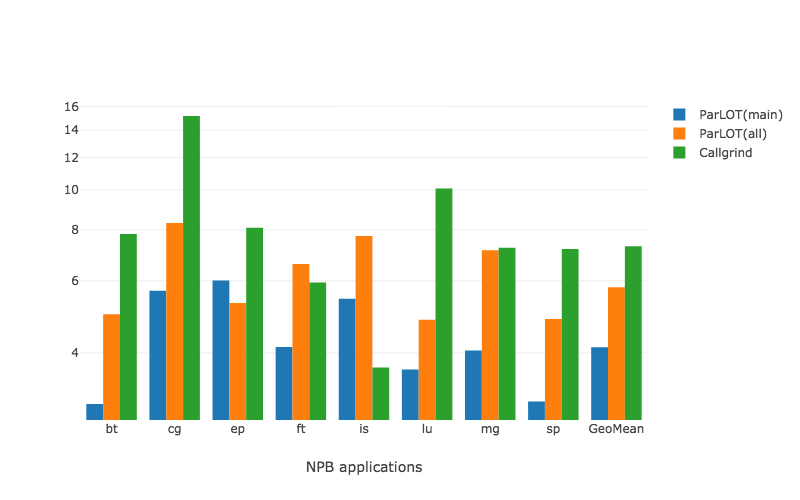
\includegraphics[width=5in]{figs.psc/chartAvg_sd_B_p3_5.png}
\caption{ Slowdown of ParLOT(main,all) and Callgrind. Each bar is the average slowdown of each tool on each application for 1, 4 and 16 nodes (16, 64 and 256 cores). Last group of bars is GeoMean (from bold numbers in table \ref{sd_pMpAcg_B_itn_p3.5}). 
}
\label{chartAvg_sd_B_p3_5}
\end{figure*}

\begin{table*}[]
\caption{Server: \textbf{Comet} - 
 Stat: \textbf{Detail Slowdown} -
 Tools: pinMain , pinAll , callgrind -  
 Inputs: B -
 Nodes: 1 , 4 , 16 , 64 -
 Desc: Primary  - Similar to table \ref{sd_pMpAcg_B_itn_p3.5} but numbers are from Comet}
\label{comet_sd_pMpAcg_B_itn_p3.5}
\begin{center}
\begin{tabular}{|l|rrrrrrrr|r|}
\hline
                &   bt &   cg &   ep &    ft &   is &   lu &   mg &   sp &   GM \\
\hline
 pinMain.B.1    & 1.55 & 1.82 & 2.68 &  2.11 & 2.48 & 1.31 & 2.57 & 1.33 & 1.91 \\
 pinMain.B.4    & 1.76 & 1.85 & 1.92 &  1.74 & 1.79 & 1.77 & 1.83 & 1.76 & 1.80 \\
 pinMain.B.16   & 2.19 & 2.62 & 2.39 &  1.93 & 1.82 & 2.80 & 2.43 & 2.23 & 2.28 \\
 pinMain.B.64   & 2.45 & 2.72 & 2.45 &  1.99 & 4.34 & 4.56 & 2.31 & 2.46 & 2.79 \\
 \hline
 AVG            & 1.99 & 2.25 & 2.36 &  1.94 & 2.61 & 2.61 & 2.29 & 1.95 & \textbf{2.20} \\
 \hline
 pinAll.B.1     & 1.85 & 2.73 & 4.21 &  2.85 & 4.52 & 1.74 & 5.57 & 1.73 & 2.87 \\
 pinAll.B.4     & 2.63 & 3.11 & 3.41 &  2.86 & 3.03 & 2.82 & 3.10 & 2.76 & 2.96 \\
 pinAll.B.16    & 3.73 & 4.20 & 4.36 &  2.96 & 2.84 & 4.30 & 4.49 & 3.71 & 3.77 \\
 pinAll.B.64    & 4.22 & 4.19 & 4.55 &  3.13 & 5.46 & 4.73 & 4.17 & 4.23 & 4.29 \\
 \hline
 AVG            & 3.11 & 3.56 & 4.13 &  2.95 & 3.96 & 3.40 & 4.33 & 3.11 & \textbf{3.47} \\
 \hline
 callgrind.B.1  & 8.68 & 6.07 & 9.31 & 10.33 & 2.64 & 7.61 & 3.39 & 6.62 & 6.24 \\
 callgrind.B.4  & 6.13 & 3.63 & 2.95 &  3.50 & 1.46 & 5.41 & 1.43 & 5.98 & 3.34 \\
 callgrind.B.16 & 4.31 & 3.26 & 2.39 &  2.20 & 1.73 & 4.70 & 1.92 & 4.65 & 2.93 \\
 callgrind.B.64 & 2.85 & 2.71 & 1.86 &  2.16 & 4.13 & 4.10 & 1.87 & 3.54 & 2.77 \\
 \hline
 AVG            & 5.49 & 3.92 & 4.13 &  4.55 & 2.49 & 5.46 & 2.15 & 5.20 & \textbf{3.82} \\
\hline
\end{tabular}
\end{center}
\end{table*}

\begin{table*}[]
\caption{Stat: sd 
 Tools: pinMain , pinAll , callgrind ,  
 Inputs: B ,  
 Nodes: 1 , 4 , 16 ,  
 Desc: Primary}
\label{ls5_sd_pMpAcg_B_itn_p3.5}\begin{center}
\begin{tabular}{lrrrrrrrrr}
\hline
                &   bt &   cg &   ep &   ft &   is &   lu &   mg &   sp &   GM \\
\hline
 pinMain.B.1    & 1.67 & 1.48 & 3.40 & 1.93 & 1.93 & 1.10 & 2.08 & 1.04 & 1.71 \\
 pinMain.B.4    & 1.63 & 1.57 & 1.69 & 2.41 & 2.33 & 1.48 & 1.53 & 3.87 & 1.95 \\
 pinMain.B.16   & 2.23 & 1.65 & 2.08 & 1.82 & 2.66 & 1.84 & 1.57 & 1.60 & 1.90 \\
 AVG            & 1.84 & 1.57 & 2.39 & 2.05 & 2.31 & 1.47 & 1.73 & 2.17 & 1.85 \\
 pinAll.B.1     & 1.97 & 2.55 & 4.15 & 2.73 & 3.71 & 1.55 & 3.96 & 1.31 & 2.53 \\
 pinAll.B.4     & 2.33 & 2.68 & 2.84 & 4.03 & 4.59 & 2.41 & 2.89 & 3.47 & 3.07 \\
 pinAll.B.16    & 4.20 & 2.68 & 4.85 & 2.71 & 8.53 & 3.34 & 2.81 & 2.98 & 3.70 \\
 AVG            & 2.83 & 2.64 & 3.95 & 3.16 & 5.61 & 2.43 & 3.22 & 2.59 & 3.10 \\
 callgrind.B.1  & 0.00 & 0.00 & 0.00 & 0.00 & 0.00 & 0.00 & 0.00 & 0.00 & 0.00 \\
 callgrind.B.4  & 0.00 & 0.00 & 0.00 & 0.00 & 0.00 & 0.00 & 0.00 & 0.00 & 0.00 \\
 callgrind.B.16 & 0.00 & 0.00 & 0.00 & 0.00 & 0.00 & 0.00 & 0.00 & 0.00 & 0.00 \\
 AVG            & 0.00 & 0.00 & 0.00 & 0.00 & 0.00 & 0.00 & 0.00 & 0.00 & 0.00 \\
\hline
\end{tabular}
\end{center}
\end{table*}



\begin{table*}[]
%\caption{Stat: bw 
% Tools: pinMain , pinAll , callgrind ,  
% Inputs: B ,  
% Nodes: 1 , 4 , 16 ,  
% Desc: Primary}


\caption{This table is showing the required bandwidth for each application (KiloBytes per core per second). $ReqBW_x = TraceSize_x (KB) / (\# of cores)_x / Runtime_x (S)$
Because of the crashing problems of Callgrind on \textit{C} input and 64 nodes, I only include \textit{B} input and 1, 4, and 16 nodes results. Clearly ParLOT(main) is beating Callgrind while they both generate the same information (I still believe ParLOT(main) generated traces are more informative and rich). ParLOT(all) bandwidth is the highest but with capturing all of the function calls within a single execution, there is no surprise. Another interesting fact from this table is, for ParLOT(main), bandwidth drops from \textbf{0.62} for 16 cores to \textbf{0.27} for 256 cores (good scalability). It is the opposite for Callgrind where the required bandwidth jumps from \textbf{3.28} (KB/s) for 16 cores to \textbf{33.06} (KB/S) for 256 cores. I also have the results of required bandwidth of ParLOT for 64 nodes(1024 cores) and Input C but I did not include them here because I did not have them for Callgrind (explained above).  Fig \ref{chartAvg_bw_B_p3_5} visualize these numbers (Average values)}
\label{bw_pMpAcg_B_itn_p3.5}
\begin{center}
\begin{tabular}{|l|rrrrrrrr|r|}
\hline
                &    bt &    cg &    ep &    ft &    is &    lu &    mg &    sp &    GM \\
\hline
 pinMain.B.1    &  2.54 & 22.73 &  0.99 &  0.33 &  0.46 &  0.10 &  0.43 &  0.06 &  0.62 \\
 pinMain.B.4    &  3.20 & 18.31 &  0.52 &  0.20 &  0.12 &  0.11 &  0.23 &  0.10 &  0.46 \\
 pinMain.B.16   &  2.20 &  9.66 &  0.09 &  0.14 &  0.06 &  0.08 &  0.19 &  0.13 &  0.27 \\
 \hline
 AVG            &  2.65 & 16.90 &  0.53 &  0.22 &  0.21 &  0.10 &  0.28 &  0.10 &  \textbf{0.45} \\
 \hline
 pinAll.B.1     & 20.80 & 39.89 & 14.75 & 21.05 & 31.00 & 19.55 & 34.37 & 12.37 & 22.53 \\
 pinAll.B.4     & 21.85 & 33.10 & 22.15 & 17.05 & 16.19 & 35.84 & 34.53 & 35.99 & 25.81 \\
 pinAll.B.16    & 25.31 & 29.33 & 23.31 & 20.07 & 23.78 & 56.58 & 29.09 & 42.96 & 29.57 \\
 \hline
 AVG            & 22.65 & 34.11 & 20.07 & 19.39 & 23.66 & 37.32 & 32.66 & 30.44 & \textbf{25.97} \\
 \hline
 callgrind.B.1  &  0.90 &  2.40 &  2.53 &  4.02 & 24.33 &  1.39 & 14.64 &  1.22 &  3.28 \\
 callgrind.B.4  &  4.27 &  9.11 & 12.02 & 16.78 & 59.03 &  2.97 & 35.78 &  5.20 & 11.25 \\
 callgrind.B.16 & 17.48 & 12.87 & 46.08 & 51.94 & 87.05 & 19.13 & 48.00 & 33.18 & 33.06 \\
 \hline
 AVG            &  7.55 &  8.13 & 20.21 & 24.25 & 56.80 &  7.83 & 32.81 & 13.20 & \textbf{15.86} \\
\hline
\end{tabular}
\end{center}
\end{table*}


\begin{figure*}[!t]
\centering
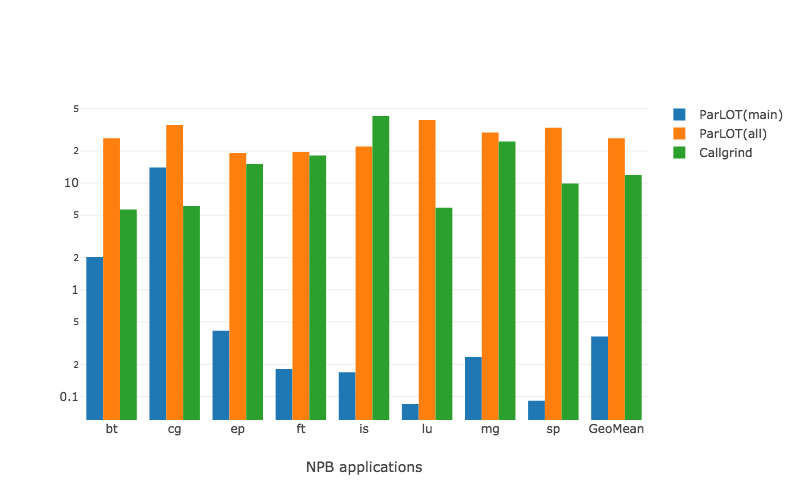
\includegraphics[width=5in]{figs.psc/chartAvg_bw_B_p3_5.png}
\caption{ Required Bandwidth (KB) per core per second for ParLOT and Callgrind.  
(Input: B)}
\label{chartAvg_bw_B_p3_5}
\end{figure*}

\begin{table*}[]
\caption{Server: \textbf{Comet} -
 Stat: \textbf{Bandwidth} -
 Tools: pinMain , pinAll , callgrind - 
 Inputs: B -
 Nodes: 1 , 4 , 16 , 64 -
 Desc: Primary}
\label{comet_bw_pMpAcg_B_itn_p3.5}\begin{center}
\begin{tabular}{|l|rrrrrrrr|r|}
\hline
                &    bt &     cg &    ep &    ft &    is &     lu &    mg &    sp &    GM \\
\hline
 pinMain.B.1    &  4.72 &  21.86 &  3.83 &  1.52 &  0.79 &   2.39 &  5.62 &  5.36 &  3.69 \\
 pinMain.B.4    & 14.28 &  41.08 &  1.89 &  3.48 &  2.24 &  21.48 &  6.45 & 15.85 &  8.12 \\
 pinMain.B.16   & 14.31 &  46.59 &  1.45 &  4.86 &  3.40 &  31.79 &  6.53 & 18.55 &  9.41 \\
 pinMain.B.64   & 18.56 &  43.59 &  1.25 &  4.56 &  4.49 &  27.07 &  5.63 & 29.62 &  9.92 \\
 \hline
 AVG            & 12.97 &  38.28 &  2.10 &  3.60 &  2.73 &  20.68 &  6.06 & 17.35 &  7.79 \\
 \hline
 pinAll.B.1     & 48.71 &  89.39 & 47.23 & 45.63 & 59.98 &  53.62 & 60.81 & 54.33 & 56.21 \\
 pinAll.B.4     & 61.84 & 101.23 & 45.21 & 55.12 & 53.20 &  71.09 & 54.85 & 73.62 & 62.68 \\
 pinAll.B.16    & 73.95 & 116.87 & 47.37 & 48.88 & 47.79 & 100.91 & 55.80 & 84.61 & 67.97 \\
 pinAll.B.64    & 81.80 & 110.15 & 44.16 & 47.98 & 37.84 & 100.26 & 52.67 & 99.90 & 66.47 \\
 \hline
 AVG            & 66.58 & 104.41 & 45.99 & 49.40 & 49.70 &  81.47 & 56.03 & 78.12 & 63.33 \\
 \hline
 callgrind.B.1  &  1.57 &   7.69 &  7.39 &  4.56 & 39.49 &   2.61 & 34.41 &  2.71 &  6.67 \\
 callgrind.B.4  &  6.51 &  16.01 & 22.10 & 15.65 & 45.46 &   8.63 & 45.47 &  7.78 & 16.31 \\
 callgrind.B.16 & 17.20 &  24.62 & 37.42 & 23.84 & 29.87 &  16.23 & 51.49 & 15.81 & 24.93 \\
 callgrind.B.64 & 26.82 &  27.65 & 45.93 & 25.14 & 11.04 &  17.75 & 45.27 & 20.20 & 25.02 \\
 \hline
 AVG            & 13.03 &  18.99 & 28.21 & 17.30 & 31.47 &  11.30 & 44.16 & 11.62 & 18.23 \\
\hline
\end{tabular}
\end{center}
\end{table*}

\begin{table*}[]
\caption{Server = \textbf{Lonestar5} - Stat: \textbf{Bandwidth} - 
 Tools: pinMain , pinAll , callgrind -  
 Inputs: B -
 Nodes: 1 , 4 , 16 -
 Desc: Primary}
\label{ls5_bw_pMpAcg_B_itn_p3.5}\begin{center}
\begin{tabular}{|l|rrrrrrrr|r|}
\hline
                &    bt &    cg &    ep &    ft &    is &     lu &    mg &     sp &    GM \\
\hline
 pinMain.B.1    &  2.35 &  0.97 &  3.18 &  1.34 &  0.24 &   0.51 &  2.05 &   3.14 &  1.29 \\
 pinMain.B.4    &  3.79 &  1.01 &  1.87 &  1.27 &  0.19 &   0.83 &  1.55 &   0.65 &  1.05 \\
 pinMain.B.16   &  2.62 &  0.95 &  0.91 &  1.11 &  0.16 &   0.81 &  1.23 &   0.98 &  0.89 \\
 \hline
 AVG            &  2.92 &  0.98 &  1.99 &  1.24 &  0.20 &   0.72 &  1.61 &   1.59 &  1.08 \\
 \hline
 pinAll.B.1     & 38.93 & 56.70 & 53.53 & 46.05 & 75.28 &  49.93 & 72.77 &  44.12 & 53.35 \\
 pinAll.B.4     & 76.90 & 86.79 & 55.27 & 57.31 & 64.06 & 107.60 & 69.93 &  99.71 & 75.14 \\
 pinAll.B.16    & 74.29 & 96.22 & 30.95 & 65.10 & 36.18 & 118.90 & 66.92 & 132.38 & 69.57 \\
 \hline
 AVG            & 63.37 & 79.90 & 46.58 & 56.15 & 58.51 &  92.14 & 69.87 &  92.07 & 66.02 \\
 \hline
 callgrind.B.1  &  0.00 &  0.00 &  0.00 &  0.00 &  0.00 &   0.00 &  0.00 &   0.00 &  0.00 \\
 callgrind.B.4  &  0.00 &  0.00 &  0.00 &  0.00 &  0.00 &   0.00 &  0.00 &   0.00 &  0.00 \\
 callgrind.B.16 &  0.00 &  0.00 &  0.00 &  0.00 &  0.00 &   0.00 &  0.00 &   0.00 &  0.00 \\
 \hline
 AVG            &  0.00 &  0.00 &  0.00 &  0.00 &  0.00 &   0.00 &  0.00 &   0.00 &  0.00 \\
\hline
\end{tabular}
\end{center}
\end{table*}



\begin{table*}[]
%\caption{Stat: cr 
% Tools: pinMain , pinAll ,  
% Inputs: C , B ,  
% Nodes: 1 , 4 , 16 , 64 ,  
% Desc: Primary}
\caption{COMPRESSION RATIOS FOR B AND C INPUTS AND 1, 4, 16 AND 64 NODES.}
\label{cr_pMpA_BC_itn_p3.5}
\begin{center}
\begin{tabular}{|l|rrrrrrrr|r|}
\hline
              &       bt &      cg &       ep &       ft &       is &       lu &      mg &       sp &      GM \\
\hline
 pinMain.C.1  & 14051.90 &   85.18 & 12104.15 & 31406.62 & 36422.85 & 20423.90 & 1169.56 & 22561.69 & 7393.79 \\
 pinMain.C.4  &  8249.54 &   85.36 & 12067.24 & 24222.90 & 33655.89 & 11191.63 &  650.18 & 10441.99 & 5189.93 \\
 pinMain.C.16 &  1985.31 &   85.55 & 11921.80 & 11426.88 & 25812.61 &  7353.92 &  353.38 &  4810.38 & 3048.85 \\
 pinMain.C.64 &   709.30 &   85.74 & 11374.25 &  6738.89 & 13360.80 &  6916.77 &  250.95 &  4624.28 & 2174.51 \\
 \hline
 AVG          &  6249.01 &   85.46 & 11866.86 & 18448.82 & 27313.04 & 11471.56 &  606.02 & 10609.58 & 4451.77 \\
 \hline
 pinAll.C.1   &  2579.37 &   89.08 & 21213.12 &  6818.31 &  7698.78 &   135.16 &   89.48 &   272.48 &  978.90 \\
 pinAll.C.4   &  1441.93 &  301.17 & 13242.06 &  1412.63 &  1122.81 &   709.17 &  857.56 &   773.11 & 1199.60 \\
 pinAll.C.16  &  1954.84 &  413.29 &  6721.88 &  1531.17 &  1793.81 &   430.15 & 1317.55 &   820.22 & 1273.86 \\
 pinAll.C.64  &  1195.58 &  891.83 &  5537.37 &  3191.36 &  2461.46 &   676.34 & 2412.46 &   967.72 & 1710.36 \\
 \hline
 AVG          &  1792.93 &  423.84 & 11678.61 &  3238.37 &  3269.22 &   487.71 & 1169.26 &   708.38 & 1290.68 \\
 \hline
 pinMain.B.1  &  5403.04 &   74.95 & 12067.06 & 12704.90 & 33655.87 &  8750.65 &  541.98 & 10426.05 & 4234.22 \\
 pinMain.B.4  &  2129.01 &   75.33 & 11922.18 & 10745.40 & 25812.57 &  5128.06 &  364.22 &  4042.15 & 2820.40 \\
 pinMain.B.16 &   729.64 &   75.70 & 11374.86 &  3508.41 & 13360.75 &  4371.76 &  205.67 &  3265.36 & 1746.25 \\
 pinMain.B.64 &  3551.97 &   76.08 &  9608.18 &  2790.59 &  4563.29 &  4031.59 &  164.19 &  4030.09 & 1750.60 \\
 \hline
 AVG          &  2953.41 &   75.52 & 11243.07 &  7437.32 & 19348.12 &  5570.52 &  319.02 &  5440.91 & 2637.87 \\
 \hline
 pinAll.B.1   &   750.27 &   68.40 & 16927.14 &  2584.15 &  2304.36 &   101.34 &   69.80 &   119.94 &  507.33 \\
 pinAll.B.4   &  1693.37 &  649.30 &  6797.11 &  2165.42 &  2402.91 &   727.52 &  836.96 &   672.73 & 1413.43 \\
 pinAll.B.16  &  1265.26 & 1138.20 &  4140.31 &  1794.78 &  1993.44 &   620.41 & 1477.61 &   883.86 & 1427.94 \\
 pinAll.B.64  &  1294.03 & 1218.33 &  5187.85 &  3086.80 &  3266.69 &  1044.65 & 2520.99 &  1167.23 & 1997.57 \\
 \hline
 AVG          &  1250.73 &  768.56 &  8263.10 &  2407.79 &  2491.85 &   623.48 & 1226.34 &   710.94 & 1336.57 \\

\hline
\end{tabular}
\end{center}
\end{table*}

\begin{table*}[]
\caption{Server: \textbf{Comet} - \textbf{COMPRESSION RATIOS} FOR B INPUTS AND 1, 4, 16 AND 64 NODES - C input experiments are cooking}
\label{comet_cr_pMpA_B_itn_p3.5}\begin{center}
\begin{tabular}{|l|rrrrrrrr|r|}
\hline
              &      bt &     cg &       ep &       ft &      is &     lu &     mg &     sp &      GM \\
\hline
 pinMain.B.1  & 3035.93 &  94.35 & 12456.18 & 12173.49 & 9718.38 & 167.72 &  99.08 & 878.27 & 1255.17 \\
 pinMain.B.4  &  586.64 &  82.48 & 10368.41 &  1737.09 &  909.20 & 140.29 & 254.95 & 338.16 &  559.36 \\
 pinMain.B.16 &  346.66 & 113.28 &  8563.85 &  1077.35 & 1200.57 & 178.98 & 387.63 & 123.02 &  496.83 \\
 pinMain.B.64 &  252.24 & 147.78 &  7611.04 &  1122.62 & 1907.95 & 366.80 & 437.31 & 152.91 &  591.11 \\
 \hline
 AVG          & 1055.37 & 109.47 &  9749.87 &  4027.64 & 3434.03 & 213.45 & 294.74 & 373.09 &  725.62 \\
 \hline
 pinAll.B.1   &  514.51 & 137.41 &  3335.77 &  1226.74 &  543.18 & 314.63 & 260.87 & 303.88 &  500.21 \\
 pinAll.B.4   &  315.71 & 137.21 &  1266.92 &   436.15 &  316.16 & 287.25 & 329.57 & 199.66 &  330.70 \\
 pinAll.B.16  &  226.86 & 181.58 &  1246.66 &  1026.53 &  927.09 & 299.30 & 469.29 & 171.52 &  430.39 \\
 pinAll.B.64  &  329.23 & 247.30 &  1394.07 &  1043.94 & 1984.62 & 410.32 & 548.47 & 307.16 &  597.55 \\
 \hline
 AVG          &  346.58 & 175.88 &  1810.86 &   933.34 &  942.76 & 327.88 & 402.05 & 245.56 &  464.71 \\
\hline
\end{tabular}
\end{center}
\end{table*}



\begin{table*}[]
%\caption{Stat: sd 
% Tools:  
% Inputs: B ,  
% Nodes: 1 , 4 , 16 , 64 ,  
% Desc: Detail Report}

\caption{Server: \textbf{PSC} - Tables \ref{det_Main_all_B_p3.5}, \ref{comet_det_Main_all_B_p3.5}, \ref{ls5_det_Main_all_B_p3.5}, \ref{det_All_all_B_p3.5}, \ref{comet_det_All_all_B_p3.5} and \ref{ls5_det_All_all_B_p3.5}  are showing the detail slowdowns added to the code by each phase of ParLOT(main and all) for input size \textit{B} on \textbf{PSC}, \textbf{Comet} and \textbf{Lonestar5}. I put my observations of all four tables over here. \textbf{npin} is just the slowdown caused by initializing Pin's routines on top of the target application without doing anything else (no instrumentation, tracing, compression and I/O.  \textbf{dpin} is almost identical to ParLOT except it stores the generated compressed traces to "/dev/null". The purpose of \textit{dpin} is to see how much of the overall overhead is because of I/O and data-related slowdowns. In \textbf{wpin}, and all collected data would be stored as is to the disk. The results of this tools shows how much efficiency our compression approach adds to ParLOT. Last row of tables shows geometric mean of each of its above values showing how much each phase of ParLOT slows down the native execution. In general, we all expect that the slowdowns of $npin < dpin < ParLOT < wpin $. But majority of numbers are not like that. I double checked the results of CHPC and Stampede and the patterns are kind of identical.  In most of the table entries (in particular for smaller number of cores), the differences between the average slowdown of \textit{dpin} and \textit{ParLOT} is very insignificant which shows that ParLOT is not an I/O-bounded tool. Figures \ref{chartDet_B_wc_byTool_p3_5} and \ref{chartDet_B_woc_byTool_p3_5} visualize numbers from these tables.} 
\label{det_Main_all_B_p3.5}

\begin{center}
\scalebox{0.95}{
\begin{tabular}{|c|c|rrrr|rrrr|rrrr|rrrr|} 
\hline 
\multicolumn{1}{|l|}{\multirow{2}{*}{\textbf{Input: B}}} & \multicolumn{1}{r|}{Nodes :}    & \multicolumn{4}{c|}{1}  & \multicolumn{4}{c|}{4} & \multicolumn{4}{c|}{16}  & \multicolumn{4}{c|}{64} \\ \cline{2-18} 
\multicolumn{1}{|l|}{} & \multicolumn{1}{r|}{Detail Tools:} & \multicolumn{1}{c}{npin} & \multicolumn{1}{c}{dpin} & \multicolumn{1}{c}{ParLOT} & \multicolumn{1}{c|}{wpin} & \multicolumn{1}{c}{npin} & \multicolumn{1}{c}{dpin} & \multicolumn{1}{c}{ParLOT} & \multicolumn{1}{c|}{wpin} & \multicolumn{1}{c}{npin} & \multicolumn{1}{c}{dpin} & \multicolumn{1}{c}{ParLOT} & \multicolumn{1}{c|}{wpin} & \multicolumn{1}{c}{npin} & \multicolumn{1}{c}{dpin} & \multicolumn{1}{c}{ParLOT} & \multicolumn{1}{c|}{wpin} \\
\hline
\multirow{9}{*}{Main} &  bt  &  1.49  &  1.52  &  1.60  &  11.63  &  1.17  &  1.58  &  1.67  &  8.53  &  1.86  &  2.99  &  3.68  &   8.81  &  4.22  &  4.51  &   5.07  &  13.64 \\
 &  cg  &  1.78  & \cellcolor{blue!25} 1.76  &  1.81  &   3.19  &  2.64  &  5.02  & \cellcolor{blue!25} 3.78  &  6.76  &  4.86  &  6.27  &  7.80  &  12.38  &  3.92  &  8.43  &   9.31  &  12.96 \\
 &  ep  &  3.82  & \cellcolor{blue!25} 3.37  &  3.93  &  22.47  &  1.84  &  2.26  &  2.43  &  7.94  &  4.97  &  5.02  &  9.90  & \cellcolor{blue!25}  9.09  &  3.27  &  7.22  &   7.78  &   7.67 \\
 &  ft  &  1.60  & \cellcolor{blue!25} 1.51  &  1.53  &   3.23  &  2.43  &  4.36  & \cellcolor{blue!25} 2.91  &  4.31  &  3.52  &  5.90  & \cellcolor{blue!25} 5.45  &   5.87  &  3.24  &  6.87  & \cellcolor{blue!25}  6.67  &   6.69 \\
 &  is  &  3.61  & \cellcolor{blue!25} 3.55  & \cellcolor{blue!25} 3.05  &  14.60  &  3.20  &  3.68  &  4.04  &  5.88  &  3.85  &  4.82  & \cellcolor{blue!25} 4.41  &   4.67  &  4.80  &  9.99  &  10.19  &  10.46 \\
 &  lu  &  1.39  & \cellcolor{blue!25} 1.20  &  1.21  &   1.58  &  1.85  &  2.07  &  2.83  &  3.52  &  1.64  &  3.00  &  3.81  &   5.53  &  3.17  &  6.77  & \cellcolor{blue!25}  6.73  &  13.70 \\
 &  mg  &  3.91  & \cellcolor{blue!25} 3.51  &  3.61  &   3.84  &  3.19  &  3.34  &  3.54  &  3.96  &  2.95  &  3.36  &  3.51  &   3.82  &  3.70  &  5.57  & \cellcolor{blue!25}  5.56  &   5.70 \\
 &  sp  &  1.25  &  1.43  &  1.53  &   1.65  &  2.13  &  4.38  & \cellcolor{blue!25} 2.93  &  3.63  &  2.98  &  3.48  & \cellcolor{blue!25} 2.41  &   3.86  &  4.28  &  5.78  & \cellcolor{blue!25}  5.30  &   8.56 \\ \cline{2-18}
 &  GM  &  2.11  & \cellcolor{blue!25} 2.03  &  2.08  &   5.00  &  2.20  &  3.11  & \cellcolor{blue!25} 2.92  &  5.26  &  3.11  &  4.18  &  4.65  &   6.21  &  3.79  &  6.71  &   6.87  &   9.45 \\
\hline 
\end{tabular} }

\end{center}
\end{table*}









\begin{table*}[]
\caption{Server: \textbf{Comet} - 
 Stat: \textbf{Detail Slowdown} -
 Inputs: B -
 Nodes: 1 , 4 , 16 , 64 -
 Desc: Detail Report}
\begin{center}
\label{comet_det_Main_all_B_p3.5}
\scalebox{0.95}{
\begin{tabular}{|c|c|rrrr|rrrr|rrrr|rrrr|} 
\hline 
\multicolumn{1}{|l|}{\multirow{2}{*}{\textbf{Input: B}}} & \multicolumn{1}{r|}{Nodes :}    & \multicolumn{4}{c|}{1}  & \multicolumn{4}{c|}{4} & \multicolumn{4}{c|}{16}  & \multicolumn{4}{c|}{64} \\ \cline{2-18} 
\multicolumn{1}{|l|}{} & \multicolumn{1}{r|}{Detail Tools:} & \multicolumn{1}{c}{npin} & \multicolumn{1}{c}{dpin} & \multicolumn{1}{c}{ParLOT} & \multicolumn{1}{c|}{wpin} & \multicolumn{1}{c}{npin} & \multicolumn{1}{c}{dpin} & \multicolumn{1}{c}{ParLOT} & \multicolumn{1}{c|}{wpin} & \multicolumn{1}{c}{npin} & \multicolumn{1}{c}{dpin} & \multicolumn{1}{c}{ParLOT} & \multicolumn{1}{c|}{wpin} & \multicolumn{1}{c}{npin} & \multicolumn{1}{c}{dpin} & \multicolumn{1}{c}{ParLOT} & \multicolumn{1}{c|}{wpin} \\
\hline
\multirow{9}{*}{Main} &  bt  &  1.50  &  1.56  & \cellcolor{blue!25} 1.55  &   5.66  &  1.74  &  1.79  & \cellcolor{blue!25} 1.76  &  5.19  &  2.21  & \cellcolor{blue!25} 2.13  &  2.19  &  11.49  &  2.29  &  2.48  & \cellcolor{blue!25} 2.45  &  17.89 \\
 &  cg  &  1.75  &  1.87  & \cellcolor{blue!25} 1.82  &   2.39  &  1.95  & \cellcolor{blue!25} 1.84  &  1.85  &  2.64  &  2.72  & \cellcolor{blue!25} 2.52  &  2.62  &  12.39  &  2.67  & \cellcolor{blue!25} 2.35  &  2.72  &  22.61 \\
 &  ep  &  2.97  & \cellcolor{blue!25} 2.74  & \cellcolor{blue!25} 2.68  &  21.44  &  2.07  & \cellcolor{blue!25} 1.90  &  1.92  &  5.82  &  2.58  & \cellcolor{blue!25} 2.34  &  2.39  &   4.22  &  2.81  & \cellcolor{blue!25} 2.52  & \cellcolor{blue!25} 2.45  &   3.28 \\
 &  ft  &  1.87  &  2.10  &  2.11  &   6.29  &  1.76  &  1.76  & \cellcolor{blue!25} 1.74  &  2.85  &  2.13  & \cellcolor{blue!25} 1.88  &  1.93  &   2.59  &  2.23  & \cellcolor{blue!25} 1.89  &  1.99  &   2.34 \\
 &  is  &  2.51  &  2.54  & \cellcolor{blue!25} 2.48  &   4.87  &  1.80  & \cellcolor{blue!25} 1.78  &  1.79  &  2.08  &  2.11  & \cellcolor{blue!25} 1.76  &  1.82  &   2.24  &  4.76  & \cellcolor{blue!25} 4.31  &  4.34  &   6.29 \\
 &  lu  &  1.32  & \cellcolor{blue!25} 1.31  &  1.31  &   1.44  &  1.77  &  1.78  & \cellcolor{blue!25} 1.77  &  2.27  &  2.74  & \cellcolor{blue!25} 2.66  &  2.80  &   4.06  &  3.05  & \cellcolor{blue!25} 2.81  &  4.56  &   7.94 \\
 &  mg  &  2.64  & \cellcolor{blue!25} 2.62  & \cellcolor{blue!25} 2.57  &   2.80  &  1.75  & \cellcolor{blue!25} 1.69  &  1.83  &  1.79  &  2.64  & \cellcolor{blue!25} 2.36  &  2.43  &   3.23  &  2.37  & \cellcolor{blue!25} 2.15  &  2.31  &   2.81 \\
 &  sp  &  1.35  &  1.35  & \cellcolor{blue!25} 1.33  &   2.47  &  1.74  &  1.76  &  1.76  &  3.72  &  2.15  & \cellcolor{blue!25} 2.03  &  2.23  &   2.94  &  2.29  & \cellcolor{blue!25} 2.18  &  2.46  &   6.84 \\ \cline{2-18}
 &  GM  &  1.90  &  1.94  & \cellcolor{blue!25} 1.91  &   4.15  &  1.82  & \cellcolor{blue!25} 1.79  &  1.80  &  3.03  &  2.40  & \cellcolor{blue!25} 2.19  &  2.28  &   4.38  &  2.72  & \cellcolor{blue!25} 2.51  &  2.79  &   6.45 \\
\hline 
\end{tabular} }

\end{center}
\end{table*}

\begin{table*}[]
\caption{Stat: sd 
 Tools:  
 Inputs: B ,  
 Nodes: 1 , 4 , 16 , 64 ,  
 Desc: Detail Report}
\begin{center}
\label{ls5_det_Main_all_B_p3.5}
\scalebox{0.95}{
\begin{tabular}{|c|c|rrrr|rrrr|rrrr|rrrr|} 
\hline 
\multicolumn{1}{|l|}{\multirow{2}{*}{\textbf{Input: B}}} & \multicolumn{1}{r|}{Nodes :}    & \multicolumn{4}{c|}{1}  & \multicolumn{4}{c|}{4} & \multicolumn{4}{c|}{16}  & \multicolumn{4}{c|}{64} \\ \cline{2-18} 
\multicolumn{1}{|l|}{} & \multicolumn{1}{r|}{Detail Tools:} & \multicolumn{1}{c}{npin} & \multicolumn{1}{c}{dpin} & \multicolumn{1}{c}{ParLOT} & \multicolumn{1}{c|}{wpin} & \multicolumn{1}{c}{npin} & \multicolumn{1}{c}{dpin} & \multicolumn{1}{c}{ParLOT} & \multicolumn{1}{c|}{wpin} & \multicolumn{1}{c}{npin} & \multicolumn{1}{c}{dpin} & \multicolumn{1}{c}{ParLOT} & \multicolumn{1}{c|}{wpin} & \multicolumn{1}{c}{npin} & \multicolumn{1}{c}{dpin} & \multicolumn{1}{c}{ParLOT} & \multicolumn{1}{c|}{wpin} \\
\hline
\multirow{9}{*}{Main} &  bt  &  2.11  & \cellcolor{blue!25} 1.67  &  1.67  &   6.86  &  1.24  &  1.57  &  1.63  &  9.99  &  1.25  &  2.18  &  2.23  &  6.96  &  2.38  &  2.54  &  2.59  &  3.26 \\
 &  cg  &  1.50  &  2.85  & \cellcolor{blue!25} 1.48  &   3.33  &  1.46  &  2.71  & \cellcolor{blue!25} 1.57  &  3.28  &  2.25  &  2.80  & \cellcolor{blue!25} 1.65  &  4.32  &  2.54  &  2.73  & \cellcolor{blue!25} 2.64  &  3.55 \\
 &  ep  &  3.09  &  3.92  & \cellcolor{blue!25} 3.40  &  16.33  &  1.49  &  1.63  &  1.69  &  7.96  &  1.60  &  2.24  & \cellcolor{blue!25} 2.08  &  3.75  &  2.11  &  2.28  & \cellcolor{blue!25} 2.04  &  2.69 \\
 &  ft  &  1.58  &  1.91  &  1.93  &   8.71  &  2.19  &  2.90  & \cellcolor{blue!25} 2.41  &  6.75  &  2.24  &  2.28  & \cellcolor{blue!25} 1.82  &  3.94  &  2.73  & \cellcolor{blue!25} 2.46  &  2.59  &  2.49 \\
 &  is  &  2.01  &  3.00  & \cellcolor{blue!25} 1.93  &   2.03  &  2.35  & \cellcolor{blue!25} 2.32  &  2.33  &  4.60  &  2.41  &  3.88  & \cellcolor{blue!25} 2.66  &  5.24  &  2.33  & \cellcolor{blue!25} 2.26  &  2.38  &  2.31 \\
 &  lu  &  1.16  &  1.23  & \cellcolor{blue!25} 1.10  &   1.21  &  1.71  &  2.72  & \cellcolor{blue!25} 1.48  &  2.58  &  2.50  &  2.83  & \cellcolor{blue!25} 1.84  &  3.05  &  2.61  & \cellcolor{blue!25} 2.54  &  2.69  &  3.11 \\
 &  mg  &  2.25  & \cellcolor{blue!25} 2.05  &  2.08  &   4.22  &  1.38  &  2.40  & \cellcolor{blue!25} 1.53  &  2.71  &  2.09  &  2.45  & \cellcolor{blue!25} 1.57  &  3.04  &  3.04  & \cellcolor{blue!25} 2.87  & \cellcolor{blue!25} 2.41  &  3.09 \\
 &  sp  &  0.98  &  1.80  & \cellcolor{blue!25} 1.04  &   3.26  &  1.89  &  2.11  &  3.87  &  8.24  &  2.49  &  2.49  & \cellcolor{blue!25} 1.60  &  2.81  &  2.82  & \cellcolor{blue!25} 2.58  &  2.82  &  2.82 \\
 &  GM  &  1.73  &  2.17  & \cellcolor{blue!25} 1.71  &   4.27  &  1.67  &  2.24  & \cellcolor{blue!25} 1.95  &  5.11  &  2.05  &  2.60  & \cellcolor{blue!25} 1.90  &  3.96  &  2.55  & \cellcolor{blue!25} 2.53  & \cellcolor{blue!25} 2.51  &  2.89 \\
\hline 
\end{tabular} }

\end{center}
\end{table*}


\begin{table*}[]
\caption{Input: B ,  All}
\label{det_All_all_B_p3.5}
\begin{center}
\scalebox{0.95}{
\begin{tabular}{|c|c|rrrr|rrrr|rrrr|rrrr|} 
\hline 
\multicolumn{1}{|l|}{\multirow{2}{*}{\textbf{Input: B}}} & \multicolumn{1}{r|}{Nodes :}    & \multicolumn{4}{c|}{1}  & \multicolumn{4}{c|}{4} & \multicolumn{4}{c|}{16}  & \multicolumn{4}{c|}{64} \\ \cline{2-18} 
\multicolumn{1}{|l|}{} & \multicolumn{1}{r|}{Detail Tools:} & \multicolumn{1}{c}{npin} & \multicolumn{1}{c}{dpin} & \multicolumn{1}{c}{ParLOT} & \multicolumn{1}{c|}{wpin} & \multicolumn{1}{c}{npin} & \multicolumn{1}{c}{dpin} & \multicolumn{1}{c}{ParLOT} & \multicolumn{1}{c|}{wpin} & \multicolumn{1}{c}{npin} & \multicolumn{1}{c}{dpin} & \multicolumn{1}{c}{ParLOT} & \multicolumn{1}{c|}{wpin} & \multicolumn{1}{c}{npin} & \multicolumn{1}{c}{dpin} & \multicolumn{1}{c}{ParLOT} & \multicolumn{1}{c|}{wpin} \\
\hline
\multirow{9}{*}{All} &  bt  &  1.79  & \cellcolor{blue!25} 1.74  &  2.01  &   9.85  &  1.65  &   1.80  &   3.95  &  11.66  &   2.82  &   4.91  &   6.55  &  19.22  &  5.53  &  7.54  & \cellcolor{blue!25} 7.38  &  35.77 \\
 &  cg  &  3.41  & \cellcolor{blue!25} 2.76  &  3.03  &   5.50  &  4.47  &   4.54  &   8.96  &  15.72  &   6.74  &  10.29  &  12.53  &  26.52  &  5.35  &  7.62  &  8.72  &  28.50 \\
 &  ep  &  4.85  & \cellcolor{blue!25} 4.46  &  4.63  &  71.39  &  3.06  &   3.27  &   3.52  &  23.90  &  10.03  &  10.18  & \cellcolor{blue!25}  6.47  &  19.03  &  4.96  &  5.46  &  6.58  &  11.81 \\
 &  ft  &  2.40  & \cellcolor{blue!25} 2.31  &  2.43  &   7.40  &  4.09  & \cellcolor{blue!25}  4.08  &   7.67  &  10.68  &   5.63  &   6.23  &  10.40  &  15.70  &  5.97  & \cellcolor{blue!25} 5.42  &  5.88  &  17.76 \\
 &  is  &  7.07  & \cellcolor{blue!25} 6.35  &  6.86  &  21.77  &  5.50  & \cellcolor{blue!25}  5.40  &  10.25  & \cellcolor{blue!25} 10.21  &   7.04  & \cellcolor{blue!25}  4.25  &   5.45  &   8.92  &  8.73  & \cellcolor{blue!25} 6.01  &  8.31  &  19.58 \\
 &  lu  &  1.73  & \cellcolor{blue!25} 1.55  &  1.66  &   2.75  &  2.76  &   5.27  &   5.83  &  14.45  &   4.34  & \cellcolor{blue!25}  2.55  &   4.01  &  26.05  &  6.39  & \cellcolor{blue!25} 4.49  &  7.78  &  83.68 \\
 &  mg  &  8.60  & \cellcolor{blue!25} 8.32  &  9.10  &  11.11  &  5.80  &  10.41  & \cellcolor{blue!25}  6.18  &  10.42  &   5.22  & \cellcolor{blue!25}  5.05  &   6.35  &  14.75  &  7.95  & \cellcolor{blue!25} 5.97  &  6.88  &  21.89 \\
 &  sp  &  1.50  &  1.50  &  1.56  &   3.09  &  3.07  &   5.66  & \cellcolor{blue!25}  3.70  &   8.43  &   5.38  & \cellcolor{blue!25}  3.06  &   4.73  &  17.85  &  5.29  &  6.31  &  9.37  &  57.42 \\ \cline{2-18}
 &  GM  &  3.21  & \cellcolor{blue!25} 2.97  &  3.20  &   9.36  &  3.55  &   4.55  &   5.81  &  12.53  &   5.57  & \cellcolor{blue!25}  5.20  &   6.61  &  17.63  &  6.15  & \cellcolor{blue!25} 6.02  &  7.53  &  28.54 \\
\hline 
\end{tabular} }

\end{center}
\end{table*}

\begin{table*}[]
\caption{Server: \textbf{Comet} - 
 Stat: \textbf{Detail Slowdown} -
 Inputs: B -
 Nodes: 1 , 4 , 16 , 64 -
 Desc: Detail Report}
\begin{center}
\label{comet_det_All_all_B_p3.5}
\scalebox{0.95}{
\begin{tabular}{|c|c|rrrr|rrrr|rrrr|rrrr|} 
\hline 
\multicolumn{1}{|l|}{\multirow{2}{*}{\textbf{Input: B}}} & \multicolumn{1}{r|}{Nodes :}    & \multicolumn{4}{c|}{1}  & \multicolumn{4}{c|}{4} & \multicolumn{4}{c|}{16}  & \multicolumn{4}{c|}{64} \\ \cline{2-18} 
\multicolumn{1}{|l|}{} & \multicolumn{1}{r|}{Detail Tools:} & \multicolumn{1}{c}{npin} & \multicolumn{1}{c}{dpin} & \multicolumn{1}{c}{ParLOT} & \multicolumn{1}{c|}{wpin} & \multicolumn{1}{c}{npin} & \multicolumn{1}{c}{dpin} & \multicolumn{1}{c}{ParLOT} & \multicolumn{1}{c|}{wpin} & \multicolumn{1}{c}{npin} & \multicolumn{1}{c}{dpin} & \multicolumn{1}{c}{ParLOT} & \multicolumn{1}{c|}{wpin} & \multicolumn{1}{c}{npin} & \multicolumn{1}{c}{dpin} & \multicolumn{1}{c}{ParLOT} & \multicolumn{1}{c|}{wpin} \\
\hline
\multirow{9}{*}{All} &  bt  &  1.76  &  1.83  &  1.85  &   6.23  &  2.39  &  2.61  &  2.63  &  6.39  &  3.40  &  3.68  &  3.73  &  13.66  &  3.74  &  3.76  &  4.22  &  10.66 \\
 &  cg  &  2.72  & \cellcolor{blue!25} 2.69  &  2.73  &   3.80  &  2.88  &  3.08  &  3.11  &  4.64  &  4.08  &  4.08  &  4.20  &  17.58  &  4.10  & \cellcolor{blue!25} 3.97  &  4.19  &  16.54 \\
 &  ep  &  4.42  &  4.42  & \cellcolor{blue!25} 4.21  &  23.24  &  3.25  &  3.35  &  3.41  &  7.16  &  4.27  &  4.33  &  4.36  &   6.22  &  4.43  & \cellcolor{blue!25} 4.28  &  4.55  &   5.19 \\
 &  ft  &  2.82  &  2.85  &  2.85  &   6.98  &  2.65  &  2.78  &  2.86  &  3.85  &  2.96  & \cellcolor{blue!25} 2.89  &  2.96  &   6.43  &  3.60  & \cellcolor{blue!25} 3.07  &  3.13  &   3.94 \\
 &  is  &  4.67  & \cellcolor{blue!25} 4.52  &  4.52  &   7.14  &  2.89  &  3.07  & \cellcolor{blue!25} 3.03  &  3.45  &  3.02  & \cellcolor{blue!25} 2.82  &  2.84  &   6.56  &  5.43  & \cellcolor{blue!25} 5.29  &  5.46  &  14.95 \\
 &  lu  &  1.71  &  1.74  &  1.74  &   2.41  &  2.54  &  2.65  &  2.82  &  4.91  &  4.09  &  4.28  &  4.30  &  16.40  &  4.48  & \cellcolor{blue!25} 4.32  &  4.73  &  30.30 \\
 &  mg  &  4.93  &  5.07  &  5.57  &   5.66  &  2.80  &  2.97  &  3.10  &  3.17  &  4.35  &  4.43  &  4.49  &  11.40  &  3.98  &  4.03  &  4.17  &  14.96 \\
 &  sp  &  1.70  &  1.72  &  1.73  &   3.13  &  2.54  &  2.64  &  2.76  &  5.32  &  3.43  &  3.62  &  3.71  &  14.13  &  3.66  &  3.76  &  4.23  &  27.49 \\ \cline{2-18}
 &  GM  &  2.82  &  2.84  &  2.87  &   5.74  &  2.73  &  2.88  &  2.96  &  4.69  &  3.66  &  3.72  &  3.77  &  10.66  &  4.14  & \cellcolor{blue!25} 4.02  &  4.29  &  12.69 \\
\hline 
\end{tabular} }

\end{center}
\end{table*}

\begin{table*}[]
\caption{Server = \textbf{Lonestar5} - Stat: \textbf{Detail Slowdown} - 
 Inputs: B -
 Nodes: 1 , 4 , 16 , 64 -
 Desc: Detail Report}
\begin{center}
\label{ls5_det_All_all_B_p3.5}
\scalebox{0.95}{
\begin{tabular}{|c|c|rrrr|rrrr|rrrr|rrrr|} 
\hline 
\multicolumn{1}{|l|}{\multirow{2}{*}{\textbf{Input: B}}} & \multicolumn{1}{r|}{Nodes :}    & \multicolumn{4}{c|}{1}  & \multicolumn{4}{c|}{4} & \multicolumn{4}{c|}{16}  & \multicolumn{4}{c|}{64} \\ \cline{2-18} 
\multicolumn{1}{|l|}{} & \multicolumn{1}{r|}{Detail Tools:} & \multicolumn{1}{c}{npin} & \multicolumn{1}{c}{dpin} & \multicolumn{1}{c}{ParLOT} & \multicolumn{1}{c|}{wpin} & \multicolumn{1}{c}{npin} & \multicolumn{1}{c}{dpin} & \multicolumn{1}{c}{ParLOT} & \multicolumn{1}{c|}{wpin} & \multicolumn{1}{c}{npin} & \multicolumn{1}{c}{dpin} & \multicolumn{1}{c}{ParLOT} & \multicolumn{1}{c|}{wpin} & \multicolumn{1}{c}{npin} & \multicolumn{1}{c}{dpin} & \multicolumn{1}{c}{ParLOT} & \multicolumn{1}{c|}{wpin} \\
\hline
\multirow{9}{*}{All} &  bt  &  1.53  &  1.97  &  1.97  &   9.39  &  2.17  &  2.30  &  2.33  &  33.46  &  3.45  &  4.12  &  4.20  &   72.18  &  4.20  &  4.59  &  5.28  &   0.00 \\
 &  cg  &  2.14  &  2.29  &  2.55  &   4.05  &  2.82  &  4.97  & \cellcolor{blue!25} 2.68  &  43.98  &  4.43  &  4.81  & \cellcolor{blue!25} 2.68  &  149.23  &  4.28  &  4.93  & \cellcolor{blue!25} 4.91  &   0.00 \\
 &  ep  &  4.02  &  4.78  & \cellcolor{blue!25} 4.15  &  16.34  &  2.92  &  3.02  & \cellcolor{blue!25} 2.84  &   9.24  &  4.19  &  4.74  &  4.85  &    6.41  &  4.24  &  4.74  & \cellcolor{blue!25} 4.01  &  25.39 \\
 &  ft  &  2.64  &  2.72  &  2.73  &   5.39  &  4.03  & \cellcolor{blue!25} 3.98  &  4.03  &  12.50  &  4.54  &  4.90  & \cellcolor{blue!25} 2.71  &    9.93  &  4.40  &  4.79  &  5.02  &  68.34 \\
 &  is  &  3.58  &  4.17  & \cellcolor{blue!25} 3.71  &   8.37  &  4.31  &  8.59  & \cellcolor{blue!25} 4.59  &  12.97  &  7.73  & \cellcolor{blue!25} 4.51  &  8.53  &   20.20  &  4.40  &  4.41  & \cellcolor{blue!25} 4.37  &  55.11 \\
 &  lu  &  1.50  &  1.56  & \cellcolor{blue!25} 1.55  &   2.63  &  2.41  & \cellcolor{blue!25} 2.36  &  2.41  &  31.25  &  4.51  &  5.18  & \cellcolor{blue!25} 3.34  &  104.27  &  4.34  &  5.08  &  6.09  &   0.00 \\
 &  mg  &  3.76  &  3.92  &  3.96  &   7.23  &  5.16  & \cellcolor{blue!25} 3.08  & \cellcolor{blue!25} 2.89  &  29.48  &  4.72  & \cellcolor{blue!25} 2.72  &  2.81  &   37.70  &  4.99  &  5.52  & \cellcolor{blue!25} 4.82  &   0.00 \\
 &  sp  &  1.24  &  1.31  &  1.31  &   8.92  &  5.60  &  6.24  & \cellcolor{blue!25} 3.47  &  24.00  &  4.55  &  4.98  & \cellcolor{blue!25} 2.98  &  107.64  &  4.24  &  4.56  &  6.31  &   0.00 \\ \cline{2-18}
 &  GM  &  2.33  &  2.58  & \cellcolor{blue!25} 2.53  &   6.83  &  3.48  &  3.90  & \cellcolor{blue!25} 3.07  &  21.68  &  4.65  & \cellcolor{blue!25} 4.42  & \cellcolor{blue!25} 3.70  &   39.44  &  4.38  &  4.82  &  5.05  &   0.00 \\
\hline 
\end{tabular} }

\end{center}
\end{table*}



\begin{table*}[]
\caption{Server: \textbf{Comet} - 
 Stat: \textbf{Detail Slowdown  including apin(fwrite(,,0,))} -
 Inputs: B -
 Nodes: 1 , 4 , 16 , 64 -
 Desc: Detail Report 2}
\begin{center}
\label{comet_det_Main_all_B2_p3.5}
\scalebox{0.8}{
\begin{tabular}{|c|c|rrrrr|rrrrr|rrrrr|rrrrr|} 
\hline 
\multicolumn{1}{|l|}{\multirow{2}{*}{\textbf{Input: B}}} & \multicolumn{1}{r|}{Nodes :}    & \multicolumn{5}{c|}{1}  & \multicolumn{5}{c|}{4} & \multicolumn{5}{c|}{16}  & \multicolumn{5}{c|}{64} \\ \cline{2-22} 
\multicolumn{1}{|l|}{} & \multicolumn{1}{r|}{Detail Tools:} & \multicolumn{1}{c}{npin} & \multicolumn{1}{c}{apin} & \multicolumn{1}{c}{dpin} & \multicolumn{1}{c}{ParLOT} & \multicolumn{1}{c|}{wpin} & \multicolumn{1}{c}{npin} & \multicolumn{1}{c}{apin} & \multicolumn{1}{c}{dpin} & \multicolumn{1}{c}{ParLOT} & \multicolumn{1}{c|}{wpin} & \multicolumn{1}{c}{npin} & \multicolumn{1}{c}{apin} & \multicolumn{1}{c}{dpin} & \multicolumn{1}{c}{ParLOT} & \multicolumn{1}{c|}{wpin} & \multicolumn{1}{c}{npin} & \multicolumn{1}{c}{apin} & \multicolumn{1}{c}{dpin} & \multicolumn{1}{c}{ParLOT} & \multicolumn{1}{c|}{wpin} \\
\hline
\multirow{9}{*}{Main} &  bt  &  1.50  &  1.56  &  1.56  & \cellcolor{blue!25} 1.55  &   5.66  &  1.74  &  1.78  &  1.79  & \cellcolor{blue!25} 1.76  &  5.19  &  2.21  &  2.25  & \cellcolor{blue!25} 2.13  &  2.19  &  11.49  &  2.29  &  2.50  & \cellcolor{blue!25} 2.48  & \cellcolor{blue!25} 2.45  &  17.89 \\
 &  cg  &  1.75  &  1.81  &  1.87  & \cellcolor{blue!25} 1.82  &   2.39  &  1.95  & \cellcolor{blue!25} 1.84  &  1.84  &  1.85  &  2.64  &  2.72  &  2.72  & \cellcolor{blue!25} 2.52  &  2.62  &  12.39  &  2.67  & \cellcolor{blue!25} 2.53  & \cellcolor{blue!25} 2.35  &  2.72  &  22.61 \\
 &  ep  &  2.97  & \cellcolor{blue!25} 2.69  &  2.74  & \cellcolor{blue!25} 2.68  &  21.44  &  2.07  & \cellcolor{blue!25} 1.91  & \cellcolor{blue!25} 1.90  &  1.92  &  5.82  &  2.58  & \cellcolor{blue!25} 2.38  & \cellcolor{blue!25} 2.34  &  2.39  &   4.22  &  2.81  & \cellcolor{blue!25} 2.50  &  2.52  & \cellcolor{blue!25} 2.45  &   3.28 \\
 &  ft  &  1.87  &  2.11  & \cellcolor{blue!25} 2.10  &  2.11  &   6.29  &  1.76  & \cellcolor{blue!25} 1.74  &  1.76  & \cellcolor{blue!25} 1.74  &  2.85  &  2.13  & \cellcolor{blue!25} 1.85  &  1.88  &  1.93  &   2.59  &  2.23  & \cellcolor{blue!25} 1.96  & \cellcolor{blue!25} 1.89  &  1.99  &   2.34 \\
 &  is  &  2.51  & \cellcolor{blue!25} 2.47  &  2.54  & \cellcolor{blue!25} 2.48  &   4.87  &  1.80  &  1.81  & \cellcolor{blue!25} 1.78  &  1.79  &  2.08  &  2.11  & \cellcolor{blue!25} 1.86  & \cellcolor{blue!25} 1.76  &  1.82  &   2.24  &  4.76  & \cellcolor{blue!25} 4.31  &  4.31  &  4.34  &   6.29 \\
 &  lu  &  1.32  & \cellcolor{blue!25} 1.31  &  1.31  &  1.31  &   1.44  &  1.77  & \cellcolor{blue!25} 1.76  &  1.78  & \cellcolor{blue!25} 1.77  &  2.27  &  2.74  & \cellcolor{blue!25} 2.65  &  2.66  &  2.80  &   4.06  &  3.05  & \cellcolor{blue!25} 2.90  & \cellcolor{blue!25} 2.81  &  4.56  &   7.94 \\
 &  mg  &  2.64  & \cellcolor{blue!25} 2.59  &  2.62  & \cellcolor{blue!25} 2.57  &   2.80  &  1.75  & \cellcolor{blue!25} 1.72  & \cellcolor{blue!25} 1.69  &  1.83  &  1.79  &  2.64  & \cellcolor{blue!25} 2.41  & \cellcolor{blue!25} 2.36  &  2.43  &   3.23  &  2.37  &  2.44  & \cellcolor{blue!25} 2.15  &  2.31  &   2.81 \\
 &  sp  &  1.35  & \cellcolor{blue!25} 1.34  &  1.35  & \cellcolor{blue!25} 1.33  &   2.47  &  1.74  &  1.78  & \cellcolor{blue!25} 1.76  &  1.76  &  3.72  &  2.15  & \cellcolor{blue!25} 2.07  & \cellcolor{blue!25} 2.03  &  2.23  &   2.94  &  2.29  &  2.46  & \cellcolor{blue!25} 2.18  &  2.46  &   6.84 \\ \cline{2-22}
 &  GM  &  1.90  &  1.91  &  1.94  & \cellcolor{blue!25} 1.91  &   4.15  &  1.82  & \cellcolor{blue!25} 1.79  &  1.79  &  1.80  &  3.03  &  2.40  & \cellcolor{blue!25} 2.25  & \cellcolor{blue!25} 2.19  &  2.28  &   4.38  &  2.72  & \cellcolor{blue!25} 2.64  & \cellcolor{blue!25} 2.51  &  2.79  &   6.45 \\
\hline 
\end{tabular} }

\end{center}
\end{table*}



\begin{table*}[]
\caption{Server: \textbf{Comet} -
 Stat: \textbf{Detail Slowdowns including apin(fwrite(,,0,))} -
 Inputs: B -
 Nodes: 1 , 4 , 16 , 64 -
 Desc: Detail Report 2}
\begin{center}
\label{comet_det_All_all_B2_p3.5}
\scalebox{0.8}{
\begin{tabular}{|c|c|rrrrr|rrrrr|rrrrr|rrrrr|} 
\hline 
\multicolumn{1}{|l|}{\multirow{2}{*}{\textbf{Input: B}}} & \multicolumn{1}{r|}{Nodes :}    & \multicolumn{5}{c|}{1}  & \multicolumn{5}{c|}{4} & \multicolumn{5}{c|}{16}  & \multicolumn{5}{c|}{64} \\ \cline{2-22} 
\multicolumn{1}{|l|}{} & \multicolumn{1}{r|}{Detail Tools:} & \multicolumn{1}{c}{npin} & \multicolumn{1}{c}{apin} & \multicolumn{1}{c}{dpin} & \multicolumn{1}{c}{ParLOT} & \multicolumn{1}{c|}{wpin} & \multicolumn{1}{c}{npin} & \multicolumn{1}{c}{apin} & \multicolumn{1}{c}{dpin} & \multicolumn{1}{c}{ParLOT} & \multicolumn{1}{c|}{wpin} & \multicolumn{1}{c}{npin} & \multicolumn{1}{c}{apin} & \multicolumn{1}{c}{dpin} & \multicolumn{1}{c}{ParLOT} & \multicolumn{1}{c|}{wpin} & \multicolumn{1}{c}{npin} & \multicolumn{1}{c}{apin} & \multicolumn{1}{c}{dpin} & \multicolumn{1}{c}{ParLOT} & \multicolumn{1}{c|}{wpin} \\
\hline
\multirow{9}{*}{All} &  bt  &  1.76  &  1.86  & \cellcolor{blue!25} 1.83  &  1.85  &   6.23  &  2.39  &  2.59  &  2.61  &  2.63  &  6.39  &  3.40  &  3.69  & \cellcolor{blue!25} 3.68  &  3.73  &  13.66  &  3.74  &  3.98  & \cellcolor{blue!25} 3.76  &  4.22  &  10.66 \\
 &  cg  &  2.72  &  2.72  & \cellcolor{blue!25} 2.69  &  2.73  &   3.80  &  2.88  &  2.96  &  3.08  &  3.11  &  4.64  &  4.08  & \cellcolor{blue!25} 4.02  &  4.08  &  4.20  &  17.58  &  4.10  &  4.11  & \cellcolor{blue!25} 3.97  &  4.19  &  16.54 \\
 &  ep  &  4.42  & \cellcolor{blue!25} 4.22  &  4.42  & \cellcolor{blue!25} 4.21  &  23.24  &  3.25  &  3.34  &  3.35  &  3.41  &  7.16  &  4.27  &  4.28  &  4.33  &  4.36  &   6.22  &  4.43  & \cellcolor{blue!25} 4.39  & \cellcolor{blue!25} 4.28  &  4.55  &   5.19 \\
 &  ft  &  2.82  &  2.97  & \cellcolor{blue!25} 2.85  &  2.85  &   6.98  &  2.65  &  2.73  &  2.78  &  2.86  &  3.85  &  2.96  & \cellcolor{blue!25} 2.94  & \cellcolor{blue!25} 2.89  &  2.96  &   6.43  &  3.60  & \cellcolor{blue!25} 3.07  &  3.07  &  3.13  &   3.94 \\
 &  is  &  4.67  & \cellcolor{blue!25} 4.48  &  4.52  &  4.52  &   7.14  &  2.89  &  3.06  &  3.07  & \cellcolor{blue!25} 3.03  &  3.45  &  3.02  & \cellcolor{blue!25} 2.84  & \cellcolor{blue!25} 2.82  &  2.84  &   6.56  &  5.43  & \cellcolor{blue!25} 5.34  & \cellcolor{blue!25} 5.29  &  5.46  &  14.95 \\
 &  lu  &  1.71  &  1.73  &  1.74  &  1.74  &   2.41  &  2.54  &  2.80  & \cellcolor{blue!25} 2.65  &  2.82  &  4.91  &  4.09  &  4.21  &  4.28  &  4.30  &  16.40  &  4.48  & \cellcolor{blue!25} 4.33  & \cellcolor{blue!25} 4.32  &  4.73  &  30.30 \\
 &  mg  &  4.93  &  5.27  & \cellcolor{blue!25} 5.07  &  5.57  &   5.66  &  2.80  &  3.06  & \cellcolor{blue!25} 2.97  &  3.10  &  3.17  &  4.35  &  4.40  &  4.43  &  4.49  &  11.40  &  3.98  &  4.38  & \cellcolor{blue!25} 4.03  &  4.17  &  14.96 \\
 &  sp  &  1.70  &  1.71  &  1.72  &  1.73  &   3.13  &  2.54  &  2.68  & \cellcolor{blue!25} 2.64  &  2.76  &  5.32  &  3.43  &  3.59  &  3.62  &  3.71  &  14.13  &  3.66  &  3.79  & \cellcolor{blue!25} 3.76  &  4.23  &  27.49 \\ \cline{2-22}
 &  GM  &  2.82  &  2.86  & \cellcolor{blue!25} 2.84  &  2.87  &   5.74  &  2.73  &  2.89  & \cellcolor{blue!25} 2.88  &  2.96  &  4.69  &  3.66  &  3.70  &  3.72  &  3.77  &  10.66  &  4.14  & \cellcolor{blue!25} 4.13  & \cellcolor{blue!25} 4.02  &  4.29  &  12.69 \\
\hline 
\end{tabular} }

\end{center}
\end{table*}






%
\begin{table*}[]
%\caption{Stat: sd 
 %Tools: pinMain , pinAll , callgrind ,  
 %Inputs: B ,  
 %Nodes: 1 , 4 , 16 ,  
 %Desc: Primary}
 \caption{This table contains Slowdowns of ParLOT and Callgrind (slowdowns are relative to pure run). The input size is \textbf{B}.  NAS benchmark input sizes are as follows : $size(A) < size(B) < size (C) < size(D) $. In later tables and charts I show that ParLOT has better performance on larger inputs (like C and D). I was not able to run Callgrind with input size of C and D since it was time consuming, crashing and wasting SUs. Also I only included the results for up to 16 nodes (256 cores) in this table. Almost all of the experiments with Callgrind on 64 nodes (1024 cores) crashed [I documented all sort of crashing reasons of Callgrind on 1024 cores]. ParLOT results of 64 nodes will appear in later tables. I grouped the results of experiments with similar input sizes and nodes (group of 3 rows). Each row is in this format \textbf{Tool.Input.Nodes}. Last column of the table (GM) is GeoMean of all values in that row. By comparing the values of GM row, we can see that ParLOT(both main and all) has better performance comparing to Callgrind. However, it seems that Callgrind scales better (more about this in next table). ( Fig \ref{chartAvg_sd_B_p3_5})}
 \label{sd_pMpAcg_B_int_p3.5}
\begin{center}
\begin{tabular}{|l|rrrrrrrr|r|}
\hline
                &    bt &    cg &    ep &    ft &    is &    lu &    mg &    sp &    GM \\
\hline
 pinMain.B.1    &  1.60 &  1.81 &  3.93 &  1.53 &  3.05 &  1.21 &  3.61 &  1.53 &  2.08 \\
 pinAll.B.1     &  2.01 &  3.03 &  4.63 &  2.43 &  6.86 &  1.66 &  9.10 &  1.56 &  3.20 \\
 callgrind.B.1  & 12.47 & 19.56 & 17.07 &  9.67 &  7.82 & 11.32 & 15.66 & 10.50 & 12.47 \\
 \hline
 pinMain.B.4    &  1.67 &  3.78 &  2.43 &  2.91 &  4.04 &  2.83 &  3.54 &  2.93 &  2.92 \\
 pinAll.B.4     &  3.95 &  8.96 &  3.52 &  7.67 & 10.25 &  5.83 &  6.18 &  3.70 &  5.81 \\
 callgrind.B.4  &  7.83 & 12.64 &  6.07 &  6.18 &  2.89 & 20.14 &  4.70 & 12.04 &  7.69 \\
 \hline
 pinMain.B.16   &  3.68 &  7.80 &  9.90 &  5.45 &  4.41 &  3.81 &  3.51 &  2.41 &  4.65 \\
 pinAll.B.16    &  6.55 & 12.53 &  6.47 & 10.40 &  5.45 &  4.01 &  6.35 &  4.73 &  6.61 \\
 callgrind.B.16 & 10.95 & 28.44 &  9.23 &  7.90 &  4.04 &  8.89 &  8.55 &  6.16 &  9.00 \\
\hline
\end{tabular}
\end{center}
\end{table*}

\begin{table*}[]
\caption{Server = \textbf{Lonestar5} - Stat: \textbf{Slowdown} -  
 Tools: pinMain , pinAll , callgrind -
 Inputs: B -
 Nodes: 1 , 4 , 16 -
 Desc: Primary - (similar to table \ref{sd_pMpAcg_B_int_p3.5} but numbers are from Lonestar5) Callgrind failed on Lonestar5. I have this table for comparison of ParLOT between different servers}
\label{ls5_sd_pMpAcg_B_int_p3.5}\begin{center}
\begin{tabular}{|l|rrrrrrrr|r|}
\hline
                &   bt &   cg &   ep &   ft &   is &   lu &   mg &   sp &   GM \\
\hline
 pinMain.B.1    & 1.67 & 1.48 & 3.40 & 1.93 & 1.93 & 1.10 & 2.08 & 1.04 & 1.71 \\
 pinAll.B.1     & 1.97 & 2.55 & 4.15 & 2.73 & 3.71 & 1.55 & 3.96 & 1.31 & 2.53 \\
 callgrind.B.1  & 0.00 & 0.00 & 0.00 & 0.00 & 0.00 & 0.00 & 0.00 & 0.00 & 0.00 \\
\hline
 pinMain.B.4    & 1.63 & 1.57 & 1.69 & 2.41 & 2.33 & 1.48 & 1.53 & 3.87 & 1.95 \\
 pinAll.B.4     & 2.33 & 2.68 & 2.84 & 4.03 & 4.59 & 2.41 & 2.89 & 3.47 & 3.07 \\
 callgrind.B.4  & 0.00 & 0.00 & 0.00 & 0.00 & 0.00 & 0.00 & 0.00 & 0.00 & 0.00 \\
\hline
 pinMain.B.16   & 2.23 & 1.65 & 2.08 & 1.82 & 2.66 & 1.84 & 1.57 & 1.60 & 1.90 \\
 pinAll.B.16    & 4.20 & 2.68 & 4.85 & 2.71 & 8.53 & 3.34 & 2.81 & 2.98 & 3.70 \\
 callgrind.B.16 & 0.00 & 0.00 & 0.00 & 0.00 & 0.00 & 0.00 & 0.00 & 0.00 & 0.00 \\
\hline
\end{tabular}
\end{center}
\end{table*}



\begin{table*}[]
%\caption{Stat: sd 
 %Tools: pinMain , pinAll , callgrind ,  
 %Inputs: B ,  
 %Nodes: 1 , 4 , 16 ,  
 %Desc: Primary} 

\caption{The values in this table is identical to table \ref{sd_pMpAcg_B_int_p3.5} but grouped differently to show the scalability of each tool. The slowdown of Callgrind drops drastically with increasing cores from 16 to 64. For ParLOT (for both main and all), slowdowns are higher for larger number of cores. However, the average GeoMean of all slowdowns (numbers in bold) show that ParLOT has better overall performance. The \textbf{AVG} rows contain the average of its above 3 values.( Fig \ref{chartAvg_sd_B_p3_5})}

\label{sd_pMpAcg_B_itn_p3.5}
\begin{center}
\begin{tabular}{|l|rrrrrrrr|r|}
\hline
                &    bt &    cg &    ep &    ft &    is &    lu &    mg &    sp &    GM \\
\hline
 pinMain.B.1    &  1.60 &  1.81 &  3.93 &  1.53 &  3.05 &  1.21 &  3.61 &  1.53 &  2.08 \\
 pinMain.B.4    &  1.67 &  3.78 &  2.43 &  2.91 &  4.04 &  2.83 &  3.54 &  2.93 &  2.92 \\
 pinMain.B.16   &  3.68 &  7.80 &  9.90 &  5.45 &  4.41 &  3.81 &  3.51 &  2.41 &  4.65 \\
 \hline
 AVG            &  2.32 &  4.46 &  5.42 &  3.30 &  3.83 &  2.62 &  3.55 &  2.29 &  \textbf{3.22} \\
 \hline
 pinAll.B.1     &  2.01 &  3.03 &  4.63 &  2.43 &  6.86 &  1.66 &  9.10 &  1.56 &  3.20 \\
 pinAll.B.4     &  3.95 &  8.96 &  3.52 &  7.67 & 10.25 &  5.83 &  6.18 &  3.70 &  5.81 \\
 pinAll.B.16    &  6.55 & 12.53 &  6.47 & 10.40 &  5.45 &  4.01 &  6.35 &  4.73 &  6.61 \\
 \hline
 AVG            &  4.17 &  8.17 &  4.87 &  6.83 &  7.52 &  3.83 &  7.21 &  3.33 &  \textbf{5.21} \\
 \hline
 callgrind.B.1  & 12.47 & 19.56 & 17.07 &  9.67 &  7.82 & 11.32 & 15.66 & 10.50 & 12.47 \\
 callgrind.B.4  &  7.83 & 12.64 &  6.07 &  6.18 &  2.89 & 20.14 &  4.70 & 12.04 &  7.69 \\
 callgrind.B.16 & 10.95 & 28.44 &  9.23 &  7.90 &  4.04 &  8.89 &  8.55 &  6.16 &  9.00 \\
 \hline
 AVG            & 10.42 & 20.21 & 10.79 &  7.92 &  4.92 & 13.45 &  9.64 &  9.57 &  \textbf{9.72} \\
 
\hline
\end{tabular}
\end{center}
\end{table*}



\begin{figure*}[!t]
\centering
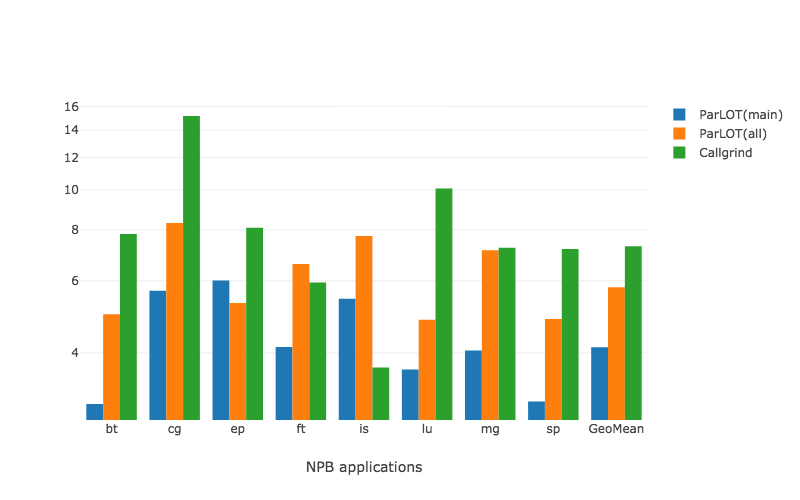
\includegraphics[width=5in]{figs.psc/chartAvg_sd_B_p3_5.png}
\caption{ Slowdown of ParLOT(main,all) and Callgrind. Each bar is the average slowdown of each tool on each application for 1, 4 and 16 nodes (16, 64 and 256 cores). Last group of bars is GeoMean (from bold numbers in table \ref{sd_pMpAcg_B_itn_p3.5}). 
}
\label{chartAvg_sd_B_p3_5}
\end{figure*}

\begin{table*}[]
\caption{Stat: sd 
 Tools: pinMain , pinAll , callgrind ,  
 Inputs: B ,  
 Nodes: 1 , 4 , 16 ,  
 Desc: Primary}
\label{ls5_sd_pMpAcg_B_itn_p3.5}\begin{center}
\begin{tabular}{lrrrrrrrrr}
\hline
                &   bt &   cg &   ep &   ft &   is &   lu &   mg &   sp &   GM \\
\hline
 pinMain.B.1    & 1.67 & 1.48 & 3.40 & 1.93 & 1.93 & 1.10 & 2.08 & 1.04 & 1.71 \\
 pinMain.B.4    & 1.63 & 1.57 & 1.69 & 2.41 & 2.33 & 1.48 & 1.53 & 3.87 & 1.95 \\
 pinMain.B.16   & 2.23 & 1.65 & 2.08 & 1.82 & 2.66 & 1.84 & 1.57 & 1.60 & 1.90 \\
 AVG            & 1.84 & 1.57 & 2.39 & 2.05 & 2.31 & 1.47 & 1.73 & 2.17 & 1.85 \\
 pinAll.B.1     & 1.97 & 2.55 & 4.15 & 2.73 & 3.71 & 1.55 & 3.96 & 1.31 & 2.53 \\
 pinAll.B.4     & 2.33 & 2.68 & 2.84 & 4.03 & 4.59 & 2.41 & 2.89 & 3.47 & 3.07 \\
 pinAll.B.16    & 4.20 & 2.68 & 4.85 & 2.71 & 8.53 & 3.34 & 2.81 & 2.98 & 3.70 \\
 AVG            & 2.83 & 2.64 & 3.95 & 3.16 & 5.61 & 2.43 & 3.22 & 2.59 & 3.10 \\
 callgrind.B.1  & 0.00 & 0.00 & 0.00 & 0.00 & 0.00 & 0.00 & 0.00 & 0.00 & 0.00 \\
 callgrind.B.4  & 0.00 & 0.00 & 0.00 & 0.00 & 0.00 & 0.00 & 0.00 & 0.00 & 0.00 \\
 callgrind.B.16 & 0.00 & 0.00 & 0.00 & 0.00 & 0.00 & 0.00 & 0.00 & 0.00 & 0.00 \\
 AVG            & 0.00 & 0.00 & 0.00 & 0.00 & 0.00 & 0.00 & 0.00 & 0.00 & 0.00 \\
\hline
\end{tabular}
\end{center}
\end{table*}


\begin{table*}[]
%\caption{Stat: sd 
 %Tools: pinMain , pinAll ,  
 %Inputs: B , C ,  
 %Nodes: 1 , 4 , 16 , 64 ,  
 % Desc: Primary}
 
 \caption{The purpose of this table is to show that ParLOT is doing better job on larger input sizes. NAS benchmark input sizes are as follows : $size(A) < size(B) < size (C) < size(D) $. The overhead it adds to the application is smaller for input size C and I believe the reason is the redundant captured data (function calls) for each run helps the performance of compressing process, thus helps the overall performance. I can run these experiments with smaller input size (A) or larger (D) and include them in this table. Running NAS applications with \textit{A} makes running times so small (less than a second for some of applications) and running with \textit{D} is going to consume a lot of SUs, if we decide to do that. Also these are the results when I use the latest version of \textit{Pin} which is \textbf{3.5}. Table \ref{sd_pMpA_BC_tni_p3.0} (next one) is identical to this table but using version \textbf{3.0} of \textit{Pin}}
 \label{sd_pMpA_BC_tni_p3.5}
\begin{center}
\begin{tabular}{|l|rrrrrrrr|r|}
\hline
              &   bt &    cg &   ep &    ft &    is &   lu &   mg &   sp &   GM \\
\hline
 pinMain.B.1  & 1.60 &  1.81 & 3.93 &  1.53 &  3.05 & 1.21 & 3.61 & 1.53 & 2.08 \\
 pinMain.C.1  & 1.39 &  1.26 & 3.12 &  1.22 &  1.95 & 1.07 & 1.49 & 1.21 & 1.50 \\
\hline
 pinMain.B.4  & 1.67 &  3.78 & 2.43 &  2.91 &  4.04 & 2.83 & 3.54 & 2.93 & 2.92 \\
 pinMain.C.4  & 1.79 &  2.79 & 3.22 &  1.78 &  3.35 & 1.38 & 2.93 & 1.63 & 2.24 \\
\hline
 pinMain.B.16 & 3.68 &  7.80 & 9.90 &  5.45 &  4.41 & 3.81 & 3.51 & 2.41 & 4.65 \\
 pinMain.C.16 & 2.88 &  4.38 & 4.38 &  3.53 &  5.14 & 3.24 & 3.50 & 2.17 & 3.54 \\
\hline
 pinMain.B.64 & 5.07 &  9.31 & 7.78 &  6.67 & 10.19 & 6.73 & 5.56 & 5.30 & 6.87 \\
 pinMain.C.64 & 5.08 &  8.56 & 6.61 &  7.35 &  7.44 & 5.21 & 3.94 & 3.81 & 5.77 \\
\hline
 pinAll.B.1   & 2.01 &  3.03 & 4.63 &  2.43 &  6.86 & 1.66 & 9.10 & 1.56 & 3.20 \\
 pinAll.C.1   & 1.49 &  1.56 & 3.72 &  1.41 &  3.25 & 1.22 & 2.65 & 1.16 & 1.87 \\
\hline
 pinAll.B.4   & 3.95 &  8.96 & 3.52 &  7.67 & 10.25 & 5.83 & 6.18 & 3.70 & 5.81 \\
 pinAll.C.4   & 2.27 &  3.42 & 4.08 &  2.52 &  5.00 & 2.15 & 4.78 & 1.83 & 3.05 \\
\hline
 pinAll.B.16  & 6.55 & 12.53 & 6.47 & 10.40 &  5.45 & 4.01 & 6.35 & 4.73 & 6.61 \\
 pinAll.C.16  & 4.89 &  3.75 & 5.48 &  4.38 &  6.21 & 3.82 & 5.04 & 2.56 & 4.38 \\
\hline
 pinAll.B.64  & 7.38 &  8.72 & 6.58 &  5.88 &  8.31 & 7.78 & 6.88 & 9.37 & 7.53 \\
 pinAll.C.64  & 7.37 &  7.30 & 5.77 &  6.38 &  6.40 & 4.80 & 4.53 & 5.19 & 5.88 \\
\hline
\end{tabular}
\end{center}
\end{table*}

\begin{table*}[]
%\caption{Stat: sd 
% Tools: pinMain , pinAll ,  
% Inputs: B , C ,  
% Nodes: 1 , 4 , 16 , 64 ,  
% Desc: Primary}

\caption{This table is similar to previous one (table \ref{sd_pMpA_BC_tni_p3.5}) but with version \textbf{3.0} of Pin. There are some zeros in the table which shows those experiments have crashed (probably because of incompatiblity of Pin with current configuration on PSC nodes). Also some of the slowdowns are smaller than 1. Thus the values of this table are not accurate and probably invalid (at least for larger number of cores). But I just wanted to include them here, in the first draft of paper, to show some differences between Pin versions and in case you are wondering why the numbers that I had in October was much better than these numbers (tables that came previously), the reason is Pin versions.}
\label{sd_pMpA_BC_tni_p3.0}
\begin{center}
\begin{tabular}{|l|rrrrrrrr|r|}
\hline
              &   bt &   cg &   ep &   ft &   is &   lu &   mg &   sp &   GM \\
\hline
 pinMain.B.1  & 1.54 & 1.81 & 3.92 & 1.71 & 4.74 & 1.37 & 3.88 & 1.47 & 2.26 \\
 pinMain.C.1  & 1.40 & 1.25 & 3.60 & 1.30 & 2.98 & 1.24 & 1.64 & 1.27 & 1.68 \\
 \hline
 pinMain.B.4  & 2.59 & 3.58 & 3.76 & 2.71 & 4.62 & 2.20 & 7.22 & 2.57 & 3.40 \\
 pinMain.C.4  & 1.66 & 2.70 & 3.59 & 1.82 & 3.01 & 1.57 & 2.82 & 1.61 & 2.24 \\
 \hline
 pinMain.B.16 & 3.57 & 4.71 & 3.79 & 4.48 & 3.77 & 3.18 & 1.91 & 2.25 & 3.32 \\
 pinMain.C.16 & 0.95 & 3.30 & 6.55 & 1.88 & 1.96 & 3.09 & 3.75 & 0.00 & 0.00 \\
 \hline
 pinMain.B.64 & 5.39 & 3.04 & 2.42 & 3.65 & 0.00 & 3.01 & 2.83 & 1.48 & 0.00 \\
 pinMain.C.64 & 1.91 & 6.75 & 1.82 & 5.03 & 4.21 & 1.56 & 6.91 & 0.89 & 2.88 \\
 \hline
 pinAll.B.1   & 1.69 & 2.31 & 5.00 & 1.99 & 5.96 & 1.54 & 5.57 & 1.57 & 2.73 \\
 pinAll.C.1   & 1.43 & 0.52 & 4.42 & 1.39 & 3.34 & 1.30 & 1.97 & 1.30 & 1.63 \\
 \hline
 pinAll.B.4   & 1.69 & 3.89 & 4.36 & 5.15 & 4.40 & 2.97 & 5.25 & 3.54 & 3.71 \\
 pinAll.C.4   & 2.09 & 2.48 & 4.32 & 1.99 & 3.46 & 1.89 & 3.35 & 0.45 & 2.14 \\
 \hline
 pinAll.B.16  & 4.48 & 5.09 & 7.41 & 2.96 & 4.70 & 5.13 & 2.67 & 3.45 & 4.27 \\
 pinAll.C.16  & 2.71 & 6.39 & 6.02 & 2.66 & 8.30 & 3.89 & 3.22 & 3.53 & 4.23 \\
 \hline
 pinAll.B.64  & 9.06 & 2.65 & 2.81 & 0.68 & 3.08 & 2.88 & 3.22 & 4.20 & 2.93 \\
 pinAll.C.64  & 6.57 & 0.00 & 4.65 & 1.74 & 2.38 & 2.56 & 0.00 & 3.66 & 0.00 \\
\hline
\end{tabular}
\end{center}
\end{table*}

\begin{table*}[]
\caption{Stat: sd 
 Tools: pinMain , pinAll ,  
 Inputs: B , C ,  
 Nodes: 1 , 4 , 16 , 64 ,  
 Desc: Primary}
\label{ls5_sd_pMpA_BC_tni_p3.5}\begin{center}
\begin{tabular}{lrrrrrrrrr}
\hline
              &   bt &   cg &   ep &   ft &   is &   lu &   mg &   sp &   GM \\
\hline
 pinMain.B.1  & 1.67 & 1.48 & 3.40 & 1.93 & 1.93 & 1.10 & 2.08 & 1.04 & 1.71 \\
 pinMain.C.1  & 2.52 & 1.05 & 4.63 & 1.98 & 1.57 & 0.62 & 1.96 & 1.06 & 1.63 \\
 AVG          & 2.09 & 1.27 & 4.01 & 1.96 & 1.75 & 0.86 & 2.02 & 1.05 & 1.67 \\
 pinMain.B.4  & 1.63 & 1.57 & 1.69 & 2.41 & 2.33 & 1.48 & 1.53 & 3.87 & 1.95 \\
 pinMain.C.4  & 2.78 & 1.49 & 4.19 & 1.99 & 2.68 & 1.32 & 3.43 & 0.91 & 2.10 \\
 AVG          & 2.21 & 1.53 & 2.94 & 2.20 & 2.50 & 1.40 & 2.48 & 2.39 & 2.02 \\
 pinMain.B.16 & 2.23 & 1.65 & 2.08 & 1.82 & 2.66 & 1.84 & 1.57 & 1.60 & 1.90 \\
 pinMain.C.16 & 2.00 & 2.84 & 5.19 & 1.32 & 4.07 & 2.45 & 3.05 & 1.80 & 2.61 \\
 AVG          & 2.12 & 2.25 & 3.64 & 1.57 & 3.37 & 2.15 & 2.31 & 1.70 & 2.25 \\
 pinMain.B.64 & 2.59 & 2.64 & 2.04 & 2.59 & 2.38 & 2.69 & 2.41 & 2.82 & 2.51 \\
 pinMain.C.64 & 2.39 & 2.80 & 2.41 & 2.18 & 2.48 & 2.48 & 2.75 & 2.39 & 2.48 \\
 AVG          & 2.49 & 2.72 & 2.23 & 2.38 & 2.43 & 2.58 & 2.58 & 2.60 & 2.50 \\
 pinAll.B.1   & 1.97 & 2.55 & 4.15 & 2.73 & 3.71 & 1.55 & 3.96 & 1.31 & 2.53 \\
 pinAll.C.1   & 1.42 & 1.28 & 3.32 & 2.21 & 2.87 & 0.64 & 2.59 & 1.66 & 1.79 \\
 AVG          & 1.69 & 1.92 & 3.74 & 2.47 & 3.29 & 1.09 & 3.27 & 1.48 & 2.16 \\
 pinAll.B.4   & 2.33 & 2.68 & 2.84 & 4.03 & 4.59 & 2.41 & 2.89 & 3.47 & 3.07 \\
 pinAll.C.4   & 3.40 & 3.75 & 8.72 & 5.22 & 7.27 & 1.68 & 3.29 & 1.18 & 3.59 \\
 AVG          & 2.87 & 3.21 & 5.78 & 4.62 & 5.93 & 2.04 & 3.09 & 2.33 & 3.33 \\
 pinAll.B.16  & 4.20 & 2.68 & 4.85 & 2.71 & 8.53 & 3.34 & 2.81 & 2.98 & 3.70 \\
 pinAll.C.16  & 2.90 & 2.58 & 5.04 & 2.18 & 4.49 & 4.73 & 5.45 & 2.13 & 3.45 \\
 AVG          & 3.55 & 2.63 & 4.95 & 2.45 & 6.51 & 4.04 & 4.13 & 2.55 & 3.58 \\
 pinAll.B.64  & 5.28 & 4.91 & 4.01 & 5.02 & 4.37 & 6.09 & 4.82 & 6.31 & 5.05 \\
 pinAll.C.64  & 4.68 & 4.83 & 4.68 & 4.73 & 4.82 & 5.65 & 4.97 & 4.73 & 4.88 \\
 AVG          & 4.98 & 4.87 & 4.34 & 4.88 & 4.60 & 5.87 & 4.89 & 5.52 & 4.96 \\
\hline
\end{tabular}
\end{center}
\end{table*}



\begin{table*}[]
%\caption{Stat: bw 
% Tools: pinMain , pinAll , callgrind ,  
% Inputs: B ,  
% Nodes: 1 , 4 , 16 ,  
% Desc: Primary}


\caption{This table is showing the required bandwidth for each application (KiloBytes per core per second). $ReqBW_x = TraceSize_x (KB) / (\# of cores)_x / Runtime_x (S)$
Because of the crashing problems of Callgrind on \textit{C} input and 64 nodes, I only include \textit{B} input and 1, 4, and 16 nodes results. Clearly ParLOT(main) is beating Callgrind while they both generate the same information (I still believe ParLOT(main) generated traces are more informative and rich). ParLOT(all) bandwidth is the highest but with capturing all of the function calls within a single execution, there is no surprise. Another interesting fact from this table is, for ParLOT(main), bandwidth drops from \textbf{0.62} for 16 cores to \textbf{0.27} for 256 cores (good scalability). It is the opposite for Callgrind where the required bandwidth jumps from \textbf{3.28} (KB/s) for 16 cores to \textbf{33.06} (KB/S) for 256 cores. I also have the results of required bandwidth of ParLOT for 64 nodes(1024 cores) and Input C but I did not include them here because I did not have them for Callgrind (explained above).  Fig \ref{chartAvg_bw_B_p3_5} visualize these numbers (Average values)}
\label{bw_pMpAcg_B_itn_p3.5}
\begin{center}
\begin{tabular}{|l|rrrrrrrr|r|}
\hline
                &    bt &    cg &    ep &    ft &    is &    lu &    mg &    sp &    GM \\
\hline
 pinMain.B.1    &  2.54 & 22.73 &  0.99 &  0.33 &  0.46 &  0.10 &  0.43 &  0.06 &  0.62 \\
 pinMain.B.4    &  3.20 & 18.31 &  0.52 &  0.20 &  0.12 &  0.11 &  0.23 &  0.10 &  0.46 \\
 pinMain.B.16   &  2.20 &  9.66 &  0.09 &  0.14 &  0.06 &  0.08 &  0.19 &  0.13 &  0.27 \\
 \hline
 AVG            &  2.65 & 16.90 &  0.53 &  0.22 &  0.21 &  0.10 &  0.28 &  0.10 &  \textbf{0.45} \\
 \hline
 pinAll.B.1     & 20.80 & 39.89 & 14.75 & 21.05 & 31.00 & 19.55 & 34.37 & 12.37 & 22.53 \\
 pinAll.B.4     & 21.85 & 33.10 & 22.15 & 17.05 & 16.19 & 35.84 & 34.53 & 35.99 & 25.81 \\
 pinAll.B.16    & 25.31 & 29.33 & 23.31 & 20.07 & 23.78 & 56.58 & 29.09 & 42.96 & 29.57 \\
 \hline
 AVG            & 22.65 & 34.11 & 20.07 & 19.39 & 23.66 & 37.32 & 32.66 & 30.44 & \textbf{25.97} \\
 \hline
 callgrind.B.1  &  0.90 &  2.40 &  2.53 &  4.02 & 24.33 &  1.39 & 14.64 &  1.22 &  3.28 \\
 callgrind.B.4  &  4.27 &  9.11 & 12.02 & 16.78 & 59.03 &  2.97 & 35.78 &  5.20 & 11.25 \\
 callgrind.B.16 & 17.48 & 12.87 & 46.08 & 51.94 & 87.05 & 19.13 & 48.00 & 33.18 & 33.06 \\
 \hline
 AVG            &  7.55 &  8.13 & 20.21 & 24.25 & 56.80 &  7.83 & 32.81 & 13.20 & \textbf{15.86} \\
\hline
\end{tabular}
\end{center}
\end{table*}


\begin{figure*}[!t]
\centering
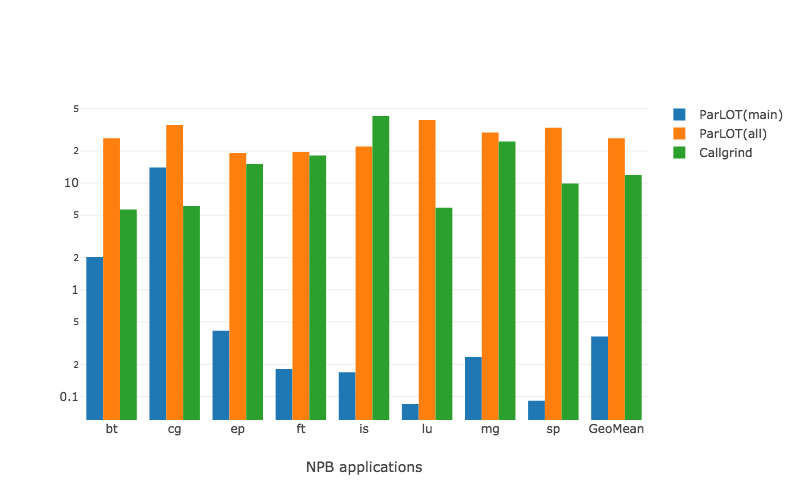
\includegraphics[width=5in]{figs.psc/chartAvg_bw_B_p3_5.png}
\caption{ Required Bandwidth (KB) per core per second for ParLOT and Callgrind.  
(Input: B)}
\label{chartAvg_bw_B_p3_5}
\end{figure*}


\begin{table*}[]
\caption{Similar to previous table (table \ref{bw_pMpAcg_B_itn_p3.5}) for all number of nodes for \textbf{C} input}
\label{bw_pMpA_C_itn_p3.5}\begin{center}
\begin{tabular}{|l|rrrrrrrr|r|}
\hline
              &    bt &    cg &    ep &    ft &    is &    lu &    mg &    sp &    GM \\
\hline
 pinMain.C.1  &  1.08 & 13.81 &  1.26 &  0.13 &  0.66 &  0.03 &  0.20 &  0.02 &  0.34 \\
 pinMain.C.4  &  1.49 & 26.18 &  0.92 &  0.15 &  0.18 &  0.07 &  0.19 &  0.05 &  0.40 \\
 pinMain.C.16 &  2.81 & 18.28 &  0.41 &  0.13 &  0.08 &  0.08 &  0.14 &  0.07 &  0.34 \\
 pinMain.C.64 &  1.69 & 10.24 &  0.09 &  0.06 &  0.03 &  0.04 &  0.09 &  0.06 &  0.17 \\
 \hline
 AVG          &  1.77 & 17.13 &  0.67 &  0.12 &  0.24 &  0.06 &  0.15 &  0.05 &  \textbf{0.31} \\
 \hline
 pinAll.C.1   &  7.42 & 22.04 &  6.47 &  9.30 & 22.51 &  8.11 & 20.92 &  3.73 & 10.43 \\
 pinAll.C.4   & 20.76 & 60.33 & 13.91 & 23.08 & 28.33 & 36.31 & 30.00 & 20.85 & 26.71 \\
 pinAll.C.16  & 26.08 & 65.31 & 20.39 & 29.43 & 26.92 & 71.97 & 28.06 & 41.71 & 35.13 \\
 pinAll.C.64  & 31.06 & 47.34 & 17.55 & 20.57 & 21.77 & 61.31 & 23.31 & 42.41 & 30.25 \\
 \hline
 AVG          & 21.33 & 48.76 & 14.58 & 20.59 & 24.88 & 44.42 & 25.57 & 27.18 & \textbf{25.63} \\
\hline
\end{tabular}
\end{center}
\end{table*}

%\begin{table}[]
\caption{Stat: bw 
 Tools: pinMain , pinAll , callgrind ,  
 Inputs: B ,  
 Nodes: 1 , 4 , 16 ,  
 Desc: Primary}
\begin{center}
\begin{tabular}{|l|rrrrrrrr|r|}
\hline
                &    bt &    cg &    ep &    ft &    is &    lu &    mg &    sp &    GM \\
\hline
 pinMain.B.1    &  2.54 & 22.73 &  0.99 &  0.33 &  0.46 &   0.1 &  0.43 &  0.06 &  0.62 \\
 pinAll.B.1     &  20.8 & 39.89 & 14.75 & 21.05 &    31 & 19.55 & 34.37 & 12.37 & 22.53 \\
 callgrind.B.1  &   0.9 &   2.4 &  2.53 &  4.02 & 24.33 &  1.39 & 14.64 &  1.22 &  3.28 \\
\hline
 pinMain.B.4    &   3.2 & 18.31 &  0.52 &   0.2 &  0.12 &  0.11 &  0.23 &   0.1 &  0.46 \\
 pinAll.B.4     & 21.85 &  33.1 & 22.15 & 17.05 & 16.19 & 35.84 & 34.53 & 35.99 & 25.81 \\
 callgrind.B.4  &  4.27 &  9.11 & 12.02 & 16.78 & 59.03 &  2.97 & 35.78 &   5.2 & 11.25 \\
 \hline
 pinMain.B.16   &   2.2 &  9.66 &  0.09 &  0.14 &  0.06 &  0.08 &  0.19 &  0.13 &  0.27 \\
 pinAll.B.16    & 25.31 & 29.33 & 23.31 & 20.07 & 23.78 & 56.58 & 29.09 & 42.96 & 29.57 \\
 callgrind.B.16 & 17.48 & 12.87 & 46.08 & 51.94 & 87.05 & 19.13 &    48 & 33.18 & 33.06 \\

\hline
\end{tabular}
\end{center}
\end{table}



\begin{table*}[]
%\caption{Stat: cr 
% Tools: pinMain , pinAll ,  
% Inputs: C , B ,  
% Nodes: 1 , 4 , 16 , 64 ,  
% Desc: Primary}
\caption{COMPRESSION RATIOS FOR B AND C INPUTS AND 1, 4, 16 AND 64 NODES.}
\label{cr_pMpA_BC_itn_p3.5}
\begin{center}
\begin{tabular}{|l|rrrrrrrr|r|}
\hline
              &       bt &      cg &       ep &       ft &       is &       lu &      mg &       sp &      GM \\
\hline
 pinMain.C.1  & 14051.90 &   85.18 & 12104.15 & 31406.62 & 36422.85 & 20423.90 & 1169.56 & 22561.69 & 7393.79 \\
 pinMain.C.4  &  8249.54 &   85.36 & 12067.24 & 24222.90 & 33655.89 & 11191.63 &  650.18 & 10441.99 & 5189.93 \\
 pinMain.C.16 &  1985.31 &   85.55 & 11921.80 & 11426.88 & 25812.61 &  7353.92 &  353.38 &  4810.38 & 3048.85 \\
 pinMain.C.64 &   709.30 &   85.74 & 11374.25 &  6738.89 & 13360.80 &  6916.77 &  250.95 &  4624.28 & 2174.51 \\
 \hline
 AVG          &  6249.01 &   85.46 & 11866.86 & 18448.82 & 27313.04 & 11471.56 &  606.02 & 10609.58 & 4451.77 \\
 \hline
 pinAll.C.1   &  2579.37 &   89.08 & 21213.12 &  6818.31 &  7698.78 &   135.16 &   89.48 &   272.48 &  978.90 \\
 pinAll.C.4   &  1441.93 &  301.17 & 13242.06 &  1412.63 &  1122.81 &   709.17 &  857.56 &   773.11 & 1199.60 \\
 pinAll.C.16  &  1954.84 &  413.29 &  6721.88 &  1531.17 &  1793.81 &   430.15 & 1317.55 &   820.22 & 1273.86 \\
 pinAll.C.64  &  1195.58 &  891.83 &  5537.37 &  3191.36 &  2461.46 &   676.34 & 2412.46 &   967.72 & 1710.36 \\
 \hline
 AVG          &  1792.93 &  423.84 & 11678.61 &  3238.37 &  3269.22 &   487.71 & 1169.26 &   708.38 & 1290.68 \\
 \hline
 pinMain.B.1  &  5403.04 &   74.95 & 12067.06 & 12704.90 & 33655.87 &  8750.65 &  541.98 & 10426.05 & 4234.22 \\
 pinMain.B.4  &  2129.01 &   75.33 & 11922.18 & 10745.40 & 25812.57 &  5128.06 &  364.22 &  4042.15 & 2820.40 \\
 pinMain.B.16 &   729.64 &   75.70 & 11374.86 &  3508.41 & 13360.75 &  4371.76 &  205.67 &  3265.36 & 1746.25 \\
 pinMain.B.64 &  3551.97 &   76.08 &  9608.18 &  2790.59 &  4563.29 &  4031.59 &  164.19 &  4030.09 & 1750.60 \\
 \hline
 AVG          &  2953.41 &   75.52 & 11243.07 &  7437.32 & 19348.12 &  5570.52 &  319.02 &  5440.91 & 2637.87 \\
 \hline
 pinAll.B.1   &   750.27 &   68.40 & 16927.14 &  2584.15 &  2304.36 &   101.34 &   69.80 &   119.94 &  507.33 \\
 pinAll.B.4   &  1693.37 &  649.30 &  6797.11 &  2165.42 &  2402.91 &   727.52 &  836.96 &   672.73 & 1413.43 \\
 pinAll.B.16  &  1265.26 & 1138.20 &  4140.31 &  1794.78 &  1993.44 &   620.41 & 1477.61 &   883.86 & 1427.94 \\
 pinAll.B.64  &  1294.03 & 1218.33 &  5187.85 &  3086.80 &  3266.69 &  1044.65 & 2520.99 &  1167.23 & 1997.57 \\
 \hline
 AVG          &  1250.73 &  768.56 &  8263.10 &  2407.79 &  2491.85 &   623.48 & 1226.34 &   710.94 & 1336.57 \\

\hline
\end{tabular}
\end{center}
\end{table*}


%\begin{table*}[]
\caption{Stat: cr 
 Tools: pinMain , pinAll ,  
 Inputs: B , C ,  
 Nodes: 1 , 4 , 16 , 64 ,  
 Desc: Primary}
\begin{center}
\begin{tabular}{lrrrrrrrrr}
\hline
              &      bt &      cg &      ep &      ft &      is &      lu &      mg &      sp &      GM \\
\hline
 pinMain.B.1  & 5403.04 &   74.95 & 12067.1 & 12704.9 & 33655.9 & 8750.65 &  541.98 &   10426 & 4234.22 \\
 pinAll.B.1   &  750.27 &    68.4 & 16927.1 & 2584.15 & 2304.36 &  101.34 &    69.8 &  119.94 &  507.33 \\
 AVG          & 3076.65 &   71.68 & 14497.1 & 7644.52 & 17980.1 & 4425.99 &  305.89 & 5272.99 & 2370.78 \\
 pinMain.B.4  & 2129.01 &   75.33 & 11922.2 & 10745.4 & 25812.6 & 5128.06 &  364.22 & 4042.15 &  2820.4 \\
 pinAll.B.4   & 1693.37 &   649.3 & 6797.11 & 2165.42 & 2402.91 &  727.52 &  836.96 &  672.73 & 1413.43 \\
 AVG          & 1911.19 &  362.31 & 9359.65 & 6455.41 & 14107.7 & 2927.79 &  600.59 & 2357.44 & 2116.91 \\
 pinMain.B.16 &  729.64 &    75.7 & 11374.9 & 3508.41 & 13360.8 & 4371.76 &  205.67 & 3265.36 & 1746.25 \\
 pinAll.B.16  & 1265.26 &  1138.2 & 4140.31 & 1794.78 & 1993.44 &  620.41 & 1477.61 &  883.86 & 1427.94 \\
 AVG          &  997.45 &  606.95 & 7757.59 & 2651.59 &  7677.1 & 2496.09 &  841.64 & 2074.61 &  1587.1 \\
 pinMain.B.64 & 3551.97 &   76.08 & 9608.18 & 2790.59 & 4563.29 & 4031.59 &  164.19 & 4030.09 &  1750.6 \\
 pinAll.B.64  & 1294.03 & 1218.33 & 5187.85 &  3086.8 & 3266.69 & 1044.65 & 2520.99 & 1167.23 & 1997.57 \\
 AVG          &    2423 &   647.2 & 7398.02 &  2938.7 & 3914.99 & 2538.12 & 1342.59 & 2598.66 & 1874.09 \\
 pinMain.C.1  & 14051.9 &   85.18 & 12104.1 & 31406.6 & 36422.8 & 20423.9 & 1169.56 & 22561.7 & 7393.79 \\
 pinAll.C.1   & 2579.37 &   89.08 & 21213.1 & 6818.31 & 7698.78 &  135.16 &   89.48 &  272.48 &   978.9 \\
 AVG          & 8315.64 &   87.13 & 16658.6 & 19112.5 & 22060.8 & 10279.5 &  629.52 & 11417.1 & 4186.35 \\
 pinMain.C.4  & 8249.54 &   85.36 & 12067.2 & 24222.9 & 33655.9 & 11191.6 &  650.18 &   10442 & 5189.93 \\
 pinAll.C.4   & 1441.93 &  301.17 & 13242.1 & 1412.63 & 1122.81 &  709.17 &  857.56 &  773.11 &  1199.6 \\
 AVG          & 4845.74 &  193.27 & 12654.6 & 12817.8 & 17389.3 &  5950.4 &  753.87 & 5607.55 & 3194.77 \\
 pinMain.C.16 & 1985.31 &   85.55 & 11921.8 & 11426.9 & 25812.6 & 7353.92 &  353.38 & 4810.38 & 3048.85 \\
 pinAll.C.16  & 1954.84 &  413.29 & 6721.88 & 1531.17 & 1793.81 &  430.15 & 1317.55 &  820.22 & 1273.86 \\
 AVG          & 1970.07 &  249.42 & 9321.84 & 6479.02 & 13803.2 & 3892.03 &  835.46 &  2815.3 & 2161.36 \\
 pinMain.C.64 &   709.3 &   85.74 & 11374.2 & 6738.89 & 13360.8 & 6916.77 &  250.95 & 4624.28 & 2174.51 \\
 pinAll.C.64  & 1195.58 &  891.83 & 5537.37 & 3191.36 & 2461.46 &  676.34 & 2412.46 &  967.72 & 1710.36 \\
 AVG          &  952.44 &  488.79 & 8455.81 & 4965.12 & 7911.13 & 3796.56 &  1331.7 &    2796 & 1942.43 \\
\hline
\end{tabular}
\end{center}
\end{table*}


\begin{table*}[]
%\caption{Stat: sd 
% Tools:  
% Inputs: B ,  
% Nodes: 1 , 4 , 16 , 64 ,  
% Desc: Detail Report}

\caption{Server: \textbf{PSC} - Tables \ref{det_Main_all_B_p3.5}, \ref{comet_det_Main_all_B_p3.5}, \ref{ls5_det_Main_all_B_p3.5}, \ref{det_All_all_B_p3.5}, \ref{comet_det_All_all_B_p3.5} and \ref{ls5_det_All_all_B_p3.5}  are showing the detail slowdowns added to the code by each phase of ParLOT(main and all) for input size \textit{B} on \textbf{PSC}, \textbf{Comet} and \textbf{Lonestar5}. I put my observations of all four tables over here. \textbf{npin} is just the slowdown caused by initializing Pin's routines on top of the target application without doing anything else (no instrumentation, tracing, compression and I/O.  \textbf{dpin} is almost identical to ParLOT except it stores the generated compressed traces to "/dev/null". The purpose of \textit{dpin} is to see how much of the overall overhead is because of I/O and data-related slowdowns. In \textbf{wpin}, and all collected data would be stored as is to the disk. The results of this tools shows how much efficiency our compression approach adds to ParLOT. Last row of tables shows geometric mean of each of its above values showing how much each phase of ParLOT slows down the native execution. In general, we all expect that the slowdowns of $npin < dpin < ParLOT < wpin $. But majority of numbers are not like that. I double checked the results of CHPC and Stampede and the patterns are kind of identical.  In most of the table entries (in particular for smaller number of cores), the differences between the average slowdown of \textit{dpin} and \textit{ParLOT} is very insignificant which shows that ParLOT is not an I/O-bounded tool. Figures \ref{chartDet_B_wc_byTool_p3_5} and \ref{chartDet_B_woc_byTool_p3_5} visualize numbers from these tables.} 
\label{det_Main_all_B_p3.5}

\begin{center}
\scalebox{0.95}{
\begin{tabular}{|c|c|rrrr|rrrr|rrrr|rrrr|} 
\hline 
\multicolumn{1}{|l|}{\multirow{2}{*}{\textbf{Input: B}}} & \multicolumn{1}{r|}{Nodes :}    & \multicolumn{4}{c|}{1}  & \multicolumn{4}{c|}{4} & \multicolumn{4}{c|}{16}  & \multicolumn{4}{c|}{64} \\ \cline{2-18} 
\multicolumn{1}{|l|}{} & \multicolumn{1}{r|}{Detail Tools:} & \multicolumn{1}{c}{npin} & \multicolumn{1}{c}{dpin} & \multicolumn{1}{c}{ParLOT} & \multicolumn{1}{c|}{wpin} & \multicolumn{1}{c}{npin} & \multicolumn{1}{c}{dpin} & \multicolumn{1}{c}{ParLOT} & \multicolumn{1}{c|}{wpin} & \multicolumn{1}{c}{npin} & \multicolumn{1}{c}{dpin} & \multicolumn{1}{c}{ParLOT} & \multicolumn{1}{c|}{wpin} & \multicolumn{1}{c}{npin} & \multicolumn{1}{c}{dpin} & \multicolumn{1}{c}{ParLOT} & \multicolumn{1}{c|}{wpin} \\
\hline
\multirow{9}{*}{Main} &  bt  &  1.49  &  1.52  &  1.60  &  11.63  &  1.17  &  1.58  &  1.67  &  8.53  &  1.86  &  2.99  &  3.68  &   8.81  &  4.22  &  4.51  &   5.07  &  13.64 \\
 &  cg  &  1.78  & \cellcolor{blue!25} 1.76  &  1.81  &   3.19  &  2.64  &  5.02  & \cellcolor{blue!25} 3.78  &  6.76  &  4.86  &  6.27  &  7.80  &  12.38  &  3.92  &  8.43  &   9.31  &  12.96 \\
 &  ep  &  3.82  & \cellcolor{blue!25} 3.37  &  3.93  &  22.47  &  1.84  &  2.26  &  2.43  &  7.94  &  4.97  &  5.02  &  9.90  & \cellcolor{blue!25}  9.09  &  3.27  &  7.22  &   7.78  &   7.67 \\
 &  ft  &  1.60  & \cellcolor{blue!25} 1.51  &  1.53  &   3.23  &  2.43  &  4.36  & \cellcolor{blue!25} 2.91  &  4.31  &  3.52  &  5.90  & \cellcolor{blue!25} 5.45  &   5.87  &  3.24  &  6.87  & \cellcolor{blue!25}  6.67  &   6.69 \\
 &  is  &  3.61  & \cellcolor{blue!25} 3.55  & \cellcolor{blue!25} 3.05  &  14.60  &  3.20  &  3.68  &  4.04  &  5.88  &  3.85  &  4.82  & \cellcolor{blue!25} 4.41  &   4.67  &  4.80  &  9.99  &  10.19  &  10.46 \\
 &  lu  &  1.39  & \cellcolor{blue!25} 1.20  &  1.21  &   1.58  &  1.85  &  2.07  &  2.83  &  3.52  &  1.64  &  3.00  &  3.81  &   5.53  &  3.17  &  6.77  & \cellcolor{blue!25}  6.73  &  13.70 \\
 &  mg  &  3.91  & \cellcolor{blue!25} 3.51  &  3.61  &   3.84  &  3.19  &  3.34  &  3.54  &  3.96  &  2.95  &  3.36  &  3.51  &   3.82  &  3.70  &  5.57  & \cellcolor{blue!25}  5.56  &   5.70 \\
 &  sp  &  1.25  &  1.43  &  1.53  &   1.65  &  2.13  &  4.38  & \cellcolor{blue!25} 2.93  &  3.63  &  2.98  &  3.48  & \cellcolor{blue!25} 2.41  &   3.86  &  4.28  &  5.78  & \cellcolor{blue!25}  5.30  &   8.56 \\ \cline{2-18}
 &  GM  &  2.11  & \cellcolor{blue!25} 2.03  &  2.08  &   5.00  &  2.20  &  3.11  & \cellcolor{blue!25} 2.92  &  5.26  &  3.11  &  4.18  &  4.65  &   6.21  &  3.79  &  6.71  &   6.87  &   9.45 \\
\hline 
\end{tabular} }

\end{center}
\end{table*}









\begin{table*}[]
\caption{Stat: sd 
 Tools:  
 Inputs: B ,  
 Nodes: 1 , 4 , 16 , 64 ,  
 Desc: Detail Report}
\begin{center}
\label{ls5_det_Main_all_B_p3.5}
\scalebox{0.95}{
\begin{tabular}{|c|c|rrrr|rrrr|rrrr|rrrr|} 
\hline 
\multicolumn{1}{|l|}{\multirow{2}{*}{\textbf{Input: B}}} & \multicolumn{1}{r|}{Nodes :}    & \multicolumn{4}{c|}{1}  & \multicolumn{4}{c|}{4} & \multicolumn{4}{c|}{16}  & \multicolumn{4}{c|}{64} \\ \cline{2-18} 
\multicolumn{1}{|l|}{} & \multicolumn{1}{r|}{Detail Tools:} & \multicolumn{1}{c}{npin} & \multicolumn{1}{c}{dpin} & \multicolumn{1}{c}{ParLOT} & \multicolumn{1}{c|}{wpin} & \multicolumn{1}{c}{npin} & \multicolumn{1}{c}{dpin} & \multicolumn{1}{c}{ParLOT} & \multicolumn{1}{c|}{wpin} & \multicolumn{1}{c}{npin} & \multicolumn{1}{c}{dpin} & \multicolumn{1}{c}{ParLOT} & \multicolumn{1}{c|}{wpin} & \multicolumn{1}{c}{npin} & \multicolumn{1}{c}{dpin} & \multicolumn{1}{c}{ParLOT} & \multicolumn{1}{c|}{wpin} \\
\hline
\multirow{9}{*}{Main} &  bt  &  2.11  & \cellcolor{blue!25} 1.67  &  1.67  &   6.86  &  1.24  &  1.57  &  1.63  &  9.99  &  1.25  &  2.18  &  2.23  &  6.96  &  2.38  &  2.54  &  2.59  &  3.26 \\
 &  cg  &  1.50  &  2.85  & \cellcolor{blue!25} 1.48  &   3.33  &  1.46  &  2.71  & \cellcolor{blue!25} 1.57  &  3.28  &  2.25  &  2.80  & \cellcolor{blue!25} 1.65  &  4.32  &  2.54  &  2.73  & \cellcolor{blue!25} 2.64  &  3.55 \\
 &  ep  &  3.09  &  3.92  & \cellcolor{blue!25} 3.40  &  16.33  &  1.49  &  1.63  &  1.69  &  7.96  &  1.60  &  2.24  & \cellcolor{blue!25} 2.08  &  3.75  &  2.11  &  2.28  & \cellcolor{blue!25} 2.04  &  2.69 \\
 &  ft  &  1.58  &  1.91  &  1.93  &   8.71  &  2.19  &  2.90  & \cellcolor{blue!25} 2.41  &  6.75  &  2.24  &  2.28  & \cellcolor{blue!25} 1.82  &  3.94  &  2.73  & \cellcolor{blue!25} 2.46  &  2.59  &  2.49 \\
 &  is  &  2.01  &  3.00  & \cellcolor{blue!25} 1.93  &   2.03  &  2.35  & \cellcolor{blue!25} 2.32  &  2.33  &  4.60  &  2.41  &  3.88  & \cellcolor{blue!25} 2.66  &  5.24  &  2.33  & \cellcolor{blue!25} 2.26  &  2.38  &  2.31 \\
 &  lu  &  1.16  &  1.23  & \cellcolor{blue!25} 1.10  &   1.21  &  1.71  &  2.72  & \cellcolor{blue!25} 1.48  &  2.58  &  2.50  &  2.83  & \cellcolor{blue!25} 1.84  &  3.05  &  2.61  & \cellcolor{blue!25} 2.54  &  2.69  &  3.11 \\
 &  mg  &  2.25  & \cellcolor{blue!25} 2.05  &  2.08  &   4.22  &  1.38  &  2.40  & \cellcolor{blue!25} 1.53  &  2.71  &  2.09  &  2.45  & \cellcolor{blue!25} 1.57  &  3.04  &  3.04  & \cellcolor{blue!25} 2.87  & \cellcolor{blue!25} 2.41  &  3.09 \\
 &  sp  &  0.98  &  1.80  & \cellcolor{blue!25} 1.04  &   3.26  &  1.89  &  2.11  &  3.87  &  8.24  &  2.49  &  2.49  & \cellcolor{blue!25} 1.60  &  2.81  &  2.82  & \cellcolor{blue!25} 2.58  &  2.82  &  2.82 \\
 &  GM  &  1.73  &  2.17  & \cellcolor{blue!25} 1.71  &   4.27  &  1.67  &  2.24  & \cellcolor{blue!25} 1.95  &  5.11  &  2.05  &  2.60  & \cellcolor{blue!25} 1.90  &  3.96  &  2.55  & \cellcolor{blue!25} 2.53  & \cellcolor{blue!25} 2.51  &  2.89 \\
\hline 
\end{tabular} }

\end{center}
\end{table*}


\begin{table*}[]
\caption{Input: C , Main}
 \label{det_Main_all_C_p3.5}
\begin{center}
\scalebox{0.95}{
\begin{tabular}{|c|c|rrrr|rrrr|rrrr|rrrr|} 
\hline 
\multicolumn{1}{|l|}{\multirow{2}{*}{\textbf{Input: C}}} & \multicolumn{1}{r|}{Nodes :}    & \multicolumn{4}{c|}{1}  & \multicolumn{4}{c|}{4} & \multicolumn{4}{c|}{16}  & \multicolumn{4}{c|}{64} \\ \cline{2-18} 
\multicolumn{1}{|l|}{} & \multicolumn{1}{r|}{Detail Tools:} & \multicolumn{1}{c}{npin} & \multicolumn{1}{c}{dpin} & \multicolumn{1}{c}{ParLOT} & \multicolumn{1}{c|}{wpin} & \multicolumn{1}{c}{npin} & \multicolumn{1}{c}{dpin} & \multicolumn{1}{c}{ParLOT} & \multicolumn{1}{c|}{wpin} & \multicolumn{1}{c}{npin} & \multicolumn{1}{c}{dpin} & \multicolumn{1}{c}{ParLOT} & \multicolumn{1}{c|}{wpin} & \multicolumn{1}{c}{npin} & \multicolumn{1}{c}{dpin} & \multicolumn{1}{c}{ParLOT} & \multicolumn{1}{c|}{wpin} \\
\hline
\multirow{9}{*}{Main} &  bt  &  1.35  &  1.38  &  1.39  &  0.00  &  2.21  & \cellcolor{blue!25} 1.70  &  1.79  &  0.00  &  2.18  &  2.76  &  2.88  &  0.00  &  3.61  &  4.64  &  5.08  &  0.00 \\
 &  cg  &  1.24  &  1.79  & \cellcolor{blue!25} 1.26  &  0.00  &  2.06  &  2.69  &  2.79  &  0.00  &  2.03  &  4.54  & \cellcolor{blue!25} 4.38  &  0.00  &  5.66  &  8.73  & \cellcolor{blue!25} 8.56  &  0.00 \\
 &  ep  &  3.58  & \cellcolor{blue!25} 3.36  & \cellcolor{blue!25} 3.12  &  0.00  &  2.32  &  3.16  &  3.22  &  0.00  &  3.43  &  4.26  &  4.38  &  0.00  &  4.53  &  6.86  & \cellcolor{blue!25} 6.61  &  0.00 \\
 &  ft  &  1.29  & \cellcolor{blue!25} 1.23  & \cellcolor{blue!25} 1.22  &  0.00  &  1.56  &  1.77  &  1.78  &  0.00  &  2.57  &  3.41  &  3.53  &  0.00  &  4.33  &  7.55  & \cellcolor{blue!25} 7.35  &  0.00 \\
 &  is  &  2.96  & \cellcolor{blue!25} 1.98  & \cellcolor{blue!25} 1.95  &  0.00  &  2.66  &  3.20  &  3.35  &  0.00  &  3.48  &  6.15  & \cellcolor{blue!25} 5.14  &  0.00  &  4.21  &  7.49  & \cellcolor{blue!25} 7.44  &  0.00 \\
 &  lu  &  2.56  & \cellcolor{blue!25} 1.07  &  1.07  &  0.00  &  1.29  &  1.35  &  1.38  &  0.00  &  2.97  &  3.21  &  3.24  &  0.00  &  2.81  &  5.20  &  5.21  &  0.00 \\
 &  mg  &  1.55  &  2.73  & \cellcolor{blue!25} 1.49  &  0.00  &  2.44  &  2.87  &  2.93  &  0.00  &  2.61  &  2.95  &  3.50  & 0.00  &  2.82  &  3.63  &  3.94  &  0.00 \\
 &  sp  &  1.05  &  1.21  &  1.21  &  0.00  &  1.30  &  1.63  &  1.63  &  0.00  &  1.46  &  2.57  & \cellcolor{blue!25} 2.17  &  0.00  &  2.84  &  3.39  &  3.81  &  0.00 \\ \cline{2-18}
 &  GM  &  1.77  & \cellcolor{blue!25} 1.71  & \cellcolor{blue!25} 1.50  &  0.00  &  1.91  &  2.18  &  2.24  &  0.00  &  2.50  &  3.58  & \cellcolor{blue!25} 3.54  &  0.00  &  3.74  &  5.63  &  5.77  &  0.00 \\
\hline 
\end{tabular} }

\end{center}
\end{table*}

\begin{table*}[]
\caption{Stat: sd 
 Tools:  
 Inputs: C ,  
 Nodes: 1 , 4 , 16 , 64 ,  
 Desc: Detail Report}
\begin{center}
\label{ls5_det_Main_all_C_p3.5}
\scalebox{0.95}{
\begin{tabular}{|c|c|rrrr|rrrr|rrrr|rrrr|} 
\hline 
\multicolumn{1}{|l|}{\multirow{2}{*}{\textbf{Input: C}}} & \multicolumn{1}{r|}{Nodes :}    & \multicolumn{4}{c|}{1}  & \multicolumn{4}{c|}{4} & \multicolumn{4}{c|}{16}  & \multicolumn{4}{c|}{64} \\ \cline{2-18} 
\multicolumn{1}{|l|}{} & \multicolumn{1}{r|}{Detail Tools:} & \multicolumn{1}{c}{npin} & \multicolumn{1}{c}{dpin} & \multicolumn{1}{c}{ParLOT} & \multicolumn{1}{c|}{wpin} & \multicolumn{1}{c}{npin} & \multicolumn{1}{c}{dpin} & \multicolumn{1}{c}{ParLOT} & \multicolumn{1}{c|}{wpin} & \multicolumn{1}{c}{npin} & \multicolumn{1}{c}{dpin} & \multicolumn{1}{c}{ParLOT} & \multicolumn{1}{c|}{wpin} & \multicolumn{1}{c}{npin} & \multicolumn{1}{c}{dpin} & \multicolumn{1}{c}{ParLOT} & \multicolumn{1}{c|}{wpin} \\
\hline
\multirow{9}{*}{Main} &  bt  &  1.01  &  1.22  &  2.52  &   8.85  &  1.09  &  2.75  &  2.78  &  11.55  &  2.76  &  3.39  & \cellcolor{blue!25} 2.00  &  29.71  &  2.03  &  2.45  & \cellcolor{blue!25} 2.39  &  0.00 \\
 &  cg  &  0.93  &  0.98  &  1.05  &   1.36  &  2.09  &  2.59  & \cellcolor{blue!25} 1.49  &   3.10  &  2.27  &  3.07  & \cellcolor{blue!25} 2.84  &   5.65  &  2.28  &  2.66  &  2.80  &  0.00 \\
 &  ep  &  6.58  & \cellcolor{blue!25} 3.88  &  4.63  &  43.66  &  3.41  &  4.18  &  4.19  &  27.31  &  4.70  &  4.86  &  5.19  &  18.92  &  2.27  & \cellcolor{blue!25} 2.24  &  2.41  &  0.00 \\
 &  ft  &  1.38  &  1.99  & \cellcolor{blue!25} 1.98  &  13.92  &  2.87  & \cellcolor{blue!25} 1.99  &  1.99  &  11.81  &  2.16  &  2.20  & \cellcolor{blue!25} 1.32  &   6.57  &  2.33  &  2.55  & \cellcolor{blue!25} 2.18  &  0.00 \\
 &  is  &  2.56  & \cellcolor{blue!25} 1.54  &  1.57  &   1.84  &  2.06  & \cellcolor{blue!25} 2.00  &  2.68  &   3.78  &  3.94  &  3.96  &  4.07  &   5.42  &  2.49  &  2.62  & \cellcolor{blue!25} 2.48  &  0.00 \\
 &  lu  &  0.51  &  1.16  & \cellcolor{blue!25} 0.62  &   1.22  &  1.22  &  2.54  & \cellcolor{blue!25} 1.32  &   1.95  &  2.29  &  2.90  & \cellcolor{blue!25} 2.45  &   3.84  &  2.38  & \cellcolor{blue!25} 2.27  &  2.48  &  0.00 \\
 &  mg  &  1.93  &  3.37  & \cellcolor{blue!25} 1.96  &   2.30  &  1.92  &  3.32  &  3.43  &   3.91  &  3.08  & \cellcolor{blue!25} 2.97  &  3.05  &   3.52  &  2.31  &  2.52  &  2.75  &  0.00 \\
 &  sp  &  1.04  &  1.06  &  1.06  &   2.12  &  1.29  & \cellcolor{blue!25} 0.92  & \cellcolor{blue!25} 0.91  &   3.80  &  1.88  &  1.95  & \cellcolor{blue!25} 1.80  &   2.33  &  2.52  & \cellcolor{blue!25} 2.27  &  2.39  &  0.00 \\
 &  GM  &  1.47  &  1.66  & \cellcolor{blue!25} 1.63  &   4.10  &  1.85  &  2.35  & \cellcolor{blue!25} 2.10  &   5.79  &  2.76  &  3.05  & \cellcolor{blue!25} 2.61  &   6.59  &  2.32  &  2.44  &  2.48  &  0.00 \\
\hline 
\end{tabular} }

\end{center}
\end{table*}


\begin{table*}[]
\caption{Input: B ,  All}
\label{det_All_all_B_p3.5}
\begin{center}
\scalebox{0.95}{
\begin{tabular}{|c|c|rrrr|rrrr|rrrr|rrrr|} 
\hline 
\multicolumn{1}{|l|}{\multirow{2}{*}{\textbf{Input: B}}} & \multicolumn{1}{r|}{Nodes :}    & \multicolumn{4}{c|}{1}  & \multicolumn{4}{c|}{4} & \multicolumn{4}{c|}{16}  & \multicolumn{4}{c|}{64} \\ \cline{2-18} 
\multicolumn{1}{|l|}{} & \multicolumn{1}{r|}{Detail Tools:} & \multicolumn{1}{c}{npin} & \multicolumn{1}{c}{dpin} & \multicolumn{1}{c}{ParLOT} & \multicolumn{1}{c|}{wpin} & \multicolumn{1}{c}{npin} & \multicolumn{1}{c}{dpin} & \multicolumn{1}{c}{ParLOT} & \multicolumn{1}{c|}{wpin} & \multicolumn{1}{c}{npin} & \multicolumn{1}{c}{dpin} & \multicolumn{1}{c}{ParLOT} & \multicolumn{1}{c|}{wpin} & \multicolumn{1}{c}{npin} & \multicolumn{1}{c}{dpin} & \multicolumn{1}{c}{ParLOT} & \multicolumn{1}{c|}{wpin} \\
\hline
\multirow{9}{*}{All} &  bt  &  1.79  & \cellcolor{blue!25} 1.74  &  2.01  &   9.85  &  1.65  &   1.80  &   3.95  &  11.66  &   2.82  &   4.91  &   6.55  &  19.22  &  5.53  &  7.54  & \cellcolor{blue!25} 7.38  &  35.77 \\
 &  cg  &  3.41  & \cellcolor{blue!25} 2.76  &  3.03  &   5.50  &  4.47  &   4.54  &   8.96  &  15.72  &   6.74  &  10.29  &  12.53  &  26.52  &  5.35  &  7.62  &  8.72  &  28.50 \\
 &  ep  &  4.85  & \cellcolor{blue!25} 4.46  &  4.63  &  71.39  &  3.06  &   3.27  &   3.52  &  23.90  &  10.03  &  10.18  & \cellcolor{blue!25}  6.47  &  19.03  &  4.96  &  5.46  &  6.58  &  11.81 \\
 &  ft  &  2.40  & \cellcolor{blue!25} 2.31  &  2.43  &   7.40  &  4.09  & \cellcolor{blue!25}  4.08  &   7.67  &  10.68  &   5.63  &   6.23  &  10.40  &  15.70  &  5.97  & \cellcolor{blue!25} 5.42  &  5.88  &  17.76 \\
 &  is  &  7.07  & \cellcolor{blue!25} 6.35  &  6.86  &  21.77  &  5.50  & \cellcolor{blue!25}  5.40  &  10.25  & \cellcolor{blue!25} 10.21  &   7.04  & \cellcolor{blue!25}  4.25  &   5.45  &   8.92  &  8.73  & \cellcolor{blue!25} 6.01  &  8.31  &  19.58 \\
 &  lu  &  1.73  & \cellcolor{blue!25} 1.55  &  1.66  &   2.75  &  2.76  &   5.27  &   5.83  &  14.45  &   4.34  & \cellcolor{blue!25}  2.55  &   4.01  &  26.05  &  6.39  & \cellcolor{blue!25} 4.49  &  7.78  &  83.68 \\
 &  mg  &  8.60  & \cellcolor{blue!25} 8.32  &  9.10  &  11.11  &  5.80  &  10.41  & \cellcolor{blue!25}  6.18  &  10.42  &   5.22  & \cellcolor{blue!25}  5.05  &   6.35  &  14.75  &  7.95  & \cellcolor{blue!25} 5.97  &  6.88  &  21.89 \\
 &  sp  &  1.50  &  1.50  &  1.56  &   3.09  &  3.07  &   5.66  & \cellcolor{blue!25}  3.70  &   8.43  &   5.38  & \cellcolor{blue!25}  3.06  &   4.73  &  17.85  &  5.29  &  6.31  &  9.37  &  57.42 \\ \cline{2-18}
 &  GM  &  3.21  & \cellcolor{blue!25} 2.97  &  3.20  &   9.36  &  3.55  &   4.55  &   5.81  &  12.53  &   5.57  & \cellcolor{blue!25}  5.20  &   6.61  &  17.63  &  6.15  & \cellcolor{blue!25} 6.02  &  7.53  &  28.54 \\
\hline 
\end{tabular} }

\end{center}
\end{table*}

\begin{table*}[]
\caption{Server = \textbf{Lonestar5} - Stat: \textbf{Detail Slowdown} - 
 Inputs: B -
 Nodes: 1 , 4 , 16 , 64 -
 Desc: Detail Report}
\begin{center}
\label{ls5_det_All_all_B_p3.5}
\scalebox{0.95}{
\begin{tabular}{|c|c|rrrr|rrrr|rrrr|rrrr|} 
\hline 
\multicolumn{1}{|l|}{\multirow{2}{*}{\textbf{Input: B}}} & \multicolumn{1}{r|}{Nodes :}    & \multicolumn{4}{c|}{1}  & \multicolumn{4}{c|}{4} & \multicolumn{4}{c|}{16}  & \multicolumn{4}{c|}{64} \\ \cline{2-18} 
\multicolumn{1}{|l|}{} & \multicolumn{1}{r|}{Detail Tools:} & \multicolumn{1}{c}{npin} & \multicolumn{1}{c}{dpin} & \multicolumn{1}{c}{ParLOT} & \multicolumn{1}{c|}{wpin} & \multicolumn{1}{c}{npin} & \multicolumn{1}{c}{dpin} & \multicolumn{1}{c}{ParLOT} & \multicolumn{1}{c|}{wpin} & \multicolumn{1}{c}{npin} & \multicolumn{1}{c}{dpin} & \multicolumn{1}{c}{ParLOT} & \multicolumn{1}{c|}{wpin} & \multicolumn{1}{c}{npin} & \multicolumn{1}{c}{dpin} & \multicolumn{1}{c}{ParLOT} & \multicolumn{1}{c|}{wpin} \\
\hline
\multirow{9}{*}{All} &  bt  &  1.53  &  1.97  &  1.97  &   9.39  &  2.17  &  2.30  &  2.33  &  33.46  &  3.45  &  4.12  &  4.20  &   72.18  &  4.20  &  4.59  &  5.28  &   0.00 \\
 &  cg  &  2.14  &  2.29  &  2.55  &   4.05  &  2.82  &  4.97  & \cellcolor{blue!25} 2.68  &  43.98  &  4.43  &  4.81  & \cellcolor{blue!25} 2.68  &  149.23  &  4.28  &  4.93  & \cellcolor{blue!25} 4.91  &   0.00 \\
 &  ep  &  4.02  &  4.78  & \cellcolor{blue!25} 4.15  &  16.34  &  2.92  &  3.02  & \cellcolor{blue!25} 2.84  &   9.24  &  4.19  &  4.74  &  4.85  &    6.41  &  4.24  &  4.74  & \cellcolor{blue!25} 4.01  &  25.39 \\
 &  ft  &  2.64  &  2.72  &  2.73  &   5.39  &  4.03  & \cellcolor{blue!25} 3.98  &  4.03  &  12.50  &  4.54  &  4.90  & \cellcolor{blue!25} 2.71  &    9.93  &  4.40  &  4.79  &  5.02  &  68.34 \\
 &  is  &  3.58  &  4.17  & \cellcolor{blue!25} 3.71  &   8.37  &  4.31  &  8.59  & \cellcolor{blue!25} 4.59  &  12.97  &  7.73  & \cellcolor{blue!25} 4.51  &  8.53  &   20.20  &  4.40  &  4.41  & \cellcolor{blue!25} 4.37  &  55.11 \\
 &  lu  &  1.50  &  1.56  & \cellcolor{blue!25} 1.55  &   2.63  &  2.41  & \cellcolor{blue!25} 2.36  &  2.41  &  31.25  &  4.51  &  5.18  & \cellcolor{blue!25} 3.34  &  104.27  &  4.34  &  5.08  &  6.09  &   0.00 \\
 &  mg  &  3.76  &  3.92  &  3.96  &   7.23  &  5.16  & \cellcolor{blue!25} 3.08  & \cellcolor{blue!25} 2.89  &  29.48  &  4.72  & \cellcolor{blue!25} 2.72  &  2.81  &   37.70  &  4.99  &  5.52  & \cellcolor{blue!25} 4.82  &   0.00 \\
 &  sp  &  1.24  &  1.31  &  1.31  &   8.92  &  5.60  &  6.24  & \cellcolor{blue!25} 3.47  &  24.00  &  4.55  &  4.98  & \cellcolor{blue!25} 2.98  &  107.64  &  4.24  &  4.56  &  6.31  &   0.00 \\ \cline{2-18}
 &  GM  &  2.33  &  2.58  & \cellcolor{blue!25} 2.53  &   6.83  &  3.48  &  3.90  & \cellcolor{blue!25} 3.07  &  21.68  &  4.65  & \cellcolor{blue!25} 4.42  & \cellcolor{blue!25} 3.70  &   39.44  &  4.38  &  4.82  &  5.05  &   0.00 \\
\hline 
\end{tabular} }

\end{center}
\end{table*}


\begin{table*}[]
\caption{ Input: C , All}
\begin{center}
\label{det_All_all_C_p3.5}
\scalebox{0.95}{
\begin{tabular}{|c|c|rrrr|rrrr|rrrr|rrrr|} 
\hline 
\multicolumn{1}{|l|}{\multirow{2}{*}{\textbf{Input: C}}} & \multicolumn{1}{r|}{Nodes :}    & \multicolumn{4}{c|}{1}  & \multicolumn{4}{c|}{4} & \multicolumn{4}{c|}{16}  & \multicolumn{4}{c|}{64} \\ \cline{2-18} 
\multicolumn{1}{|l|}{} & \multicolumn{1}{r|}{Detail Tools:} & \multicolumn{1}{c}{npin} & \multicolumn{1}{c}{dpin} & \multicolumn{1}{c}{ParLOT} & \multicolumn{1}{c|}{wpin} & \multicolumn{1}{c}{npin} & \multicolumn{1}{c}{dpin} & \multicolumn{1}{c}{ParLOT} & \multicolumn{1}{c|}{wpin} & \multicolumn{1}{c}{npin} & \multicolumn{1}{c}{dpin} & \multicolumn{1}{c}{ParLOT} & \multicolumn{1}{c|}{wpin} & \multicolumn{1}{c}{npin} & \multicolumn{1}{c}{dpin} & \multicolumn{1}{c}{ParLOT} & \multicolumn{1}{c|}{wpin} \\
\hline
\multirow{9}{*}{All} &  bt  &  1.40  &  1.43  &  1.49  &  0.00  &  1.47  &  1.88  &  2.27  &  0.00  &  2.61  &  4.94  & \cellcolor{blue!25} 4.89  &  0.00  &  6.22  &  6.75  &  7.37  &  0.00 \\
 &  cg  &  1.47  &  2.27  & \cellcolor{blue!25} 1.56  &  0.00  &  3.03  & \cellcolor{blue!25} 2.96  &  3.42  &  0.00  &  3.20  &  3.31  &  3.75  &  0.00  &  8.32  & \cellcolor{blue!25} 6.56  &  7.30  &  0.00 \\
 &  ep  &  3.84  & \cellcolor{blue!25} 3.48  &  3.72  &  0.00  &  3.14  &  3.92  &  4.08  &  0.00  &  4.85  &  5.16  &  5.48  &  0.00  &  5.06  &  5.33  &  5.77  &  0.00 \\
 &  ft  &  1.48  & \cellcolor{blue!25} 1.41  &  1.41  &  0.00  &  2.15  &  2.16  &  2.52  &  0.00  &  3.79  &  4.09  &  4.38  &  0.00  &  7.48  &  7.74  & \cellcolor{blue!25} 6.38  &  0.00 \\
 &  is  &  4.12  & \cellcolor{blue!25} 3.15  &  3.25  &  0.00  &  4.33  &  4.34  &  5.00  &  0.00  &  5.82  & \cellcolor{blue!25} 5.48  &  6.21  &  0.00  &  7.33  & \cellcolor{blue!25} 6.31  &  6.40  &  0.00 \\
 &  lu  &  1.33  & \cellcolor{blue!25} 1.15  &  1.22  &  0.00  &  1.58  & \cellcolor{blue!25} 1.57  &  2.15  &  0.00  &  2.75  &  2.80  &  3.82  &  0.00  &  3.12  &  4.38  &  4.80  &  0.00 \\
 &  mg  &  2.41  & \cellcolor{blue!25} 2.34  &  2.65  &  0.00  &  4.11  & \cellcolor{blue!25} 3.97  &  4.78  &  0.00  &  3.97  &  6.87  & \cellcolor{blue!25} 5.04  &  0.00  &  5.70  & \cellcolor{blue!25} 3.96  &  4.53  &  0.00 \\
 &  sp  &  1.11  & \cellcolor{blue!25} 1.10  &  1.16  &  0.00  &  1.55  & \cellcolor{blue!25} 1.53  &  1.83  &  0.00  &  1.96  & \cellcolor{blue!25} 1.87  &  2.56  &  0.00  &  3.58  &  5.27  & \cellcolor{blue!25} 5.19  &  0.00 \\ \cline{2-18}
 &  GM  &  1.90  & \cellcolor{blue!25} 1.87  &  1.87  &  0.00  &  2.45  &  2.58  &  3.05  &  0.00  &  3.43  &  4.02  &  4.38  &  0.00  &  5.56  &  5.66  &  5.88  &  0.00 \\
\hline 
\end{tabular} }
\end{center}
\end{table*}

\begin{table*}[]
\caption{Stat: sd 
 Tools:  
 Inputs: C ,  
 Nodes: 1 , 4 , 16 , 64 ,  
 Desc: Detail Report}
\begin{center}
\label{ls5_det_All_all_C_p3.5}
\scalebox{0.95}{
\begin{tabular}{|c|c|rrrr|rrrr|rrrr|rrrr|} 
\hline 
\multicolumn{1}{|l|}{\multirow{2}{*}{\textbf{Input: C}}} & \multicolumn{1}{r|}{Nodes :}    & \multicolumn{4}{c|}{1}  & \multicolumn{4}{c|}{4} & \multicolumn{4}{c|}{16}  & \multicolumn{4}{c|}{64} \\ \cline{2-18} 
\multicolumn{1}{|l|}{} & \multicolumn{1}{r|}{Detail Tools:} & \multicolumn{1}{c}{npin} & \multicolumn{1}{c}{dpin} & \multicolumn{1}{c}{ParLOT} & \multicolumn{1}{c|}{wpin} & \multicolumn{1}{c}{npin} & \multicolumn{1}{c}{dpin} & \multicolumn{1}{c}{ParLOT} & \multicolumn{1}{c|}{wpin} & \multicolumn{1}{c}{npin} & \multicolumn{1}{c}{dpin} & \multicolumn{1}{c}{ParLOT} & \multicolumn{1}{c|}{wpin} & \multicolumn{1}{c}{npin} & \multicolumn{1}{c}{dpin} & \multicolumn{1}{c}{ParLOT} & \multicolumn{1}{c|}{wpin} \\
\hline
\multirow{9}{*}{All} &  bt  &  1.09  &  1.43  & \cellcolor{blue!25} 1.42  &   8.50  &  1.36  &  3.36  &  3.40  &   0.00  &  4.35  &  5.81  & \cellcolor{blue!25} 2.90  &   0.00  &  3.83  &  4.35  &  4.68  &  0.00 \\
 &  cg  &  1.14  &  1.18  &  1.28  &   7.20  &  2.15  &  2.30  &  3.75  &   0.00  &  4.22  &  4.62  & \cellcolor{blue!25} 2.58  &   0.00  &  3.93  &  4.23  &  4.83  &  0.00 \\
 &  ep  &  7.93  & \cellcolor{blue!25} 3.31  &  3.32  &  24.69  &  8.97  & \cellcolor{blue!25} 3.90  &  8.72  &  24.88  &  8.30  &  8.56  & \cellcolor{blue!25} 5.04  &  28.00  &  4.23  &  4.32  &  4.68  &  0.00 \\
 &  ft  &  1.84  &  2.19  &  2.21  &  10.65  &  4.02  & \cellcolor{blue!25} 2.64  &  5.22  &  12.74  &  3.53  &  4.18  & \cellcolor{blue!25} 2.18  &  18.84  &  4.11  &  4.48  &  4.73  &  0.00 \\
 &  is  &  5.06  & \cellcolor{blue!25} 2.57  &  2.87  &   3.00  &  7.33  & \cellcolor{blue!25} 4.08  &  7.27  &  26.91  &  7.84  &  9.05  & \cellcolor{blue!25} 4.49  &  49.16  &  4.56  &  4.70  &  4.82  &  0.00 \\
 &  lu  &  0.63  & \cellcolor{blue!25} 0.57  &  0.64  &   1.37  &  1.54  &  3.01  & \cellcolor{blue!25} 1.68  &  14.17  &  4.30  & \cellcolor{blue!25} 4.21  &  4.73  &   0.00  &  3.79  &  4.16  &  5.65  &  0.00 \\
 &  mg  &  2.48  &  5.28  & \cellcolor{blue!25} 2.59  &  21.97  &  5.87  & \cellcolor{blue!25} 3.27  &  3.29  &  40.39  &  5.07  &  5.37  &  5.45  &  90.99  &  4.81  &  5.09  & \cellcolor{blue!25} 4.97  &  0.00 \\
 &  sp  &  1.12  &  1.62  &  1.66  &   3.12  &  1.10  &  1.20  & \cellcolor{blue!25} 1.18  &   0.01  &  3.03  &  3.41  & \cellcolor{blue!25} 2.13  &   0.00  &  3.62  &  4.41  &  4.73  &  0.00 \\
 &  GM  &  1.89  & \cellcolor{blue!25} 1.88  & \cellcolor{blue!25} 1.79  &   6.79  &  3.06  & \cellcolor{blue!25} 2.81  &  3.59  &   0.00  &  4.79  &  5.35  & \cellcolor{blue!25} 3.45  &   0.00  &  4.09  &  4.46  &  4.88  &  0.00 \\
\hline 
\end{tabular} }

\end{center}
\end{table*}







    

\section{Discussion and Conclusion}
\label{sec:concl}

We introduce \parlot, a portable low overhead dynamic
binary instrumentation-based
tracing approach that can help with studying and debugging of parallel applications.}
%
The traces that \parlot produces are sufficiently informative that
a variety of debugging and performance analysis methods can be brought to bear on the
(efficiently collected) traces.
%
Key properties of \parlot include its on-the-fly trace collection and
compression (which reduces timing jitter), a plethora of information
about function calls and returns, and
significantly improved compression efficiencies.
%

In this paper, we present an evaluation of various tool versions of \parlot
(created by disabling/enabling compression, not collecting any traces, etc.).
%
We also compare \parlot to \callgrind, a somewhat comparable tool.
%
Our evaluation criteria cover tracing overhead, the required bandwidth,
the achieved compression ratio, initialization overhead, and the 
overall impact of compression.
%
Detailed evaluations on the NAS parallel benchmarks running on
up to 1024 cores establishes the merit of our tool and our design
decisions.

The collected traces cut through the entire stack of heterogeneous
(MPI, OpenMP, PThreads) calls. Thus, if a designer filters such traces
and projects them onto specific calls of interest, they would be in 
a position to minutely study and locate issues. Various data related algorithms from machine learning, data mining, data visualization, phase detection and feature extraction area can be applied on ParLOT traces and produce valuable information about the dynamic behavior of parallel applications.
\hl{We are  building a framework for doing this study by building a fault injection facility and ways to further elevate the status of the collected traces by equivalencing similar behaviors and looking for outlier executions.}

A number of improvements to \parlot remain to be made.
%
These include allowing users to selectively trace at specific
interfaces: doing so can further increase compression efficiency
by reducing the variety of function calls to be treated by
the compressor.
%
We also discuss the need to bring down initialization overheads, i.e.,
by switching to a less general-purpose DBI tool.
%
\hl{
It would be good to apply similar methods to
other CPUs and GPUs that come with binary instrumentation and tracing
facilities similar to PIN.
}
%

%--end





\bibliographystyle{ACM-Reference-Format}
\bibliography{bibs}


\end{document}
